\documentclass[11pt,a4paper]{article}
\usepackage[utf8]{inputenc}
\usepackage[T1]{fontenc}
\usepackage{lmodern}
\usepackage{amsmath, amssymb}
\usepackage{graphicx}
\usepackage{booktabs}
\usepackage{geometry}
\usepackage{hyperref}
\usepackage{tcolorbox}
\usepackage{enumitem}
\usepackage{xcolor}
\usepackage{float}
\usepackage{longtable}
\usepackage{caption}
\usepackage{pgfplots}
\pgfplotsset{compat=1.18}
\usepackage{subcaption}
\usepackage{array}
\usepackage{multirow}
\usepackage{makecell}
\usepackage{colortbl}
\usepackage{tikz}
\usetikzlibrary{shapes,arrows,positioning,calc,decorations.pathreplacing,fit,backgrounds,matrix,shadows,trees}

\geometry{margin=0.9in}
\hypersetup{
    colorlinks=true,
    linkcolor=blue,
    filecolor=magenta,
    urlcolor=cyan,
    pdftitle={CV Complete Study Material v1},
}

% Global spacing for lists
\setlist[itemize]{itemsep=0.4em, topsep=0.4em, parsep=0.1em}
\setlist[enumerate]{itemsep=0.4em, topsep=0.4em, parsep=0.1em}

\title{\textbf{Computer Vision}\\\large Complete Study Material (All Modules)}
\author{Audit-Ready Study Guide --- Diagrams, Architectures and Numericals}
\date{}

\begin{document}

\maketitle

% NUMERICAL INVENTORY
% -------------------
% Module 1 -- Type: Pixel Memory Calculation (1 source)
% Module 1 -- Type: Image Sampling & Quantization (1 source)
% Module 1 -- Type: Histogram Equalization (1 source)
% Module 1 -- Type: Morphological Operations (1 source)
% Module 1 -- Type: Fourier Transform Application (1 source)
% Module 1 -- Type: DCT Coefficient Calculation (1 source)
%
% Module 2 -- Type: Chain Code Extraction (1 source)
% Module 2 -- Type: Circular First Difference Normalization (1 source)
% Module 2 -- Type: Fourier Descriptor Computation (1 source)
% Module 2 -- Type: Edge Detection Kernel Application (1 source)
% Module 2 -- Type: Shape Invariant Calculation (1 source)
%
% Module 3 -- Type: IoU Computation (1 source)
% Module 3 -- Type: Precision/Recall/mAP (1 source)
% Module 3 -- Type: YOLO Bounding Box Prediction (1 source)
% Module 3 -- Type: Contrastive Loss (1 source)
% Module 3 -- Type: Triplet Loss (1 source)
% Module 3 -- Type: R-CNN/Faster R-CNN Pipeline (1 source)
% Module 3 -- Type: Two-Stage vs One-Stage Comparison (1 source)
%
% Module 4 -- Type: Discriminator Loss (1 source)
% Module 4 -- Type: Generator Loss (1 source)
% Module 4 -- Type: KL Divergence (1 source)
% Module 4 -- Type: JS Divergence (1 source)
% Module 4 -- Type: Wasserstein Distance (1 source)
% Module 4 -- Type: Min-Max Game Equilibrium (1 source)
%
% Module 5 -- Type: Bilinear Interpolation (1 source)
% Module 5 -- Type: IoU/Dice Segmentation Metrics (1 source)
% Module 5 -- Type: U-Net Skip Connection Analysis (1 source)
% Module 5 -- Type: FPN Multi-Scale Feature Fusion (1 source)
% Module 5 -- Type: Clustering Distance Metrics (1 source)
%
% Module 6 -- Type: Optical Flow Brightness Constancy (1 source)
% Module 6 -- Type: Lucas-Kanade Feature Tracking (1 source)
% Module 6 -- Type: Stereo Vision Depth Estimation (1 source)
% Module 6 -- Type: Kalman Filter Prediction Update (1 source)
% Module 6 -- Type: Action Recognition Temporal Modeling (1 source)
%
% TOTAL: 36 worked examples across all modules
% NEW TIKZ DIAGRAMS: 12 comprehensive visualizations
% - Image Acquisition Pipeline (Module 1)
% - Morphological Operations Erosion/Dilation (Module 1)
% - Chain Code 8-Direction Encoding (Module 2)
% - Edge Detection Sobel Kernel (Module 2)
% - CNN Feature Hierarchy (Module 3)
% - YOLO Grid Prediction (Module 3)
% - R-CNN vs Fast R-CNN vs Faster R-CNN (Module 3)
% - GAN Generator-Discriminator Architecture (Module 4)
% - DCGAN Architecture (Module 4)
% - U-Net Encoder-Decoder (Module 5)
% - FPN Lateral Connections (Module 5)
% - Stereo Vision Triangulation (Module 6)

\tableofcontents
\newpage

\section{Module 1: Image Processing Fundamentals}

\subsection{Introduction to Computer Vision and Image Processing}

\textbf{Computer Vision (CV)} is the study of how to enable computers to see, interpret, and understand images and videos, similar to human vision. Making computers understand images like humans understand photos is the central goal of the field.

\textbf{Image Processing} is the technique of manipulating and improving digital images using computer algorithms in order to enhance their quality or extract useful information. It mainly focuses on operations where both the input and the output are images, such as noise removal, contrast enhancement, sharpening, and resizing.

\textbf{Key Differences}:
\begin{itemize}
    \item \textbf{Image Processing}: Focuses on improving or modifying images. Input is an image; output is also an image. Does not try to understand the meaning of the image. Works on pixel values and intensity levels. Used as a preprocessing step before analysis. Examples: noise removal, contrast enhancement, smoothing, sharpening, image compression.
    \item \textbf{Computer Vision}: Focuses on understanding and interpreting images. Input is an image or video; output is information, labels, or decisions. Tries to identify what is present in the image. Works on features, objects, shapes, and patterns. Uses image processing as a foundation. Examples: face recognition, object detection, scene understanding, motion tracking.
\end{itemize}

Reference book: \textit{Digital Image Processing} -- Gonzalez \& Woods.

\subsection{Digital Images}

A \textbf{digital image} is a representation of a two-dimensional image as a finite set of digital values, known as picture elements or \textbf{pixels}. Each pixel has a specific value that determines its color and brightness, and collectively, these pixels form the complete image.

Formally, a digital image is a 2D function $f(x, y)$ where $x, y$ are spatial coordinates and $f$ is the intensity value. Spatial coordinates tell us the exact position of a pixel in the image.

\begin{itemize}
    \item $x$ (horizontal coordinate): Tells how far the pixel is from the left side of the image. Increases to the right.
    \item $y$ (vertical coordinate): Tells how far the pixel is from the top of the image. Increases downward.
    \item In most digital images, the top-left pixel is $(0, 0)$.
\end{itemize}

\begin{figure}[H]
    \centering
    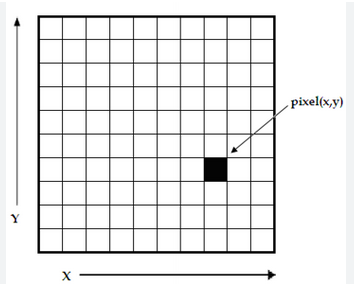
\includegraphics[width=0.55\textwidth]{images/m1_pixel_grid.png}
    \caption{Digital image as a 2D pixel grid: each cell is one pixel located at spatial coordinate $(x, y)$; the shaded cell illustrates a single pixel at position $(x, y)$ with its corresponding intensity value $f(x,y)$. (Source: CV Module 1, Slide 8)}
    \label{fig:m1_pixel_grid}
\end{figure}

The value $f(x, y)$ tells how bright or dark that pixel is:
\begin{itemize}
    \item For a grayscale image: $f(x, y) = 0$ represents black, $f(x, y) = 255$ represents white, and values in between represent shades of gray.
\end{itemize}

\textbf{Example}: $f(100, 50) = 200$ means the pixel at column 100, row 50 has intensity 200 (light gray).

\textbf{Example (RGB)}: $f(100, 50) = (255, 0, 0)$ means the pixel at column 100, row 50 is pure red.

\subsubsection{Continuous vs. Digital Image}

A continuous (analog) image contains infinitely many intensity values across space. When a camera samples it onto a finite grid and quantizes the intensities, the result is a digital image made of discrete pixels. The two images below show the same photograph --- first as a continuous image with a sampling grid overlaid, and then as the resulting pixelated digital version.

\begin{figure}[H]
    \centering
    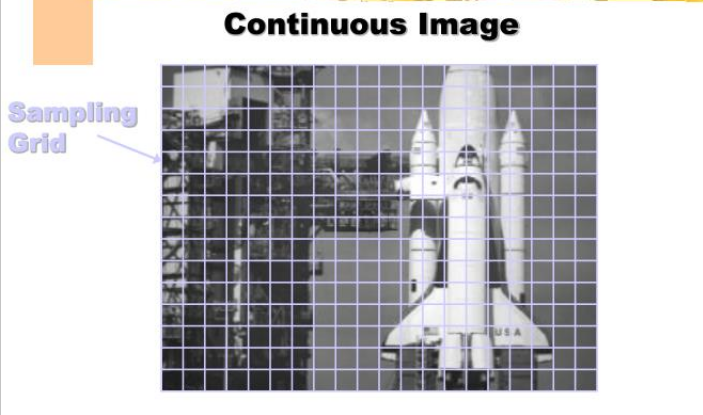
\includegraphics[width=0.85\textwidth]{images/m1_sampling_continuous.png}
    \caption{Continuous image with a sampling grid: the grid defines where the discrete pixel values will be placed during digitization. The finer the grid, the higher the spatial resolution. (Source: CV Module 1, Slide 21)}
    \label{fig:m1_sampling}
\end{figure}

\begin{figure}[H]
    \centering
    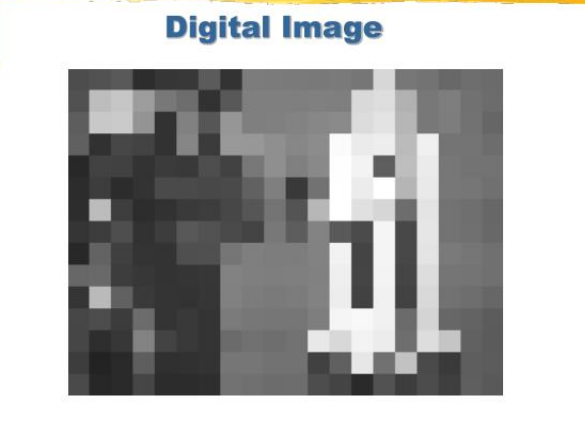
\includegraphics[width=0.65\textwidth]{images/m1_digital_image_pixelated.png}
    \caption{Resulting digital image after sampling: each pixel holds a single intensity value. The blocking artefacts are visible when resolution is low. (Source: CV Module 1, Slide 21)}
    \label{fig:m1_digital_pixelated}
\end{figure}

\subsubsection{Types of Images}

\begin{enumerate}
    \item \textbf{Black and White (Binary) Image}: Contains only two possible pixel values --- black and white. There are no gray levels.
    \item \textbf{8-Bit Grayscale Image}: Has 256 intensity levels ranging from 0 to 255. 0 represents black, 255 represents white, and values in between represent shades of gray (e.g., 127 represents medium gray).
    \item \textbf{16-Bit Image}: Has 65,536 intensity levels (0 to 65,535). Provides much finer intensity detail than an 8-bit image and is commonly used in medical and scientific imaging.
\end{enumerate}

\subsubsection{Pixel, Resolution, and Bit Depth}

\begin{itemize}
    \item \textbf{Pixel}: The smallest unit of an image.
    \item \textbf{Resolution}: Total number of pixels (e.g., $512 \times 512$ = 262,144 pixels).
    \item \textbf{Bit Depth}: Bits per pixel (8-bit = 256 levels).
\end{itemize}

\textbf{Memory Calculation}: For an image of size $256 \times 256$ with bit depth 8:
\[
\text{Memory} = 256 \times 256 \times 8 = 524{,}288 \text{ bits} = 64 \text{ KB}
\]

Higher resolution does not always mean better vision --- processing time and memory increase. Medical images often use 16-bit to capture very small intensity variations important in diagnosis.

\textbf{Dots Per Inch (DPI)}: A measure of spatial resolution indicating how many dots or pixels are present in one inch of an image. Higher DPI means more detail and better image quality, especially in printing and scanning. DPI describes how many pixels or dots are packed into one inch of physical space, while pixel resolution describes the total number of pixels in an image (width $\times$ height).

\begin{tcolorbox}[colback=yellow!5!white,colframe=yellow!75!black,title=\textbf{Worked Example 1: Image Memory Calculation}]
\textbf{Given}: Image size = $1024 \times 768$, Bit depth = 24 bits (RGB)

\textbf{Calculate}: Total memory required in MB.

\textbf{Solution}:
\begin{enumerate}
    \item Total pixels = $1024 \times 768 = 786{,}432$ pixels
    \item Total bits = $786{,}432 \times 24 = 18{,}874{,}368$ bits
    \item Total bytes = $18{,}874{,}368 / 8 = 2{,}359{,}296$ bytes
    \item Total KB = $2{,}359{,}296 / 1024 = 2{,}304$ KB
    \item Total MB = $2{,}304 / 1024 \approx 2.25$ MB
\end{enumerate}

\textbf{Answer}: Approximately \textbf{2.25 MB}.
\end{tcolorbox}

\subsection{Image Acquisition}

\textbf{Image acquisition} is the process of capturing real-world scenes and converting them into digital images. It is the first step in image processing, where a physical scene is sensed and transformed into a digital form.

\textbf{Why Image Acquisition is Important}: All image processing and computer vision tasks depend on image quality. Poor acquisition cannot be fully corrected later. Noise, blur, or low resolution often originate at this stage --- ``Garbage in = Garbage out.''

\subsubsection{Image Acquisition System Components}

An image acquisition system includes:
\begin{enumerate}
    \item \textbf{Imaging Sensor}: Captures energy (light, X-ray, infrared, etc.) and converts it into an analog electrical signal.
    \item \textbf{Sampling}: Converts the continuous spatial signal into discrete pixels.
    \item \textbf{Quantization}: Converts continuous intensity values into discrete digital values.
\end{enumerate}

The pipeline: Camera sensor captures light (analog signal) $\to$ Sampling decides where pixels are placed $\to$ Quantization decides pixel intensity values $\to$ All together form the image acquisition system.

\subsubsection{Three Ways of Image Acquisition}

\begin{enumerate}
    \item \textbf{Single Sensor}: Uses one imaging sensor. Example: Old fax machine --- scans the scene point by point to form an image.
    \item \textbf{Sensor Array}: Uses multiple sensors arranged in 1D or 2D. Example: Digital camera or mobile phone camera --- captures the entire image at once.
    \item \textbf{Line Scan Sensor}: Uses a 1D array of sensors. Example: Barcode scanner --- uses a 1D sensor array and forms the image line by line using motion.
\end{enumerate}

\subsubsection{Complete Acquisition Pipeline}

\begin{enumerate}
    \item \textbf{Illumination (Energy) Source}: Provides energy (light, X-ray, infrared, etc.) to illuminate the scene.
    \item \textbf{Scene Element}: The object or physical scene that reflects or emits energy.
    \item \textbf{Imaging System}: Captures the reflected energy and forms an image on the image plane using lenses and sensors.
    \item \textbf{Internal Image Plane}: Continuous (analog) image formed before digitization.
    \item \textbf{Digitization}: Sampling and quantization convert the analog image into digital form.
    \item \textbf{Output (Digitized Image)}: Final digital image represented as a grid of pixels.
\end{enumerate}

\begin{center}
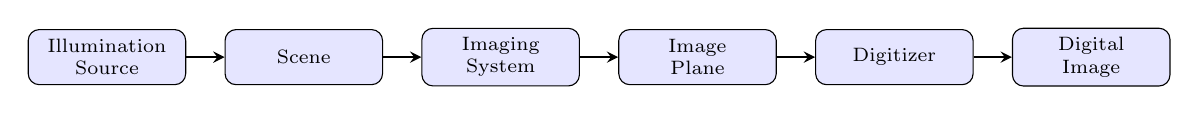
\begin{tikzpicture}[
    node distance=1.2cm,
    box/.style={rectangle, draw, rounded corners, minimum width=2cm, minimum height=0.7cm, font=\scriptsize, align=center, fill=blue!10},
    arrow/.style={->, >=stealth, thick}
]
\node[box] (illum) at (0,0) {Illumination\\Source};
\node[box] (scene) at (2.5,0) {Scene};
\node[box] (imaging) at (5,0) {Imaging\\System};
\node[box] (plane) at (7.5,0) {Image\\Plane};
\node[box] (digit) at (10,0) {Digitizer};
\node[box] (output) at (12.5,0) {Digital\\Image};

\draw[arrow] (illum) -- (scene);
\draw[arrow] (scene) -- (imaging);
\draw[arrow] (imaging) -- (plane);
\draw[arrow] (plane) -- (digit);
\draw[arrow] (digit) -- (output);

\end{tikzpicture}
\end{center}
\captionof{figure}{Image Acquisition Pipeline: From illumination source to digital image output.}

\begin{tcolorbox}[colback=yellow!5!white,colframe=yellow!75!black,title=\textbf{Worked Example 2: Sampling and Quantization}]
\textbf{Given}: A continuous image with intensity range $[0, 10]$ volts is to be digitized with 4-bit quantization.

\textbf{Calculate}: Number of intensity levels and the step size.

\textbf{Solution}:
\begin{enumerate}
    \item Number of intensity levels = $2^4 = 16$ levels (0 to 15).
    \item Step size = $(10 - 0) / 16 = 0.625$ volts per level.
    \item A continuous value of 3.2 volts would be quantized to level $\lfloor 3.2 / 0.625 \rfloor = \lfloor 5.12 \rfloor = 5$.
    \item Reconstructed value = $5 \times 0.625 = 3.125$ volts.
    \item Quantization error = $3.2 - 3.125 = 0.075$ volts.
\end{enumerate}
\end{tcolorbox}

\subsection{Image Preprocessing}

\textbf{Image preprocessing} consists of operations applied to an acquired image to improve its quality and remove imperfections before further analysis. Preprocessing mainly includes low-level operations such as:
\begin{itemize}
    \item Noise reduction
    \item Smoothing and filtering
    \item Contrast enhancement
    \item Histogram equalization
    \item Image sharpening
    \item Image resizing and normalization
    \item Image restoration (basic level)
\end{itemize}

Raw images cannot be directly used for face recognition because they contain noise, lighting variations, and background clutter. Preprocessing is required.

\begin{figure}[H]
    \centering
    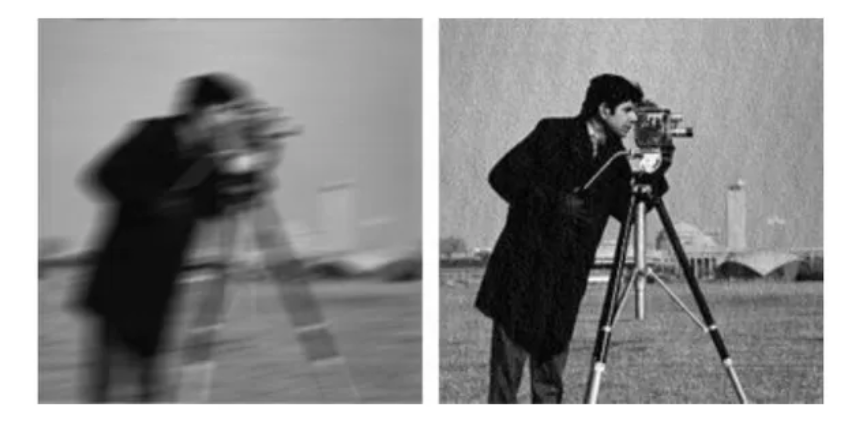
\includegraphics[width=0.85\textwidth]{images/m1_blur_vs_sharp.png}
    \caption{Preprocessing effect on image quality: left --- blurred image with low spatial detail; right --- sharp image after contrast-preserving restoration. This demonstrates why preprocessing is essential before analysis. (Source: CV Module 1, Slide 24)}
    \label{fig:m1_blur_vs_sharp}
\end{figure}

\begin{figure}[H]
    \centering
    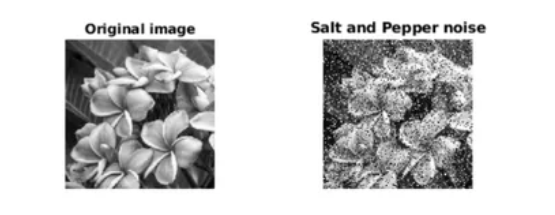
\includegraphics[width=0.85\textwidth]{images/m1_salt_pepper_noise.png}
    \caption{Salt-and-pepper noise: original image (left) vs. image corrupted by random black and white pixel noise (right). Median filtering is the standard preprocessing technique to remove this type of noise. (Source: CV Module 1, Slide 26)}
    \label{fig:m1_salt_pepper}
\end{figure}

\subsubsection{Image Segmentation and Representation (Pipeline Overview)}

Before discussing transforms, the full preprocessing-to-analysis pipeline is: image acquisition $\to$ preprocessing $\to$ segmentation $\to$ representation $\to$ vision task. Segmentation divides the image into meaningful regions; representation stores those regions compactly for downstream tasks.

\begin{figure}[H]
    \centering
    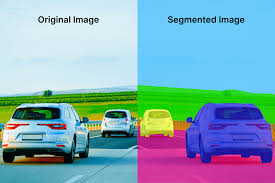
\includegraphics[width=0.85\textwidth]{images/m1_segmentation_example.png}
    \caption{Image segmentation example: the original traffic scene (left) is divided into colour-coded regions --- each car is assigned a distinct colour label in the segmented output (right). (Source: CV Module 1, Slide 28)}
    \label{fig:m1_segmentation_example}
\end{figure}

\begin{figure}[H]
    \centering
    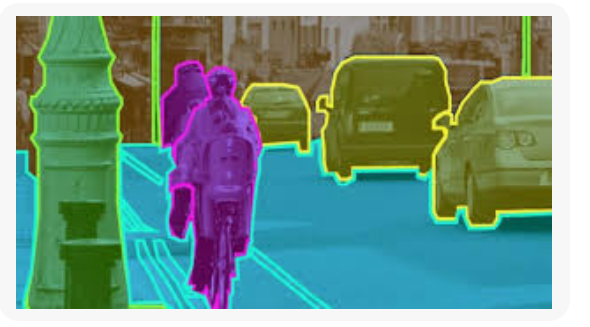
\includegraphics[width=0.85\textwidth]{images/m1_semantic_segmentation.png}
    \caption{Semantic segmentation of a street scene: every pixel is labelled by class (person, cyclist, car, road, building). Unlike bounding-box detection, segmentation provides pixel-level understanding. (Source: CV Module 1, Slide 29)}
    \label{fig:m1_semantic_segmentation}
\end{figure}

\subsubsection{Image Transforms}

\textbf{Image transforms} are mathematical techniques that convert an image from the spatial domain (pixel values) into another domain, usually the frequency domain, to make image analysis, enhancement, filtering, and compression easier.

\textbf{Types of Image Transforms}:
\begin{enumerate}
    \item \textbf{Fourier Transform}: Converts an image from spatial domain to frequency domain. Separates the image into low-frequency components (smooth regions) and high-frequency components (edges and details). Used for noise removal, filtering, and image enhancement. (Reference: Gonzalez \& Woods, Chapter 4)
    \item \textbf{Discrete Cosine Transform (DCT)}: Represents an image using only cosine functions. Concentrates most image information into a few low-frequency coefficients. Used mainly for image compression (e.g., JPEG).
    \item \textbf{Wavelet Transform}: Represents an image at multiple resolutions by analyzing both spatial and frequency information. Useful for capturing local image details and edges. Used for image denoising, compression, and feature extraction.
\end{enumerate}

\begin{tcolorbox}[colback=yellow!5!white,colframe=yellow!75!black,title=\textbf{Worked Example 3: DCT Coefficient Energy Compaction}]
\textbf{Given}: A $2 \times 2$ image block with pixel values:
\[
I = \begin{bmatrix} 10 & 10 \\ 10 & 10 \end{bmatrix}
\]

\textbf{Calculate}: The 2D-DCT coefficients.

\textbf{Solution}:
For a uniform block, all pixels have the same value (10). The DC coefficient (average) is:
\[
F(0,0) = \frac{1}{2}(10 + 10 + 10 + 10) = 20
\]
All AC coefficients (high-frequency) are \textbf{zero} because there is no variation.

\textbf{Interpretation}: DCT concentrates all energy in the DC coefficient, demonstrating why DCT is excellent for compression --- smooth regions need very few coefficients.
\end{tcolorbox}

\subsection{Morphological Image Processing}

\textbf{Morphological image processing} is a collection of non-linear operations that process images based on their shape and structure. These operations use a \textbf{structuring element} (like a kernel or mask) to probe and modify objects in a binary image (and sometimes grayscale images). Main purpose: to clean shapes, remove noise, fill gaps, separate or connect objects before analysis.

\subsubsection{Basic Morphological Operations}

\begin{enumerate}
    \item \textbf{Erosion}: Shrinks objects by removing boundary pixels.
    \begin{itemize}
        \item The structuring element slides over the image.
        \item A pixel remains white (1) only if all pixels under the structuring element are white.
        \item If any pixel under the structuring element is black, the center pixel becomes black.
        \item \textbf{Rule}: If ALL pixels under the kernel are 1, center pixel stays 1. If ANY pixel is 0, center pixel becomes 0.
        \item \textbf{Effects}: Objects become thinner; small noise is removed; narrow connections may break.
        \item \textbf{Use cases}: Remove small white noise; separate touching objects.
    \end{itemize}

    \item \textbf{Dilation}: Expands objects by adding pixels to their boundaries.
    \begin{itemize}
        \item The structuring element slides over the image.
        \item If any pixel under the structuring element is white, the center pixel becomes white.
        \item \textbf{Effects}: Objects become thicker; small holes are filled; close objects may merge.
        \item \textbf{Use cases}: Fill small gaps; connect broken parts of objects.
    \end{itemize}

    \item \textbf{Opening}: Erosion followed by Dilation.
    \begin{itemize}
        \item First erosion removes small noise; then dilation restores the main object size.
        \item \textbf{Effects}: Removes small objects; smooths object boundaries; preserves shape of larger objects.
        \item \textbf{Use cases}: Remove salt noise; remove thin protrusions.
    \end{itemize}

    \item \textbf{Closing}: Dilation followed by Erosion.
    \begin{itemize}
        \item First dilation fills gaps and holes; then erosion restores object shape.
        \item \textbf{Effects}: Fills small holes; closes narrow breaks; smooths boundaries.
        \item \textbf{Use cases}: Fill gaps in characters or objects; repair broken contours.
    \end{itemize}

    \item \textbf{Hit-or-Miss Transformation}: Detects specific shapes or patterns.
    \begin{itemize}
        \item Uses two structuring elements: one matches foreground (object), one matches background.
        \item A pixel is marked only if both conditions match exactly.
        \item \textbf{Use cases}: Shape detection; symbol or pattern recognition.
    \end{itemize}
\end{enumerate}

\begin{center}
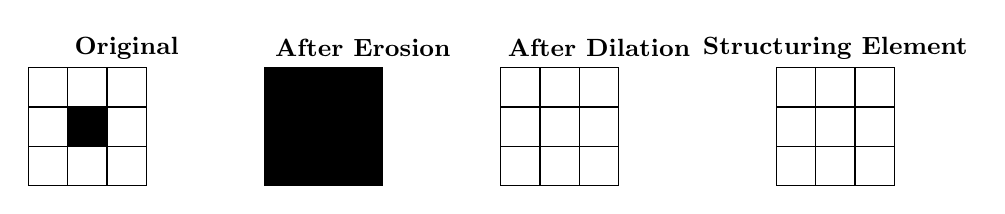
\begin{tikzpicture}[
    node distance=0.3cm,
    pixel/.style={rectangle, draw, minimum size=0.5cm, font=\tiny},
    whitepix/.style={pixel, fill=white},
    blackpix/.style={pixel, fill=black},
    label/.style={font=\small, align=center}
]
% Original Object
\node[label] at (1, 2.5) {\textbf{Original}};
\node[whitepix] at (0, 2) {};
\node[whitepix] at (0.5, 2) {};
\node[whitepix] at (1, 2) {};
\node[whitepix] at (0, 1.5) {};
\node[blackpix] at (0.5, 1.5) {};
\node[whitepix] at (1, 1.5) {};
\node[whitepix] at (0, 1) {};
\node[whitepix] at (0.5, 1) {};
\node[whitepix] at (1, 1) {};

% Erosion
\node[label] at (4, 2.5) {\textbf{After Erosion}};
\node[blackpix] at (3, 2) {};
\node[blackpix] at (3.5, 2) {};
\node[blackpix] at (4, 2) {};
\node[blackpix] at (3, 1.5) {};
\node[blackpix] at (3.5, 1.5) {};
\node[blackpix] at (4, 1.5) {};
\node[blackpix] at (3, 1) {};
\node[blackpix] at (3.5, 1) {};
\node[blackpix] at (4, 1) {};

% Dilation
\node[label] at (7, 2.5) {\textbf{After Dilation}};
\node[whitepix] at (6, 2) {};
\node[whitepix] at (6.5, 2) {};
\node[whitepix] at (7, 2) {};
\node[whitepix] at (6, 1.5) {};
\node[whitepix] at (6.5, 1.5) {};
\node[whitepix] at (7, 1.5) {};
\node[whitepix] at (6, 1) {};
\node[whitepix] at (6.5, 1) {};
\node[whitepix] at (7, 1) {};

% SE
\node[label] at (10, 2.5) {\textbf{Structuring Element}};
\node[whitepix] at (9.5, 2) {};
\node[whitepix] at (10, 2) {};
\node[whitepix] at (10.5, 2) {};
\node[whitepix] at (9.5, 1.5) {};
\node[whitepix] at (10, 1.5) {};
\node[whitepix] at (10.5, 1.5) {};
\node[whitepix] at (9.5, 1) {};
\node[whitepix] at (10, 1) {};
\node[whitepix] at (10.5, 1) {};

\end{tikzpicture}
\end{center}
\captionof{figure}{Morphological operations concept: Original binary object, after erosion (shrinks), after dilation (expands), and the structuring element (3$\times$3 kernel).}

\subsubsection{Morphological Algorithms}

\begin{itemize}
    \item \textbf{Boundary Extraction}: Extracts only the boundary (outline) of an object. Obtained by subtracting the eroded image from the original image. Helps in shape analysis and object localization.
    \item \textbf{Region Filling}: Fills holes or enclosed regions inside an object. Starts from a seed point inside the region and expands until the boundary is reached. Used to remove holes in binary objects.
    \item \textbf{Connected Components}: Identifies and labels separate objects in a binary image. Pixels are grouped based on connectivity (4-connected or 8-connected). Used for object counting and region-based analysis.
    \item \textbf{Thinning}: Reduces objects to one-pixel-wide lines. Preserves the overall structure and connectivity. Used in handwriting and fingerprint analysis.
    \item \textbf{Skeletonization}: Produces the medial axis (skeleton) of an object. Represents shape using minimum pixels while preserving topology. Useful for shape recognition and matching.
\end{itemize}

\textbf{Easy Recall}:
\begin{itemize}
    \item Boundary = outline
    \item Region filling = fill holes
    \item Connected components = separate objects
    \item Thinning = make thin
    \item Skeleton = shape backbone
\end{itemize}

\begin{figure}[H]
    \centering
    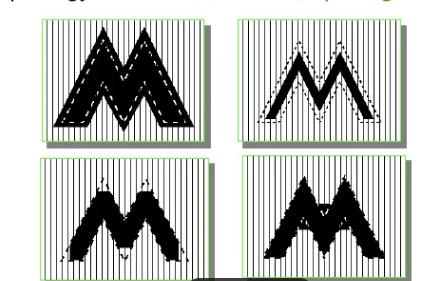
\includegraphics[width=0.85\textwidth]{images/m1_erosion_dilation_letter.png}
    \caption{Erosion effect on the letter ``M'': the four panels show (top-left) original binary object, (top-right) after erosion the object shrinks and thin parts break, (bottom-left) after stronger erosion even more detail is lost, (bottom-right) erosion removes noise while preserving larger structures. (Source: CV Module 1, Slide 39)}
    \label{fig:m1_erosion_letter}
\end{figure}

\begin{figure}[H]
    \centering
    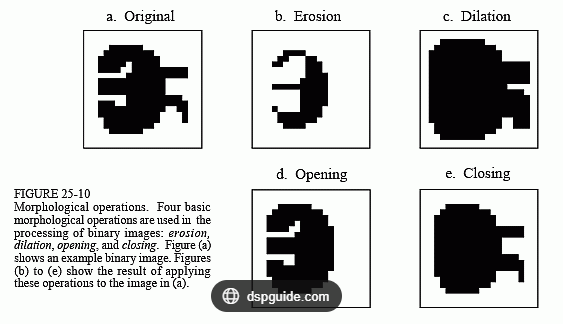
\includegraphics[width=0.85\textwidth]{images/m1_morphological_operations.png}
    \caption{All four basic morphological operations on digit ``3'': (a) original binary image; (b) erosion --- object shrinks; (c) dilation --- object expands; (d) opening (erosion then dilation) --- removes small noise; (e) closing (dilation then erosion) --- fills small holes. (Source: CV Module 1, Slide 45, dspguide.com)}
    \label{fig:m1_morphological_ops}
\end{figure}

\begin{tcolorbox}[colback=yellow!5!white,colframe=yellow!75!black,title=\textbf{Worked Example 4: Morphological Opening and Closing}]
\textbf{Given}: A binary image contains a large square object with small white noise dots (salt noise) scattered around it, and a small hole inside the square.

\textbf{Task}: Remove the salt noise and fill the hole.

\textbf{Solution}:
\begin{enumerate}
    \item \textbf{Step 1 -- Opening}: Apply erosion followed by dilation with a $3 \times 3$ structuring element.
    \begin{itemize}
        \item Erosion removes the small noise dots (they are smaller than the structuring element).
        \item Dilation restores the original size of the square.
        \item Result: Square is clean, noise is gone, but the hole remains.
    \end{itemize}
    \item \textbf{Step 2 -- Closing}: Apply dilation followed by erosion with a $3 \times 3$ structuring element.
    \begin{itemize}
        \item Dilation fills the hole inside the square.
        \item Erosion restores the square to its original size.
        \item Result: Square is clean with no hole.
    \end{itemize}
\end{enumerate}

\textbf{Final Result}: Opening removes noise; Closing fills holes. Both operations preserve the main object.
\end{tcolorbox}

\subsection{Preprocessing Challenges and Solutions}

\begin{enumerate}
    \item \textbf{Clutter}: Background contains unnecessary objects that confuse the target.
    \begin{itemize}
        \item \textbf{Solutions}: Image segmentation, morphological opening, background subtraction, ROI (Region of Interest) cropping.
        \item \textbf{Example}: Detecting a car when trees, people, and buildings are also present.
    \end{itemize}

    \item \textbf{Deformation}: Same object appears in different shapes or poses.
    \begin{itemize}
        \item \textbf{Solutions}: Morphological operations, edge detection, shape normalization, skeletonization.
        \item \textbf{Example}: Handwritten digit ``2'' written differently by different people.
    \end{itemize}

    \item \textbf{Intra-class Variation}: Objects of the same class look different in size, color, texture, or orientation.
    \begin{itemize}
        \item \textbf{Solutions}: Image resizing and normalization, histogram equalization, color space conversion (RGB $\to$ Gray/HSV).
        \item \textbf{Example}: Faces with different skin tones, lighting, or expressions.
    \end{itemize}

    \item \textbf{Gaussian Noise}: Random intensity fluctuations caused by sensors or low light.
    \begin{itemize}
        \item \textbf{Solutions}: Gaussian blur, median filtering, bilateral filtering.
        \item \textbf{Example}: Grainy medical or satellite images.
    \end{itemize}

    \item \textbf{Illumination Variations}: Changes in image appearance caused by lighting, not by the object itself.
    \begin{itemize}
        \item \textbf{Problems}: Pixel intensity changes even when object is same; edges may disappear or false edges appear; ML models may fail due to lighting bias.
        \item \textbf{Solutions}: Intensity normalization, histogram equalization, adaptive histogram equalization (CLAHE), log/gamma correction, mean-variance normalization.
    \end{itemize}
\end{enumerate}

\newpage

\section{Module 2: Shape Analysis, Edge Detection, and Segmentation}

\subsection{Introduction to Shape Analysis}

Shape analysis is the process of understanding what an object looks like using its outline or its area. Humans do this naturally, but computer vision tries to teach computers the same skill using mathematics.

\textbf{Why Shape Analysis is Hard for Computers}:
\begin{enumerate}
    \item \textbf{Rotation}: For humans, only orientation has changed. For a computer, rotation changes pixel positions completely.
    \item \textbf{Scale}: Near object = more pixels; far object = fewer pixels. Different size = different pixel count.
    \item \textbf{Noise}: Poor imaging conditions (cheap cameras, low light, rain/fog) introduce noise, breaking true edges and creating false boundaries.
    \item \textbf{Occlusion}: When objects are partially hidden, humans mentally complete the shape, but computers need mathematical models to infer missing boundaries.
\end{enumerate}

\begin{figure}[H]
    \centering
    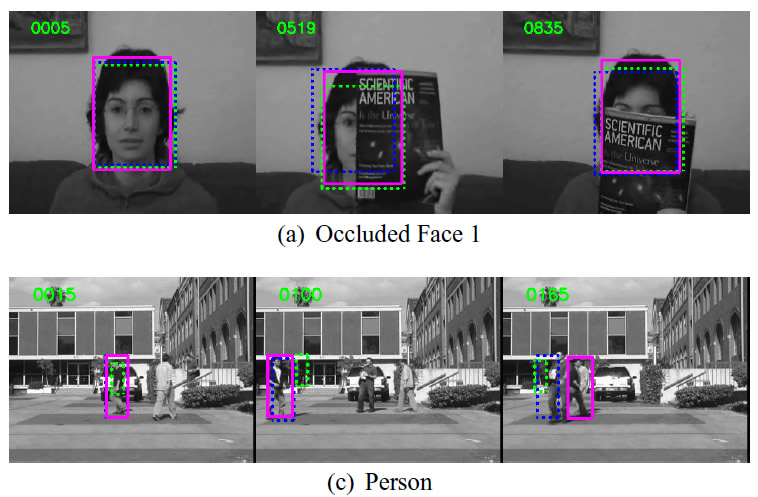
\includegraphics[width=0.85\textwidth]{images/m2_occlusion_examples.png}
    \caption{Shape analysis challenge --- Occlusion: (top) a face is progressively occluded by a book across three frames (0005, 0519, 0835), requiring the tracker to infer the partially hidden face shape; (bottom) a person is occluded by other pedestrians in a crowd scene. These examples show why shape descriptions must be robust to partial visibility. (Source: CV Module 2, Slide 10)}
    \label{fig:m2_occlusion}
\end{figure}

\begin{figure}[H]
    \centering
    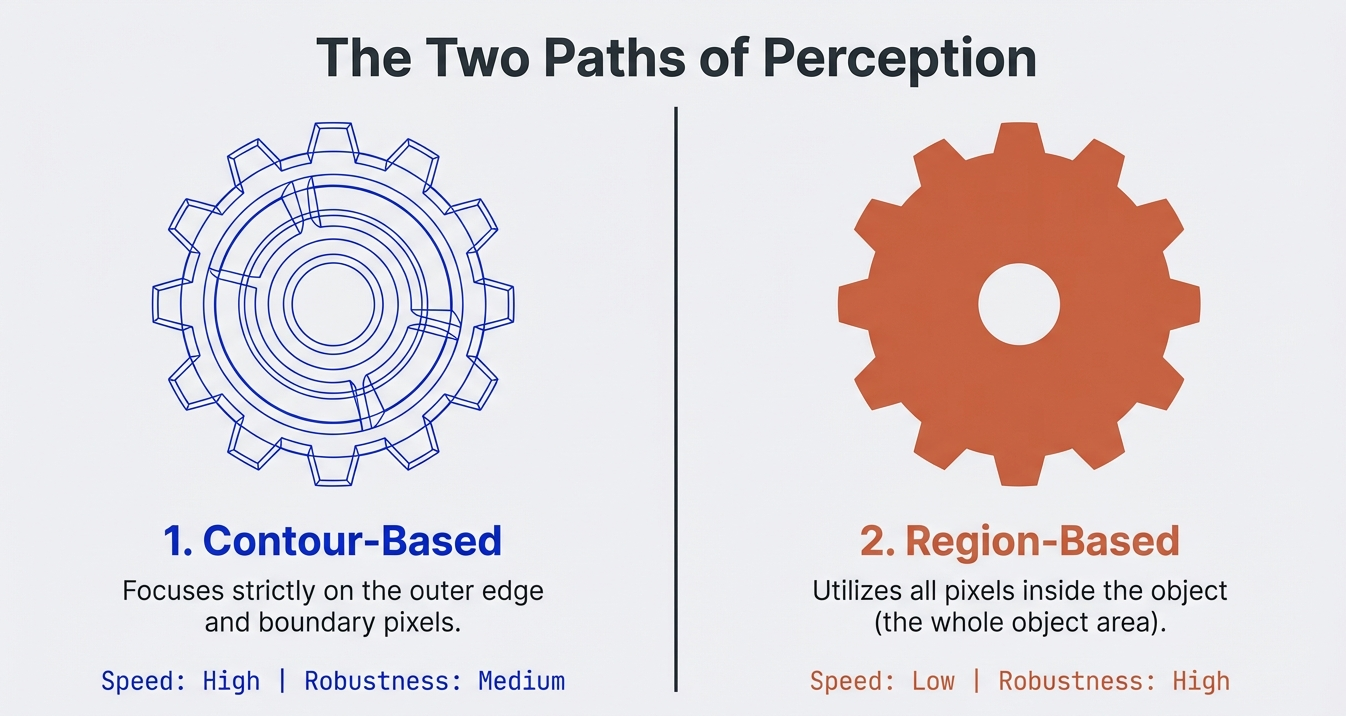
\includegraphics[width=0.85\textwidth]{images/m2_contour_vs_region.png}
    \caption{Two approaches to shape description: Contour-Based methods (left gear, blue) focus strictly on boundary pixels --- fast but moderately robust; Region-Based methods (right gear, orange) use all pixels inside the object --- slower but highly robust to noise and occlusion. (Source: CV Module 2, Slide 41)}
    \label{fig:m2_contour_vs_region}
\end{figure}

We need shape descriptions that are robust to rotation, scale, and noise. Two main approaches exist:
\begin{itemize}
    \item \textbf{Contour-based (Boundary) Methods}: Chain codes, boundary representation, Fourier descriptors.
    \item \textbf{Region-based Methods}: Area, perimeter, moments, convex hull, skeletons.
\end{itemize}

\begin{figure}[H]
    \centering
    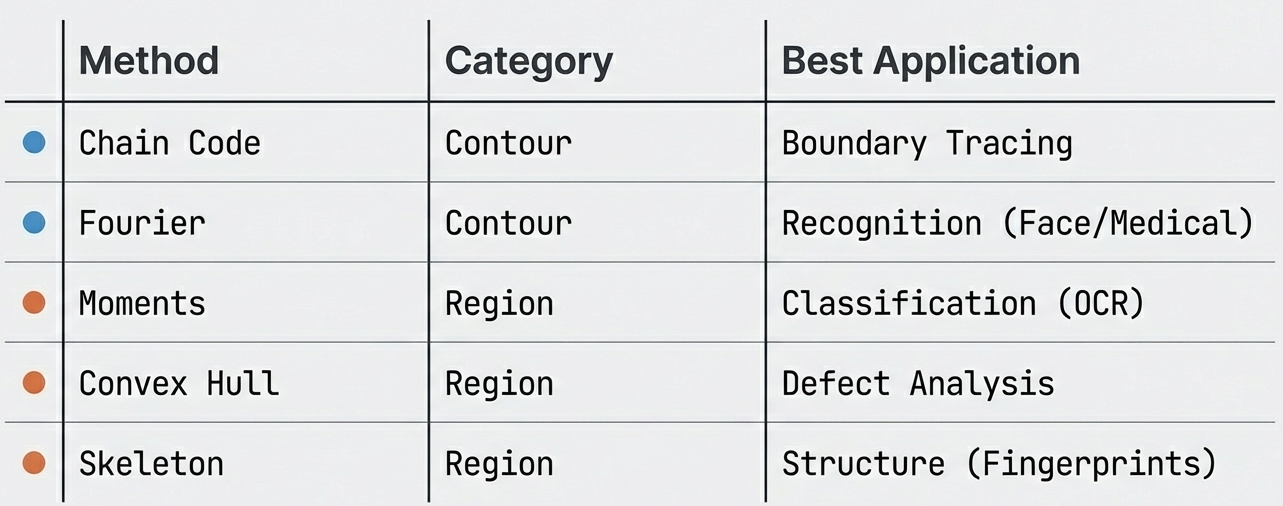
\includegraphics[width=0.85\textwidth]{images/m2_shape_methods_comparison.png}
    \caption{Comparison of shape representation methods: Chain Code and Fourier are contour-based (use only boundary pixels), suited to boundary tracing and recognition; Moments, Convex Hull, and Skeleton are region-based, using all interior pixels, suited to classification, defect analysis, and structural matching. (Source: CV Module 2, Slide 55)}
    \label{fig:m2_methods_comparison}
\end{figure}

\begin{figure}[H]
    \centering
    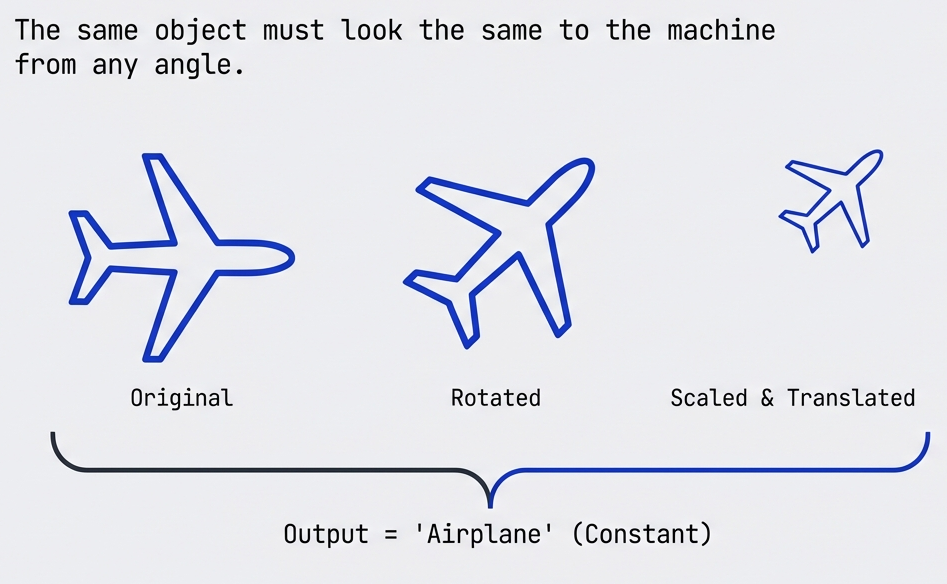
\includegraphics[width=0.85\textwidth]{images/m2_shape_invariants.png}
    \caption{Shape invariance requirement: the same airplane object shown in its original pose, rotated, and scaled-and-translated must all produce the same shape descriptor output ``Airplane''. Good shape descriptors are invariant to rotation, scale, and translation. (Source: CV Module 2, Slide 40)}
    \label{fig:m2_shape_invariants}
\end{figure}

\subsection{Contour-Based Shape Representation}

A \textbf{boundary} is the set of pixels that separate the object from the background. A \textbf{contour} is the ordered tracing of that boundary, usually represented as a curve. Contours represent the outline (shape) of an object and separate it from the background.

\begin{figure}[H]
    \centering
    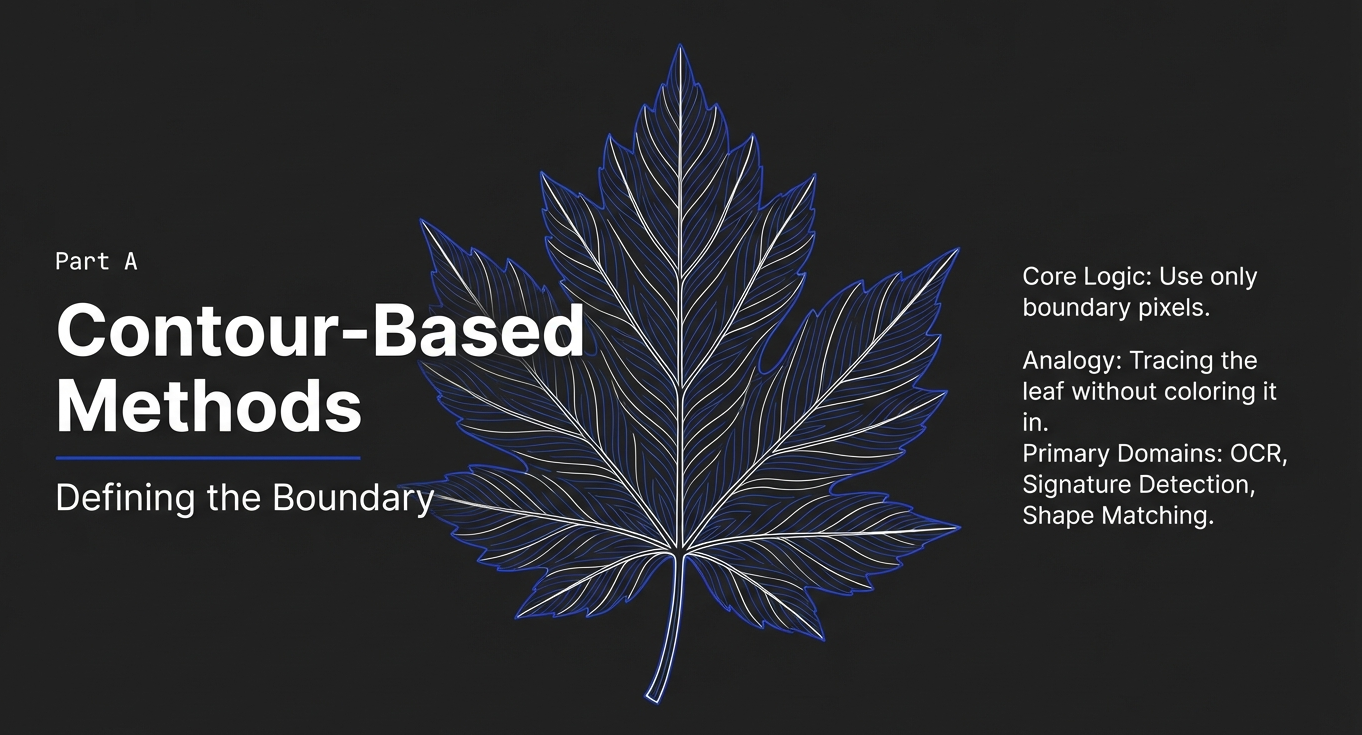
\includegraphics[width=0.85\textwidth]{images/m2_contour_based_intro.png}
    \caption{Contour-Based Methods --- defining the boundary: the leaf outline (blue border) illustrates the core logic of tracing only the boundary pixels without filling the interior. Primary domains: OCR, signature detection, shape matching. (Source: CV Module 2, Slide 42)}
    \label{fig:m2_contour_intro}
\end{figure}

\begin{figure}[H]
    \centering
    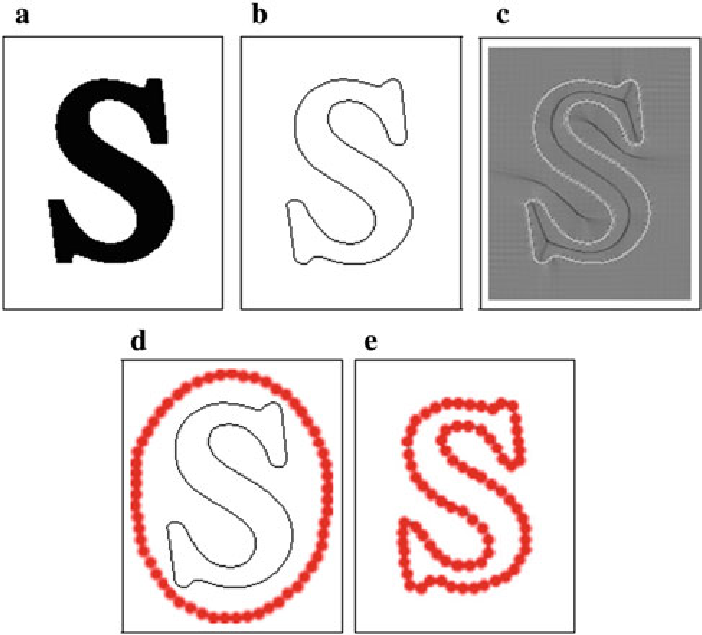
\includegraphics[width=0.85\textwidth]{images/m2_contour_representation_S.png}
    \caption{Contour representation of the letter ``S'': (a) original binary image; (b) simple contour trace --- inner and outer boundary; (c) morphological gradient highlighting the boundary region; (d) external boundary points (red dots around the convex outline); (e) exact boundary points (red dots following the actual letter outline). (Source: CV Module 2, Slide 12)}
    \label{fig:m2_contour_S}
\end{figure}

\subsubsection{Chain Codes (Freeman Chain Codes)}

Imagine walking along the boundary of an object on graph paper. Instead of storing all pixel coordinates, you just record which direction you move next. That direction sequence = \textbf{Chain Code}.

\textbf{4-Direction Chain Code}:
\begin{itemize}
    \item Move right = 0, Move up = 2, Move left = 4, Move down = 6
    \item Boundary becomes: 0, 0, 2, 2, 4, 4, 6, 6, ...
\end{itemize}

\textbf{8-Direction Chain Code}: Uses 8 directions (including diagonals):

\begin{figure}[H]
    \centering
    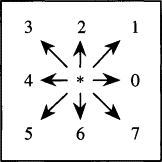
\includegraphics[width=0.45\textwidth]{images/m2_chaincode_directions_8way.png}
    \caption{8-directional Freeman chain code compass: directions 0--7 emanating from the current pixel (centre asterisk). Direction 0 = right, 1 = upper-right, 2 = up, 3 = upper-left, 4 = left, 5 = lower-left, 6 = down, 7 = lower-right. (Source: CV Module 2, Slide 16)}
    \label{fig:m2_chaincode_compass}
\end{figure}

\begin{figure}[H]
    \centering
    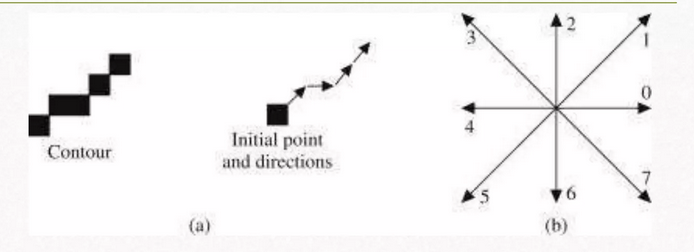
\includegraphics[width=0.85\textwidth]{images/m2_chaincode_contour_compass.png}
    \caption{Chain code setup: (a) a diagonal contour traced from its initial point with direction arrows; (b) the 8-direction compass numbered 0--7. The chain code for this contour encodes which direction arrow is followed at each boundary pixel step. (Source: CV Module 2, Slide 16)}
    \label{fig:m2_chaincode_contour}
\end{figure}

\begin{figure}[H]
    \centering
    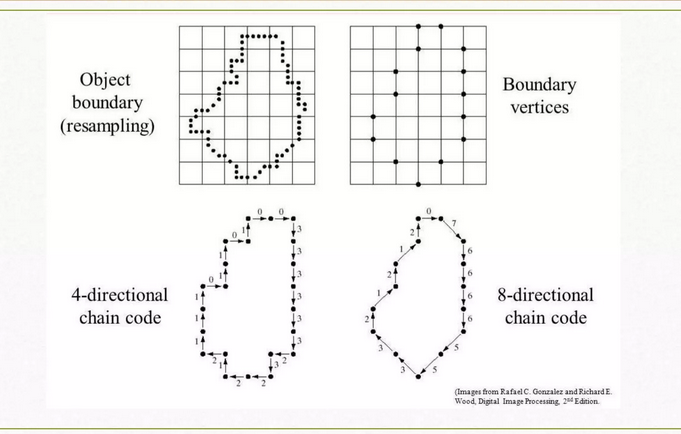
\includegraphics[width=0.85\textwidth]{images/m2_chaincode_4dir_8dir.png}
    \caption{4-directional and 8-directional chain codes (Gonzalez \& Woods): the object boundary (top-left) is resampled onto a coarser grid (top-right, ``boundary vertices''); the 4-directional chain code (bottom-left) traces the object using only horizontal/vertical steps, while the 8-directional code (bottom-right) also includes diagonals for a more compact representation. (Source: CV Module 2, Slide 24)}
    \label{fig:m2_chaincode_4dir8dir}
\end{figure}

\begin{figure}[H]
    \centering
    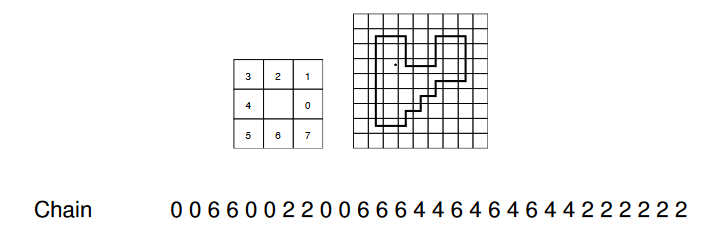
\includegraphics[width=0.85\textwidth]{images/m2_chaincode_worked_example.png}
    \caption{Worked chain code example: the object boundary (irregular staircase shape on the grid, right) is traced from the starting cell. The 8-directional compass (left) defines direction numbers; the resulting chain code is ``0066002200666444646464422222''. (Source: CV Module 2, Slide 23)}
    \label{fig:m2_chaincode_worked}
\end{figure}

\begin{figure}[H]
    \centering
    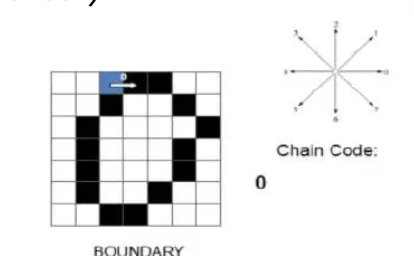
\includegraphics[width=0.85\textwidth]{images/m2_chaincode_tracing_step.png}
    \caption{Step-by-step chain code tracing: starting at pixel $p$ (blue), the first move is direction 0 (right), and the chain code begins ``0''. The grid and 8-direction compass show how each successive boundary pixel contributes one code digit. (Source: CV Module 2, Slide 26)}
    \label{fig:m2_chaincode_step}
\end{figure}

\begin{figure}[H]
    \centering
    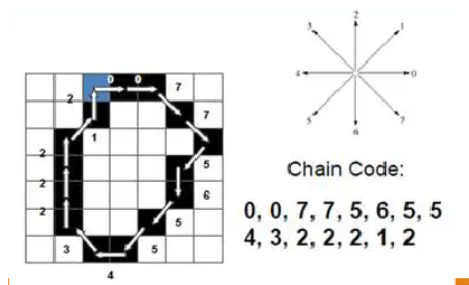
\includegraphics[width=0.85\textwidth]{images/m2_chaincode_ring_example.png}
    \caption{Complete chain code example on a ring-shaped contour: the traced boundary with direction arrows yields chain code ``0, 0, 7, 7, 5, 6, 5, 5, 4, 3, 2, 2, 2, 1, 2''. The 8-direction compass is shown top-right. (Source: CV Module 2, Slide 27)}
    \label{fig:m2_chaincode_ring}
\end{figure}

\textbf{Chain Code Invariance Properties}:

\begin{figure}[H]
    \centering
    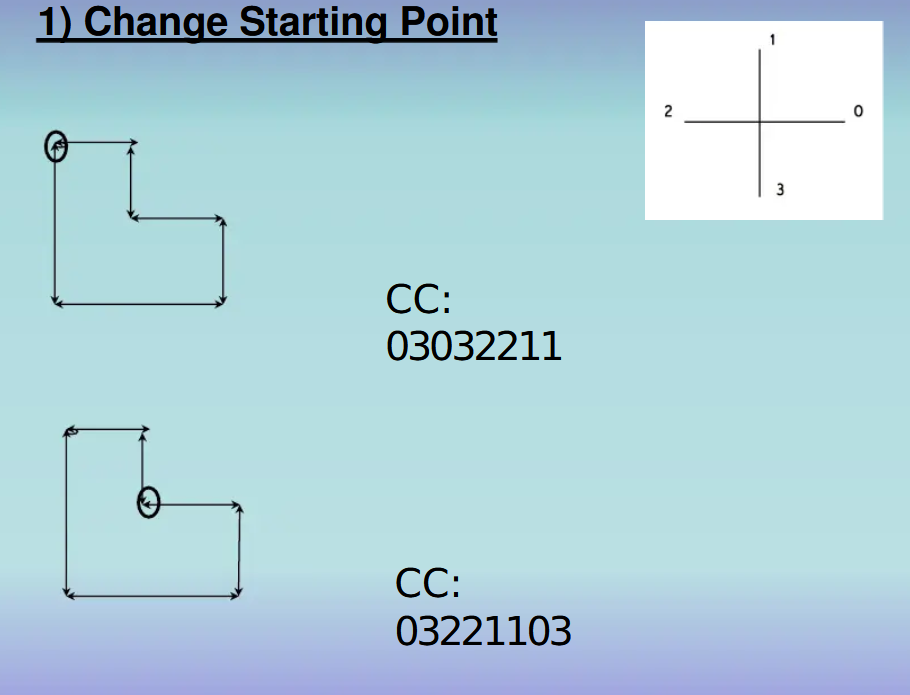
\includegraphics[width=0.85\textwidth]{images/m2_chaincode_start_point.png}
    \caption{Chain code --- change of starting point: the same L-shaped contour traced from two different starting pixels produces different chain codes (CC: 03032211 vs 03221103). The shape is identical but the code sequence differs, hence normalization is needed for start-point invariance. (Source: CV Module 2, Slide 18)}
    \label{fig:m2_cc_start}
\end{figure}

\begin{figure}[H]
    \centering
    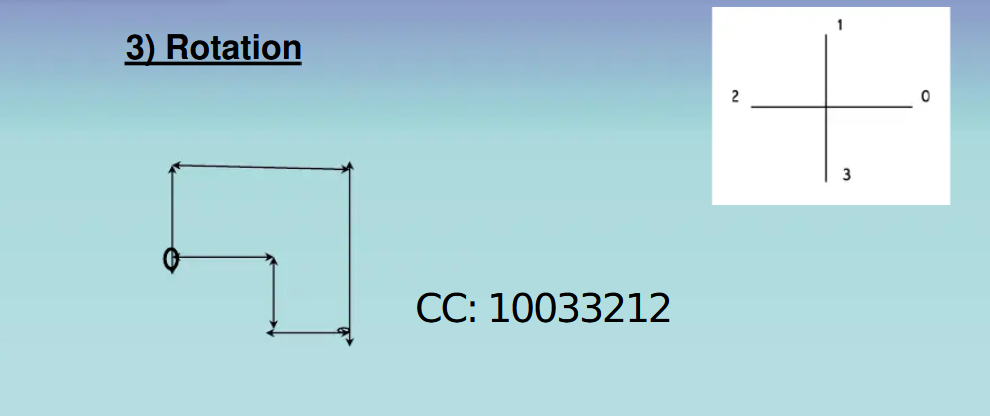
\includegraphics[width=0.75\textwidth]{images/m2_chaincode_rotation.png}
    \caption{Chain code --- rotation sensitivity: the same L-shape rotated 90° produces a completely different chain code (CC: 10033212 vs original), demonstrating that simple chain codes are NOT rotation invariant. The Circular First Difference normalizes this. (Source: CV Module 2, Slide 20)}
    \label{fig:m2_cc_rotation}
\end{figure}

\textbf{Limitations of Chain Codes}:
\begin{itemize}
    \item \textbf{Sensitive to rotation}: Rotating the object changes the direction numbers completely.
    \item \textbf{Sensitive to noise}: Small boundary irregularities create large changes in the code.
    \item \textbf{Depends on starting point}: Different starting pixels give different chain code sequences.
    \item \textbf{Not scale invariant}: Larger or smaller objects produce longer or shorter codes.
\end{itemize}

\textbf{Solutions}: Normalization using Circular First Difference (CFD) and normalized CFD.

\begin{tcolorbox}[colback=yellow!5!white,colframe=yellow!75!black,title=\textbf{Worked Example 5: Chain Code Extraction}]
\textbf{Given}: A simple square object traced clockwise from top-left corner.

\textbf{Trace}: Right $\to$ Right $\to$ Down $\to$ Down $\to$ Left $\to$ Left $\to$ Up $\to$ Up

\textbf{8-Direction Chain Code}: 0, 0, 6, 6, 4, 4, 2, 2

\textbf{Normalization}: Compute differences between consecutive directions (circular):
\begin{itemize}
    \item Differences: $(0-0)=0$, $(0-6)=-6 \equiv 2$ (mod 8), $(6-6)=0$, $(6-4)=2$, $(4-4)=0$, $(4-2)=2$, $(2-2)=0$, $(2-0)=2$
    \item Normalized Chain Code (CFD): 0, 2, 0, 2, 0, 2, 0, 2
\end{itemize}

\textbf{Property}: The normalized code is \textbf{rotation invariant} --- rotating the square gives the same CFD regardless of starting direction.
\end{tcolorbox}

\subsubsection{Fourier Descriptors}

Instead of describing shape in the spatial domain, Fourier descriptors describe it in the frequency domain.

\textbf{Process}:
\begin{enumerate}
    \item Convert the boundary into a complex signal (x + iy coordinates).
    \item Apply the Discrete Fourier Transform (DFT).
    \item Keep the first $P$ coefficients (low frequencies = overall shape; high frequencies = fine details).
\end{enumerate}

\textbf{Properties}:
\begin{itemize}
    \item Low frequencies = overall shape; high frequencies = fine details.
    \item Small $P$ = coarse shape; large $P$ = detailed shape.
    \item Can be made invariant to translation, rotation, and scale after normalization.
\end{itemize}

\textbf{Limitations}: Needs closed boundary; loses exact pixel-level detail; not ideal for very irregular shapes.

\begin{figure}[H]
    \centering
    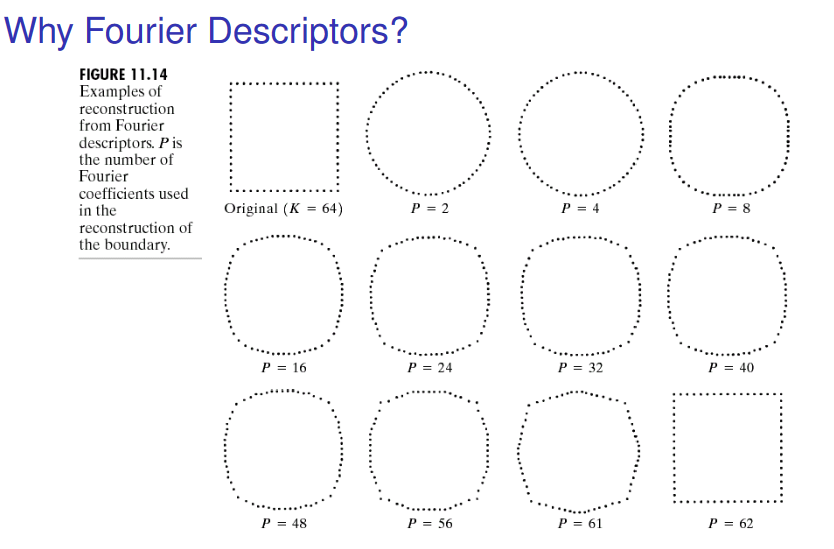
\includegraphics[width=\textwidth]{images/m2_fourier_descriptors_reconstruction.png}
    \caption{Fourier descriptor reconstruction with increasing coefficients $P$: starting from only $P=2$ coefficients (rough oval), adding more coefficients progressively recovers the detail of the original boundary ($K=64$). This demonstrates the frequency-to-detail relationship: low-$P$ = coarse shape; high-$P$ = fine shape. (Source: CV Module 2, Slide 33)}
    \label{fig:m2_fourier_recon}
\end{figure}

\subsubsection{Geometric Border Representation and B-Splines}

\textbf{Geometric Border Representation}: Represents the boundary using geometry (ordered points, straight lines, or curves) instead of pixel directions.
\begin{itemize}
    \item \textbf{Pros}: More precise than chain codes; easy to compute length, angle, curvature.
    \item \textbf{Limitation}: Sensitive to noise and small boundary changes.
\end{itemize}

\begin{figure}[H]
    \centering
    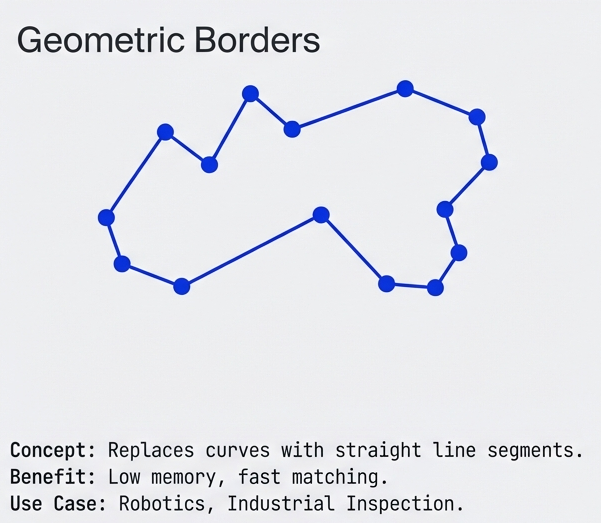
\includegraphics[width=0.65\textwidth]{images/m2_geometric_borders.png}
    \caption{Geometric border representation: the shape boundary is approximated by connecting sampled control points with straight line segments. Concept: replaces curves with line segments; benefit: low memory, fast matching; use case: robotics and industrial inspection. (Source: CV Module 2, Slide 37)}
    \label{fig:m2_geom_borders}
\end{figure}

\textbf{B-Spline Representation}: Uses smooth polynomial curves (B-splines) to model boundaries, giving a compact and smooth shape description.
\begin{itemize}
    \item A few control points define the entire smooth shape.
    \item Boundary does not pass through all points --- it is smoother.
    \item \textbf{Advantages}: Smooth; compact representation; stable under small noise.
\end{itemize}

\begin{figure}[H]
    \centering
    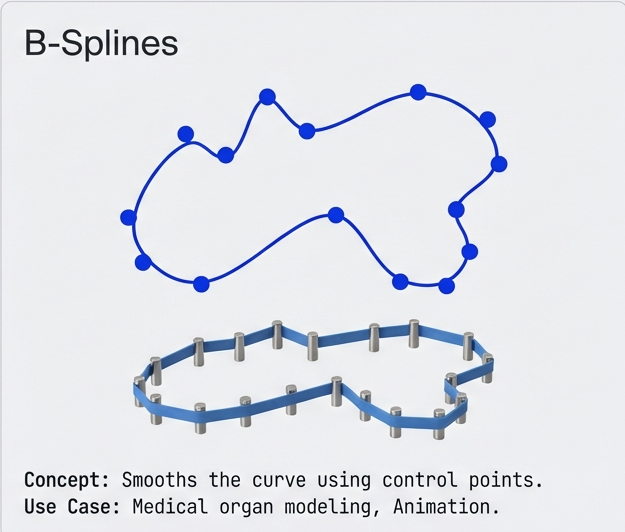
\includegraphics[width=0.65\textwidth]{images/m2_bspline_representation.png}
    \caption{B-Spline boundary representation: the shape boundary (top) is smoothed through control points via B-spline curves; the physical analogy (bottom) is a thin flexible rod (spline) constrained by pins. Concept: smooths the curve using control points; use case: medical organ modelling and animation. (Source: CV Module 2, Slide 38)}
    \label{fig:m2_bspline}
\end{figure}

\subsubsection{Shape Invariants}

Numerical features of a shape that remain unchanged under rotation, scaling, and translation. Same object looks different to a computer when rotated or resized, so invariants are essential for reliable recognition.

\textbf{Examples}: Normalized chain codes, compactness, aspect ratio, circularity.

\subsection{Region-Based Shape Representation}

Instead of describing shapes using only boundaries, region-based methods describe shapes using all pixels inside the object.

\subsubsection{Scalar Region Descriptors}

Simple numbers used to describe a region (object) in an image:
\begin{itemize}
    \item \textbf{Area}: How big the region is.
    \item \textbf{Perimeter}: Length of its boundary.
    \item \textbf{Centroid}: Center point of the region.
    \item \textbf{Compactness}: How circular or spread out it is.
    \item \textbf{Aspect Ratio}: Width vs height.
\end{itemize}

\textbf{Example}: Classifying objects (coin vs button) using area and compactness.

\begin{figure}[H]
    \centering
    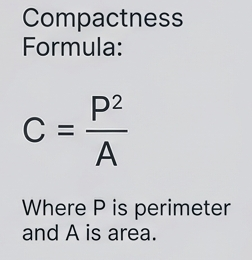
\includegraphics[width=0.35\textwidth]{images/m2_compactness_formula.png}
    \caption{Compactness formula: $C = P^2 / A$ where $P$ is the perimeter and $A$ is the area. A perfect circle has minimum compactness; elongated or irregular shapes have higher compactness values. Used as a shape invariant in region-based classification. (Source: CV Module 2, Slide 45)}
    \label{fig:m2_compactness}
\end{figure}

\subsubsection{Moments}

Statistical measures capturing shape and spatial distribution of a region. Moments encode position + spread of pixels.

\textbf{Zeroth moment} ($m_{00}$): Total mass/area of the region.

\textbf{First-order moments} ($m_{10}, m_{01}$): Center of mass (centroid).

\textbf{Second-order moments}: Spread of the region (covariance).

\textbf{Central moments} (subtracting centroid) are translation invariant. Normalized moments are scale invariant.

\subsubsection{Convex Hull}

The smallest convex shape that fully encloses a region. Imagine stretching a rubber band around an object --- the shape formed is its convex hull.

\textbf{Uses}: Measuring object solidity, hand gesture analysis.

\begin{figure}[H]
    \centering
    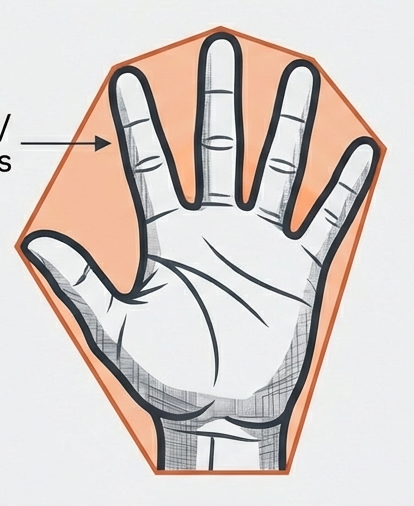
\includegraphics[width=0.5\textwidth]{images/m2_convex_hull_hand.png}
    \caption{Convex hull of a hand: the orange polygon is the tightest convex envelope around the hand outline. The concavities between fingers are ``hull defects'' and are used in finger-counting and gesture recognition algorithms. (Source: CV Module 2, Slide 48)}
    \label{fig:m2_convex_hull}
\end{figure}

\subsubsection{Region Skeletons}

A thin version of the region that preserves shape and topology. Reduces data while keeping important structure.

\textbf{Uses}: Shape recognition, medical image analysis (blood vessels, bones).

\begin{figure}[H]
    \centering
    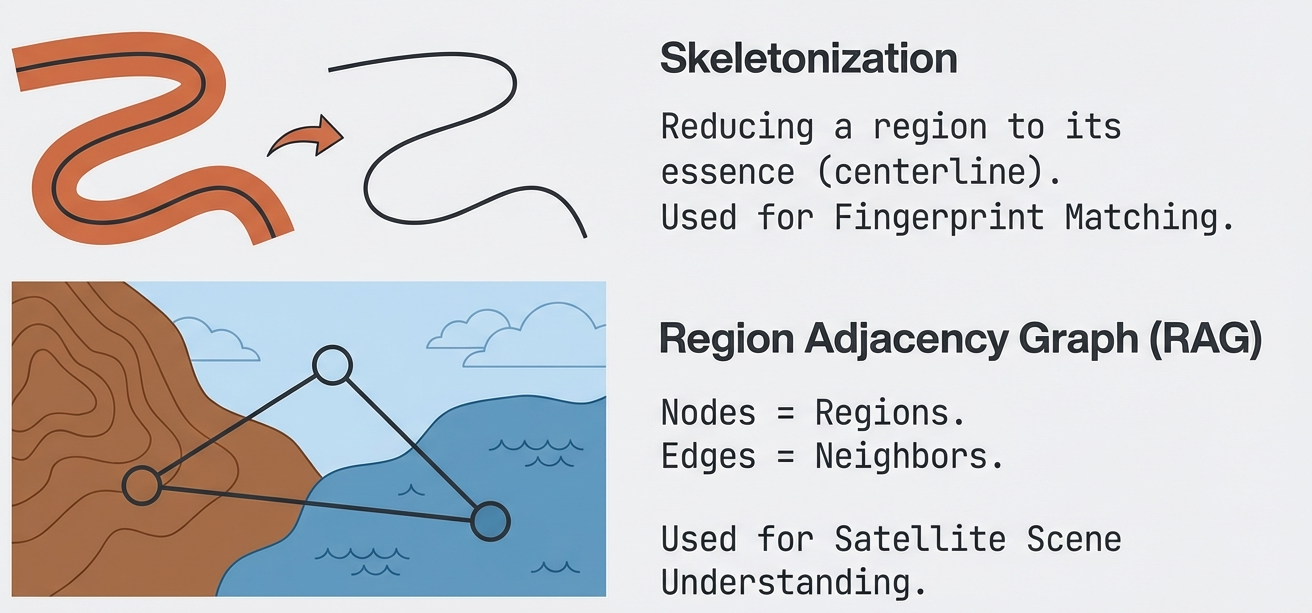
\includegraphics[width=0.85\textwidth]{images/m2_skeleton_rag.png}
    \caption{Region skeletonization (top): an S-shaped thick region is reduced to its one-pixel-wide medial axis (centerline) while preserving topology --- used for fingerprint matching. Region Adjacency Graph / RAG (bottom): a landscape image divided into land, sea, and sky regions is represented as a graph where nodes are regions and edges connect adjacent neighbours --- used for satellite scene understanding. (Source: CV Module 2, Slide 50)}
    \label{fig:m2_skeleton_rag}
\end{figure}

\subsubsection{Region Decomposition}

Dividing a large region into smaller, meaningful sub-regions. Each sub-region is more uniform, making analysis easier.

\textbf{Example}: A face image divided into eyes, nose, and mouth regions.

\subsubsection{Region Neighborhood Graph (RNG)}

Represents spatial relationships between regions using a graph:
\begin{itemize}
    \item Each region = node
    \item Adjacent regions = edges
    \item Shows which regions are neighbors
\end{itemize}

\textbf{Uses}: Scene analysis, understanding object relationships.

\begin{figure}[H]
    \centering
    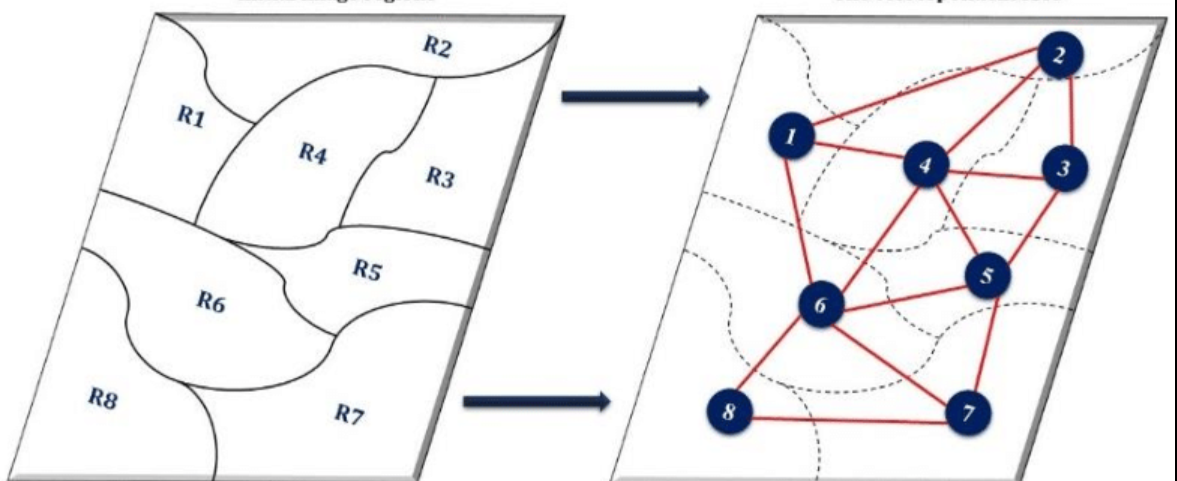
\includegraphics[width=0.85\textwidth]{images/m2_region_neighborhood_graph.png}
    \caption{Region Neighborhood Graph (RNG): an image segmented into 8 regions (R1--R8, left) is converted to a graph (right) where each node represents a region and each red edge connects two spatially adjacent regions. This structure enables scene-level reasoning about spatial relationships between objects. (Source: CV Module 2, Slide 54)}
    \label{fig:m2_rng}
\end{figure}

\subsection{Thresholding and Segmentation}

\subsubsection{Thresholding}

\textbf{Thresholding} is a segmentation technique that converts a grayscale image into a binary image by comparing each pixel intensity with a threshold value $T$:
\begin{itemize}
    \item If pixel value $\geq T \to$ object (foreground)
    \item If pixel value $< T \to$ background
\end{itemize}

\textbf{Basic Principle}: Thresholding assumes that object and background have different gray-level intensities. The pixel intensity histogram helps in selecting a threshold (two peaks = one for object, one for background; threshold lies between peaks).

\textbf{Role of Illumination}: Thresholding works best when illumination is uniform. Uneven lighting causes wrong segmentation; shadows cause misclassification.

\textbf{Solutions for Uneven Illumination}:
\begin{enumerate}
    \item \textbf{Illumination Normalization}: Reduces the effect of uneven lighting.
    \item \textbf{Retinex}: An image processing theory used to reduce illumination effects and enhance object details.
    \item \textbf{Log Transformation}: Compresses high intensity values; enhances dark regions.
    \item \textbf{Histogram Equalization}: Improves overall image contrast; spreads gray levels uniformly.
    \item \textbf{Adaptive (Local) Thresholding}: Computes threshold locally for each region; handles shadows and brightness variations.
    \item \textbf{Mean-based Local Thresholding}: Threshold is calculated using the mean intensity of a local window.
\end{enumerate}

\begin{figure}[H]
    \centering
    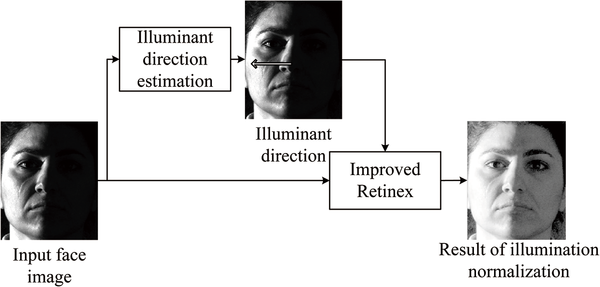
\includegraphics[width=0.85\textwidth]{images/m2_illumination_normalization.png}
    \caption{Illumination normalization pipeline for face images: an input face under uneven lighting is processed by an illuminant direction estimation block, which feeds into an Improved Retinex algorithm to produce a normalized output face with balanced illumination. This is a key preprocessing step before thresholding or segmentation. (Source: CV Module 2, Slide 61)}
    \label{fig:m2_illum_norm}
\end{figure}

\subsubsection{Global Thresholding (Iterative Method)}

Algorithm:
\begin{enumerate}
    \item Choose an initial threshold $T$.
    \item Segment the image using $T$.
    \item Compute the mean intensity of object and background.
    \item Update $T = (\text{Object mean} + \text{Background mean}) / 2$.
    \item Repeat until $T$ does not change.
\end{enumerate}

\begin{tcolorbox}[colback=yellow!5!white,colframe=yellow!75!black,title=\textbf{Worked Example 6: Iterative Global Thresholding}]
\textbf{Given}: Grayscale pixel values: 15, 20, 25, 30, 180, 190, 200, 210

\textbf{Initial threshold}: $T_0 = 100$

\textbf{Iteration 1}:
\begin{itemize}
    \item Background ($< 100$): 15, 20, 25, 30. Mean = $(15+20+25+30)/4 = 22.5$
    \item Object ($\geq 100$): 180, 190, 200, 210. Mean = $(180+190+200+210)/4 = 195$
    \item New $T = (22.5 + 195) / 2 = 108.75$
\end{itemize}

\textbf{Iteration 2}:
\begin{itemize}
    \item Background ($< 108.75$): 15, 20, 25, 30. Mean = 22.5
    \item Object ($\geq 108.75$): 180, 190, 200, 210. Mean = 195
    \item New $T = (22.5 + 195) / 2 = 108.75$ (no change)
\end{itemize}

\textbf{Final Threshold}: $T = 108.75$
\end{tcolorbox}

\subsubsection{Otsu's Method}

An automatic global thresholding method that chooses the threshold that minimizes intra-class variance (or maximizes inter-class variance).

\textbf{Intra-class variance}: How much pixel values vary within the same class. Small variance $\to$ pixels are similar $\to$ good segmentation.

\textbf{Algorithm}:
\begin{enumerate}
    \item For each possible threshold $T$: divide pixels into background and foreground.
    \item Compute mean and variance of each class.
    \item Compute weighted intra-class variance (variance $\times$ number of pixels in that class).
    \item Choose $T$ with minimum weighted variance.
\end{enumerate}

\begin{tcolorbox}[colback=yellow!5!white,colframe=yellow!75!black,title=\textbf{Worked Example 7: Otsu's Method}]
\textbf{Given}: Pixels (grayscale values): [10, 12, 14, 50, 52, 55]

\textbf{Test}: $T = 20$

\textbf{Background} = [10, 12, 14]; \textbf{Foreground} = [50, 52, 55]

\textbf{Means}:
\[
\mu_1 = (10+12+14)/3 = 12, \quad \mu_2 = (50+52+55)/3 \approx 52.3
\]

\textbf{Variances}:
\[
\sigma_1^2 = [(10-12)^2 + (12-12)^2 + (14-12)^2]/3 = (4+0+4)/3 \approx 2.67
\]
\[
\sigma_2^2 = [(50-52.3)^2 + (52-52.3)^2 + (55-52.3)^2]/3 \approx 4.22
\]

\textbf{Weighted variance}: $3 \times 2.67 + 3 \times 4.22 = 20.67$

Testing $T = 13$ gives much larger variance ($\approx 1428.8$), so $T \approx 20$ is best.
\end{tcolorbox}

\subsection{Region-Based Segmentation}

\subsubsection{Region Growing}

Start from a seed pixel and grow the region by adding similar neighboring pixels.
\begin{enumerate}
    \item Select seed point.
    \item Check neighbors.
    \item Add similar pixels.
    \item Stop when no more pixels match.
\end{enumerate}

\textbf{Example}: Tumor region detection starting from a seed pixel.

\begin{figure}[H]
    \centering
    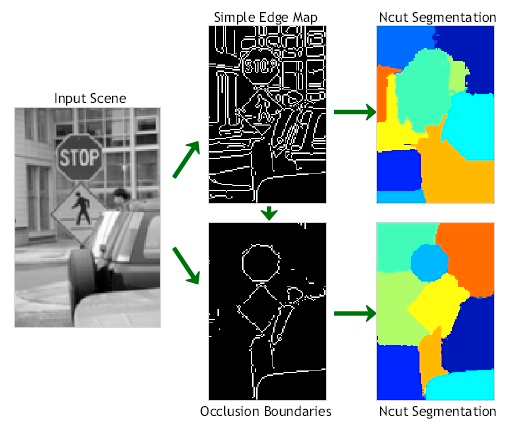
\includegraphics[width=0.85\textwidth]{images/m2_segmentation_pipeline.png}
    \caption{Image segmentation pipeline: input scene (top-left) is processed through two paths --- simple edge map (top-middle) or occlusion-boundary-aware edge map (bottom-middle) --- each fed into Normalized Cuts (Ncut) segmentation to produce colour-labelled region maps. The occlusion-aware path gives more semantically correct regions. (Source: CV Module 2, Slide 12)}
    \label{fig:m2_seg_pipeline}
\end{figure}

\subsubsection{Region Splitting and Merging}

\textbf{Region Splitting}: Divide image into smaller regions until uniformity is satisfied.

\textbf{Region Merging}: Merge adjacent regions if they are similar.

\textbf{Why both?}: Imagine an image with forest, water, and urban area. Initially the entire image is not uniform, so split until regions have similar texture. After splitting, many small regions have the same texture, so merge neighboring regions with similar texture.

\subsection{Pixel Connectivity}

Defines how pixels are connected in an image. Understanding connectivity is critical for region growing, connected component labelling, and contour tracing algorithms.
\begin{enumerate}
    \item \textbf{4-connectivity}: Pixels are connected if they share an edge (up, down, left, right).
    \item \textbf{8-connectivity}: Pixels are connected if they share an edge or corner (includes diagonals).
    \item \textbf{m-connectivity} (mixed): Diagonal connection is allowed only if there is no 4-connected side path between the pixels. Prevents false merging when objects touch only at corners.
\end{enumerate}

\textbf{Example}:
\[
\begin{bmatrix} 1 & 1 & . & . \\ 1 & 1 & . & . \\ . & . & 1 & 1 \\ . & . & 1 & 1 \end{bmatrix}
\]

Two blocks of 1s touch only at corners. Under 4-connectivity they are separate; under 8-connectivity they are connected; under m-connectivity they are separate (no side path exists).

\begin{figure}[H]
    \centering
    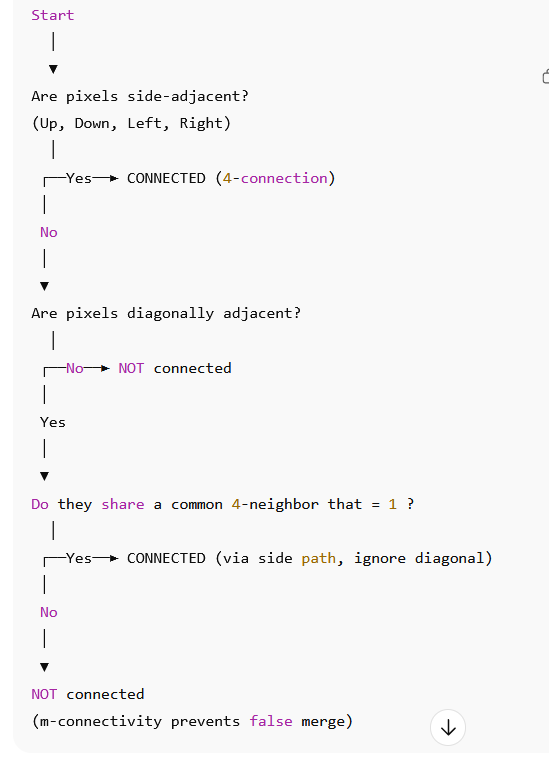
\includegraphics[width=0.6\textwidth]{images/m2_pixel_connectivity_flowchart.png}
    \caption{Pixel connectivity decision flowchart: given two pixels, first check 4-connectivity (side-adjacent $\to$ connected); if not, check diagonal adjacency; if diagonal and they share a common 4-neighbour with value 1, they are m-connected (avoids false diagonal merges); otherwise not connected. (Source: CV Module 2, Slide 81)}
    \label{fig:m2_pixel_conn}
\end{figure}

\subsection{Hough Transform}

A technique used to detect geometric shapes (lines, circles, ellipses) in images even if edges are broken or noisy.

\textbf{Traditional edge detection} gives points, not shapes. The Hough Transform converts edge points into parameter space where each point ``votes'' for possible lines. The line that gets the most votes is detected as the real line.

\textbf{Example}: In a road image, many white lane pixels lie in a line. The Hough Transform detects that line as the lane marking.

\begin{tcolorbox}[colback=yellow!5!white,colframe=yellow!75!black,title=\textbf{Worked Example 8: Hough Transform Line Detection}]
\textbf{Given}: Three edge points: $(1, 1)$, $(2, 2)$, $(3, 3)$.

\textbf{Step 1}: Convert each point to parameter space using $y = mx + c \to c = -xm + y$.
\begin{itemize}
    \item For $(1, 1)$: $c = -m + 1$ (line in parameter space)
    \item For $(2, 2)$: $c = -2m + 2$ (line in parameter space)
    \item For $(3, 3)$: $c = -3m + 3$ (line in parameter space)
\end{itemize}

\textbf{Step 2}: Find intersection in parameter space. All three lines intersect at $m = 1, c = 0$.

\textbf{Step 3}: The detected line is $y = x$.

\textbf{Interpretation}: Even if some edge points are missing, the Hough Transform can still detect the line from the remaining points.
\end{tcolorbox}

\newpage

\section{Module 3: Object Detection and Convolutional Neural Networks}

\subsection{Introduction to Object Detection}

\textbf{Object detection} identifies what objects are present and where they are located in an image by predicting class labels + bounding box coordinates. Detection = classification + localization.

\textbf{The Human Brain Detects Objects}:
\begin{enumerate}
    \item \textbf{Light and Eye Perception}: Captures visual input.
    \item \textbf{Feature Detection}: V1 (Primary Visual Cortex) detects edges, lines, and colors; V4 \& IT Cortex recognize shapes, textures, patterns.
    \item \textbf{Object Recognition (Top-Down Processing)}: Brain matches visual input with stored memories; uses context and past experiences to interpret objects.
\end{enumerate}

\textbf{How Do Computers Detect Objects?}:
\begin{enumerate}
    \item \textbf{Image Preprocessing}: Convert image into pixels (grayscale/RGB); apply filters (edge detection, etc.).
    \item \textbf{Feature Extraction}: Deep Learning (CNNs) extracts patterns hierarchically.
    \item \textbf{Object Detection Methods}: Sliding Window, R-CNN family, YOLO (You Only Look Once), SSD, DETR.
\end{enumerate}

\begin{figure}[H]
    \centering
    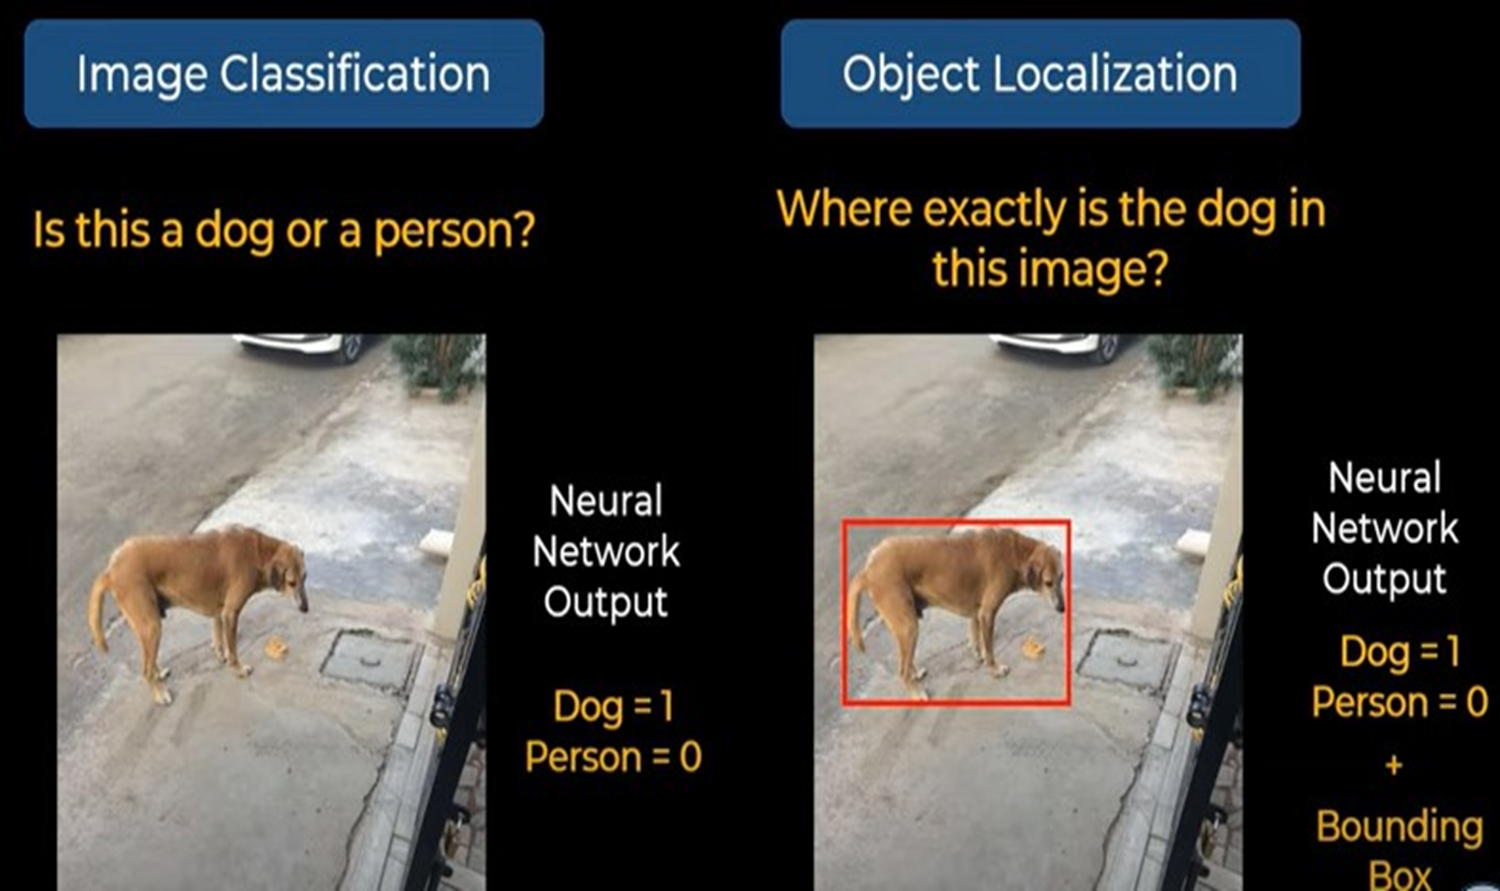
\includegraphics[width=0.85\textwidth]{images/m3_classification_vs_localization.png}
    \caption{Image Classification vs.~Object Localization: Classification (left) answers ``Is this a dog?'' and outputs a class label; Localization (right) answers ``Where is the dog?'' and outputs class label plus a bounding box. Detection extends localization to multiple objects. (Source: CV Module 3)}
    \label{fig:m3_cls_vs_loc}
\end{figure}

\subsection{Types of Object Detection}

\subsubsection{Two-Stage Object Detection (Region Proposal-Based)}

\textbf{Stage 1 -- Region Proposal}: The model first generates potential object regions using algorithms like Selective Search or Region Proposal Networks (RPNs).

\textbf{Stage 2 -- Classification \& Refinement}: Each proposed region is classified and refined to improve accuracy.

\textbf{Advantages}: High accuracy due to separate proposal and classification stages; handles small and overlapping objects better.

\textbf{Disadvantages}: Slower because of the extra proposal step; not ideal for real-time applications.

\textbf{Examples}: R-CNN, Fast R-CNN, Faster R-CNN.

\subsubsection{One-Stage Object Detection (End-to-End, No Proposals)}

The model directly predicts object locations and classes in one pass without a separate region proposal step.

\textbf{Advantages}: Much faster --- ideal for real-time applications; simpler architecture.

\textbf{Disadvantages}: Slightly lower accuracy than two-stage methods, especially for small objects; more false positives due to direct prediction.

\textbf{Examples}: YOLO (You Only Look Once), SSD (Single Shot MultiBox Detector), RetinaNet.

\subsubsection{Proposal-Free / Transformer-Based Detection}

Completely avoids region proposal mechanisms. Uses transformer-based architectures.

\textbf{Advantages}: Most efficient --- eliminates proposal generation completely; scales better for large datasets.

\textbf{Disadvantages}: Still evolving --- accuracy improvements are ongoing; some methods require huge computational power.

\textbf{Examples}: DETR (DEtection TRansformer), Vision Transformers (ViTs) in object detection.

\begin{tcolorbox}[colback=green!5!white,colframe=green!75!black,title=\textbf{Worked Example 9: Two-Stage vs One-Stage Comparison}]
\textbf{Scenario}: A self-driving car must detect pedestrians in real time.

\textbf{Two-Stage (Faster R-CNN)}:
\begin{itemize}
    \item RPN generates ~2000 region proposals per image.
    \item Each proposal is classified and refined.
    \item Time: ~200ms per image (5 FPS).
    \item Accuracy: High (mAP ~75\%).
    \item \textbf{Verdict}: Too slow for real-time driving decisions.
\end{itemize}

\textbf{One-Stage (YOLOv8)}:
\begin{itemize}
    \item Image divided into $19 \times 19$ grid; each cell predicts directly.
    \item Time: ~10ms per image (100 FPS).
    \item Accuracy: Good (mAP ~65\%).
    \item \textbf{Verdict}: Fast enough for real-time; acceptable accuracy trade-off.
\end{itemize}

\textbf{Conclusion}: For safety-critical real-time applications, one-stage detectors are preferred despite slightly lower accuracy.
\end{tcolorbox}

\subsection{R-CNN Family}

\subsubsection{R-CNN (Region-based CNN)}

\textbf{Process}:
\begin{enumerate}
    \item Use Selective Search to generate ~2000 region proposals.
    \item Warp each region to fixed size ($227 \times 227$).
    \item Pass through CNN to extract features.
    \item Use SVM for classification and linear regression for bounding box refinement.
\end{enumerate}

\textbf{Problem}: Each proposal is processed independently --- very slow.

\begin{figure}[H]
    \centering
    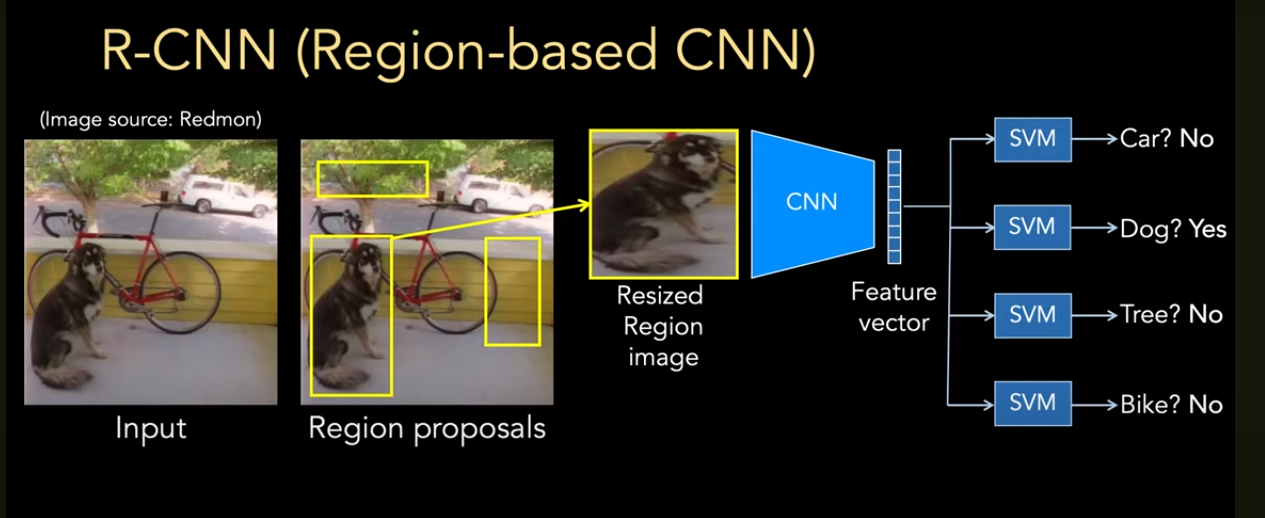
\includegraphics[width=0.85\textwidth]{images/m3_rcnn_pipeline.png}
    \caption{R-CNN (Region-based CNN) Pipeline: Input image $\to$ Selective Search generates ~2000 region proposals $\to$ each proposal is resized and passed individually through a CNN $\to$ feature vector fed into SVMs for classification (Car? Dog? Bike?) and linear regression for bounding box refinement. (Source: CV Module 3)}
    \label{fig:m3_rcnn}
\end{figure}

\begin{figure}[H]
    \centering
    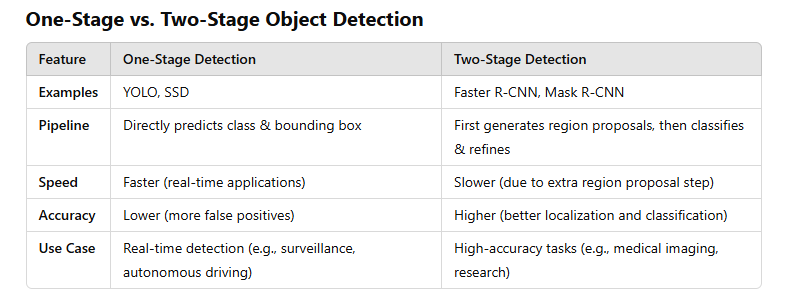
\includegraphics[width=0.85\textwidth]{images/m3_one_vs_two_stage_table.png}
    \caption{One-Stage vs.~Two-Stage Object Detection comparison: Two-stage (Faster R-CNN, Mask R-CNN) achieves higher accuracy via a separate proposal step; one-stage (YOLO, SSD) is faster and suited for real-time use. (Source: CV Module 3)}
    \label{fig:m3_stage_compare}
\end{figure}

\subsubsection{Fast R-CNN}

\textbf{Improvement}: Instead of processing each proposal separately, the entire image is passed through the CNN once to get a feature map. Region proposals are then projected onto this feature map.

\textbf{Process}:
\begin{enumerate}
    \item Pass entire image through CNN to get feature map.
    \item Project region proposals onto feature map (RoI pooling).
    \item Use fully connected layers for classification and bounding box regression.
\end{enumerate}

\textbf{Speedup}: ~10x faster than R-CNN.

\begin{figure}[H]
    \centering
    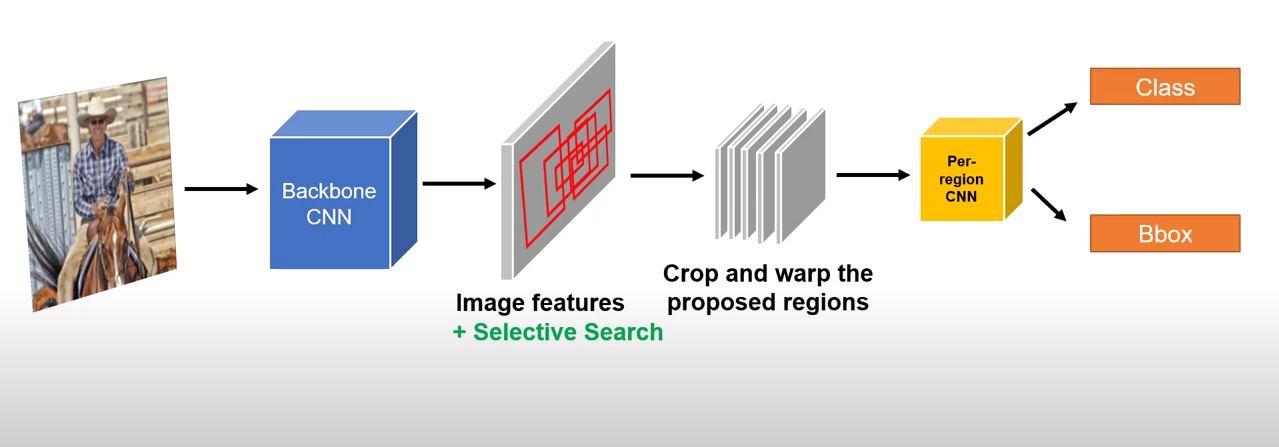
\includegraphics[width=0.85\textwidth]{images/m3_fast_rcnn_pipeline.png}
    \caption{Fast R-CNN Pipeline: The entire image is passed once through a Backbone CNN (e.g., VGG) to produce a shared feature map; Selective Search proposals are projected onto this map; RoI Pooling extracts fixed $7\times7$ features per region; two FC layers produce class scores and bounding box offsets in parallel. (Source: CV Module 3)}
    \label{fig:m3_fast_rcnn}
\end{figure}

\subsubsection{Faster R-CNN}

\textbf{Improvement}: Replaces Selective Search with a \textbf{Region Proposal Network (RPN)} that shares convolutional features with the detection network.

\textbf{Process}:
\begin{enumerate}
    \item CNN backbone extracts features from the entire image.
    \item \textbf{RPN} slides a small network over the feature map to generate region proposals.
    \item RoI pooling extracts fixed-size features from each proposal.
    \item Classification + bounding box regression.
\end{enumerate}

\textbf{Speedup}: ~250x faster than R-CNN; nearly real-time.

\begin{figure}[H]
    \centering
    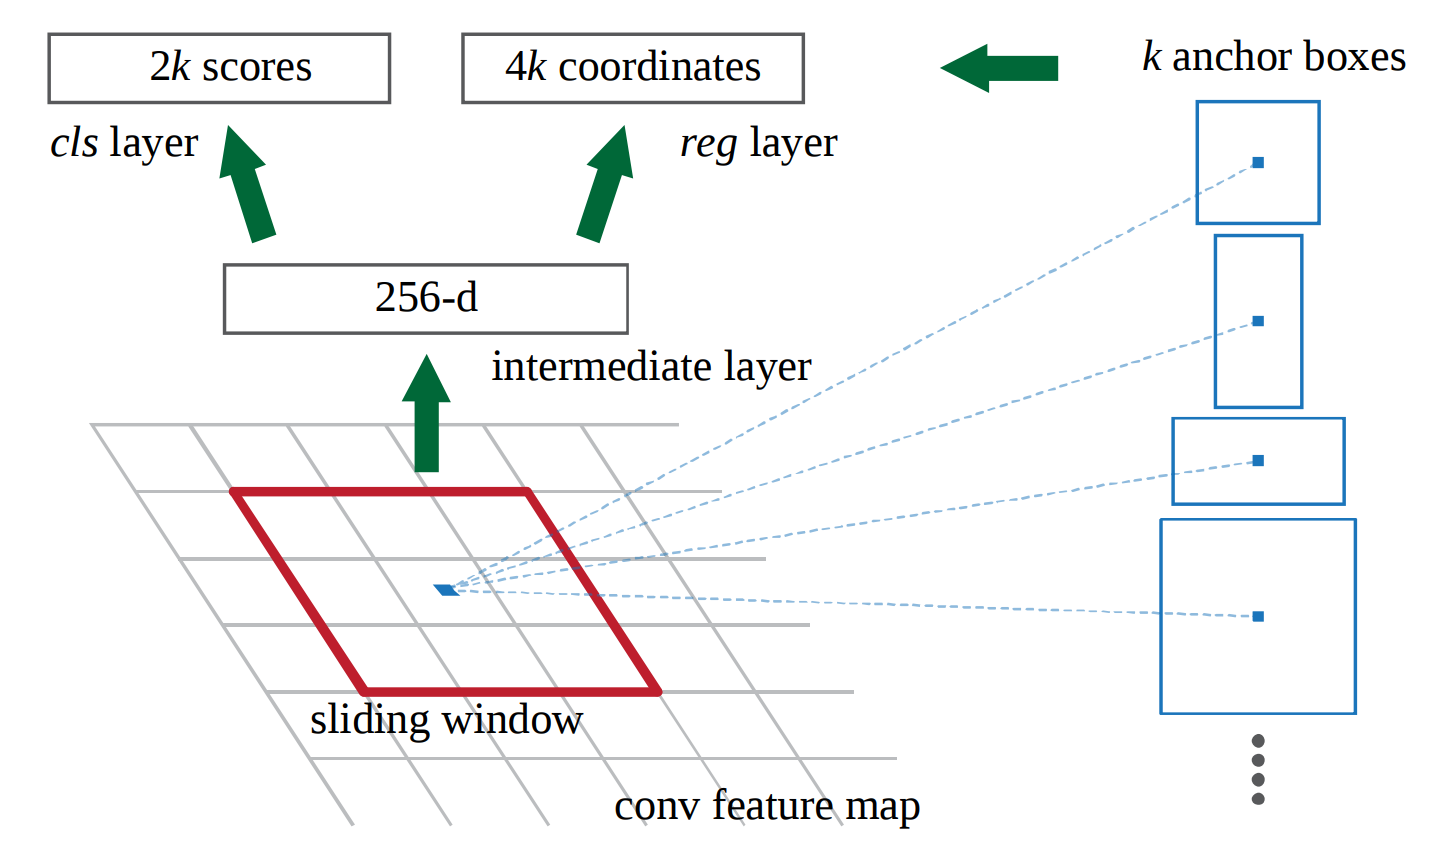
\includegraphics[width=0.85\textwidth]{images/m3_rpn_arch.png}
    \caption{Region Proposal Network (RPN): A $3\times3$ sliding window sweeps the conv feature map; for each position, $k$ anchor boxes of varying scales/ratios are evaluated. A 256-d intermediate layer feeds into two heads: \textit{cls} layer ($2k$ objectness scores: object/background) and \textit{reg} layer ($4k$ box-regression coordinates). NMS retains top proposals. (Source: CV Module 3)}
    \label{fig:m3_rpn}
\end{figure}

\begin{figure}[H]
    \centering
    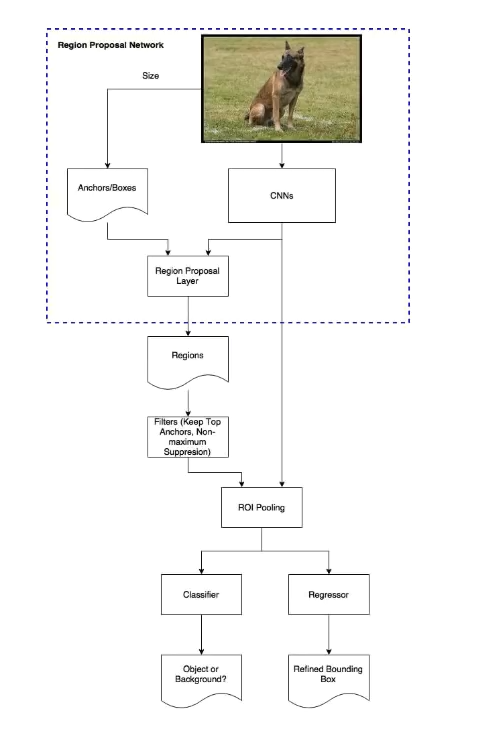
\includegraphics[width=0.85\textwidth]{images/m3_rpn_flowchart.png}
    \caption{Faster R-CNN full workflow: RPN takes anchors and CNN features $\to$ Region Proposal Layer $\to$ NMS filters top anchors $\to$ RoI Pooling $\to$ parallel Classifier (object or background?) and Regressor (refined bounding box). (Source: CV Module 3)}
    \label{fig:m3_faster_rcnn}
\end{figure}

\begin{figure}[H]
    \centering
    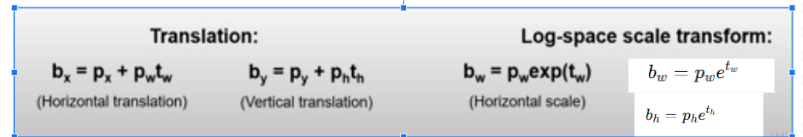
\includegraphics[width=0.85\textwidth]{images/m3_bbox_transform_formulas.png}
    \caption{Bounding Box Regression Transform: Given a region proposal $(p_x,p_y,p_h,p_w)$, the network predicts transforms $(t_x,t_y,t_h,t_w)$. Translation: $b_x = p_x + p_w t_w$, $b_y = p_y + p_h t_h$. Log-space scale: $b_w = p_w e^{t_w}$, $b_h = p_h e^{t_h}$. (Source: CV Module 3)}
    \label{fig:m3_bbox_transform}
\end{figure}

\begin{center}
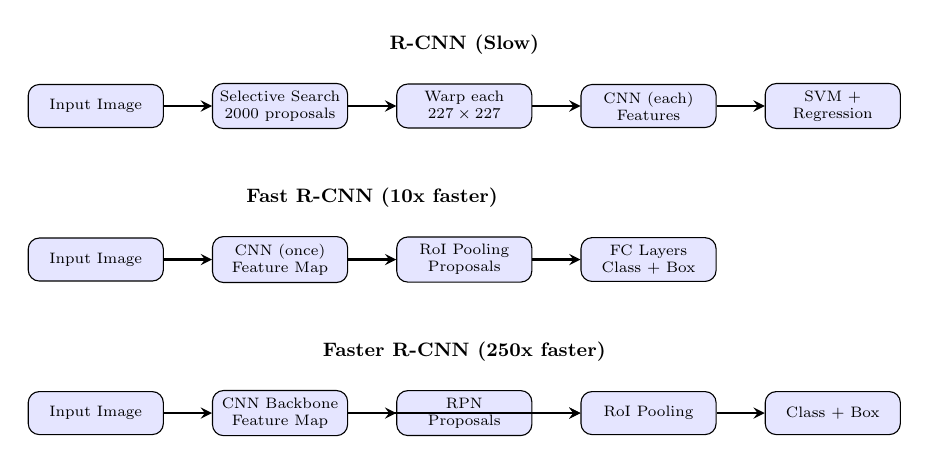
\begin{tikzpicture}[scale=0.78, every node/.style={scale=0.78},
    node distance=1.5cm,
    box/.style={rectangle, draw, rounded corners, minimum width=2.2cm, minimum height=0.7cm, font=\scriptsize, align=center, fill=blue!10},
    arrow/.style={->, >=stealth, thick}
]
% R-CNN
\node[box] (input1) at (0,0) {Input Image};
\node[box] (ss1) at (3,0) {Selective Search\\2000 proposals};
\node[box] (warp1) at (6,0) {Warp each\\$227\times227$};
\node[box] (cnn1) at (9,0) {CNN (each)\\Features};
\node[box] (svm1) at (12,0) {SVM +\\Regression};
\draw[arrow] (input1) -- (ss1);
\draw[arrow] (ss1) -- (warp1);
\draw[arrow] (warp1) -- (cnn1);
\draw[arrow] (cnn1) -- (svm1);
\node[font=\small\bfseries] at (6, 1) {R-CNN (Slow)};

% Fast R-CNN
\node[box] (input2) at (0,-2.5) {Input Image};
\node[box] (cnn2) at (3,-2.5) {CNN (once)\\Feature Map};
\node[box] (ss2) at (6,-2.5) {RoI Pooling\\Proposals};
\node[box] (fc2) at (9,-2.5) {FC Layers\\Class + Box};
\draw[arrow] (input2) -- (cnn2);
\draw[arrow] (cnn2) -- (ss2);
\draw[arrow] (ss2) -- (fc2);
\node[font=\small\bfseries] at (4.5, -1.5) {Fast R-CNN (10x faster)};

% Faster R-CNN
\node[box] (input3) at (0,-5) {Input Image};
\node[box] (cnn3) at (3,-5) {CNN Backbone\\Feature Map};
\node[box] (rpn3) at (6,-5) {RPN\\Proposals};
\node[box] (roi3) at (9,-5) {RoI Pooling};
\node[box] (fc3) at (12,-5) {Class + Box};
\draw[arrow] (input3) -- (cnn3);
\draw[arrow] (cnn3) -- (rpn3);
\draw[arrow] (rpn3) -- (roi3);
\draw[arrow] (cnn3) -- (roi3);
\draw[arrow] (roi3) -- (fc3);
\node[font=\small\bfseries] at (6, -4) {Faster R-CNN (250x faster)};

\end{tikzpicture}
\end{center}
\captionof{figure}{R-CNN evolution: From R-CNN (2000 separate CNN passes) to Fast R-CNN (one CNN pass + RoI pooling) to Faster R-CNN (RPN shares features with detector).}

\subsection{YOLO (You Only Look Once)}

YOLO is a one-stage detector that predicts all bounding boxes in a single forward pass. The input image is resized and divided into an $S \times S$ grid. Each grid cell is responsible for detecting objects whose center lies inside it.

\subsubsection{YOLO Grid Prediction}

Each grid cell predicts:
\begin{itemize}
    \item $B$ bounding boxes (each with 5 values: $x, y, w, h$, confidence)
    \item Class probabilities for each box
\end{itemize}

\textbf{Coordinate system}:
\begin{itemize}
    \item $x, y$: Box center coordinates relative to grid cell (0--1).
    \item $w, h$: Width and height relative to full image (0--1).
    \item Confidence: Object present + how well the box fits.
\end{itemize}

\textbf{Output vector per grid cell}: $B \times 5 + N$ (where $N$ = number of classes).

\textbf{Example}: $B = 2$, $N = 20$ $\to$ Each grid cell outputs a 30-length vector.

\begin{center}
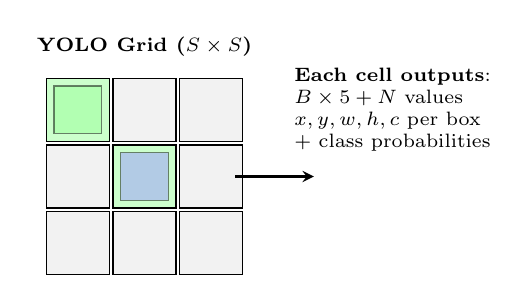
\begin{tikzpicture}[
    node distance=0.3cm,
    gridcell/.style={rectangle, draw, minimum size=0.8cm, font=\tiny},
    objcell/.style={gridcell, fill=green!20},
    emptycell/.style={gridcell, fill=gray!10},
    arrow/.style={->, >=stealth, thick}
]
% 3x3 grid
\node[objcell] at (0,0) {};
\node[emptycell] at (0.85,0) {};
\node[emptycell] at (1.7,0) {};
\node[emptycell] at (0,-0.85) {};
\node[objcell] at (0.85,-0.85) {};
\node[emptycell] at (1.7,-0.85) {};
\node[emptycell] at (0,-1.7) {};
\node[emptycell] at (0.85,-1.7) {};
\node[emptycell] at (1.7,-1.7) {};

% Object representations
\draw[fill=green!40, opacity=0.5] (-0.3,0.3) rectangle (0.3,-0.3);
\draw[fill=blue!40, opacity=0.5] (0.55,-1.15) rectangle (1.15,-0.55);

% Labels
\node[font=\scriptsize] at (0.85, 0.8) {\textbf{YOLO Grid ($S \times S$)}};
\node[font=\scriptsize, align=left] at (4, 0) {
\textbf{Each cell outputs}: \\
$B \times 5 + N$ values \\
$x, y, w, h, c$ per box \\
+ class probabilities
};

\draw[arrow] (2, -0.85) -- (3, -0.85);

\end{tikzpicture}
\end{center}
\captionof{figure}{YOLO grid-based detection: Image divided into $S \times S$ grid cells. Cells containing object centers (green) predict bounding boxes; empty cells (gray) predict background.}

\subsubsection{Anchor Boxes}

\begin{figure}[H]
    \centering
    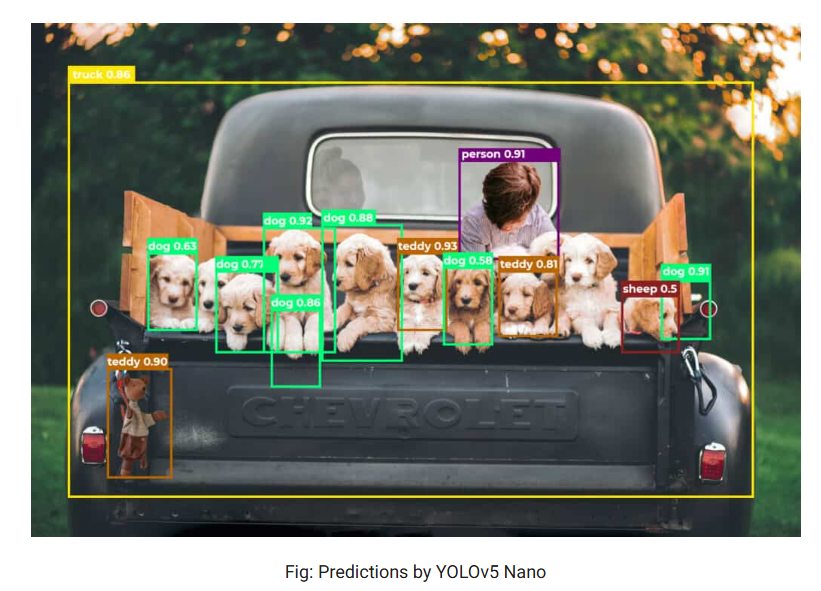
\includegraphics[width=0.85\textwidth]{images/m3_yolo_predictions.png}
    \caption{YOLO Predictions (YOLOv5 Nano): Bounding boxes with class labels and confidence scores overlaid on the input image in a single forward pass --- truck (0.98), dogs, person, teddy, sheep detected simultaneously. (Source: CV Module 3)}
    \label{fig:m3_yolo_pred}
\end{figure}

\textbf{Problem}: In YOLOv1, one grid cell = one object. If two objects have centers in the same cell, one is missed.

\textbf{Solution}: \textbf{Anchor Boxes}. Each grid cell predicts multiple bounding boxes (typically 2 to 9), each with its own confidence and class prediction.

\textbf{Anchor}: Starting box = initial guess (fixed before training).

\textbf{Bounding Box}: Final predicted box = corrected guess (predicted after training).

\textbf{Example}: If a cell has 2 anchors and 2 classes:
\begin{itemize}
    \item Anchor 1 = 7 values ($x, y, w, h, c$ + 2 classes)
    \item Anchor 2 = 7 values
    \item Total = 14 values per cell
\end{itemize}

\begin{figure}[H]
    \centering
    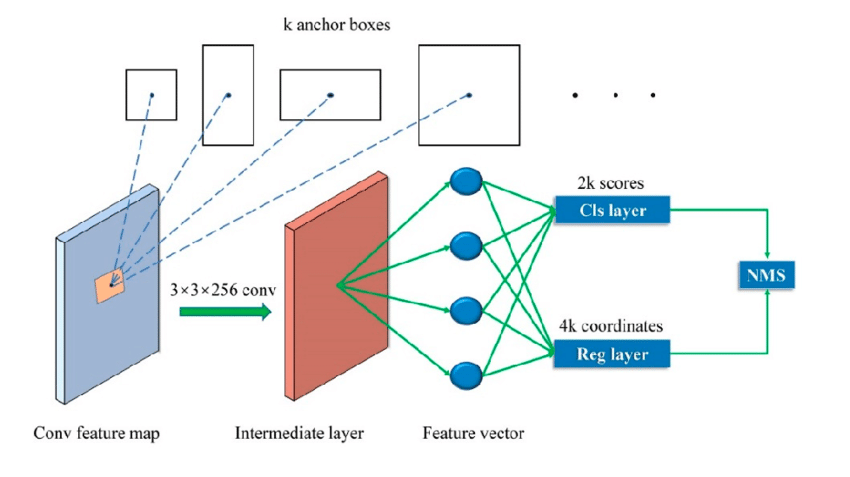
\includegraphics[width=0.85\textwidth]{images/m3_rpn_with_nms.png}
    \caption{RPN with Anchor Boxes and NMS: Conv feature map $\to$ $3\times3\times256$ conv $\to$ feature vector $\to$ cls layer outputs $2k$ objectness scores and reg layer outputs $4k$ coordinates for $k$ anchor boxes; NMS post-processes to keep top proposals. (Source: CV Module 3)}
    \label{fig:m3_rpn_nms}
\end{figure}

\subsubsection{YOLO Loss Function}

The YOLO loss function measures how well the model's predictions match the actual objects. It consists of three parts:

\begin{enumerate}
    \item \textbf{Localization Loss (Bounding Box Error)}:
    \begin{itemize}
        \item Ensures predicted bounding boxes are close to ground truth.
        \item Uses MSE on $x, y, w, h$.
        \item \textbf{Square root trick}: $\sqrt{w}$ and $\sqrt{h}$ instead of $w$ and $h$ to balance small and large objects.
    \end{itemize}

    \item \textbf{Confidence Loss (Objectness Error)}:
    \begin{itemize}
        \item Ensures the model correctly predicts if an object is present.
        \item Compares predicted confidence with actual presence (1 if object, 0 if not).
        \item \textbf{$\lambda_{\text{noobj}}$}: Reduces penalty for empty cells (typically 0.5).
    \end{itemize}

    \item \textbf{Classification Loss (Object Type Error)}:
    \begin{itemize}
        \item Ensures correct object classification.
        \item Uses cross-entropy loss between predicted and actual class labels.
    \end{itemize}
\end{enumerate}

\[
\text{Total Loss} = \lambda_{\text{coord}} \cdot \text{Localization Loss} + \lambda_{\text{obj}} \cdot \text{Confidence Loss} + \lambda_{\text{class}} \cdot \text{Classification Loss}
\]

\begin{figure}[H]
    \centering
    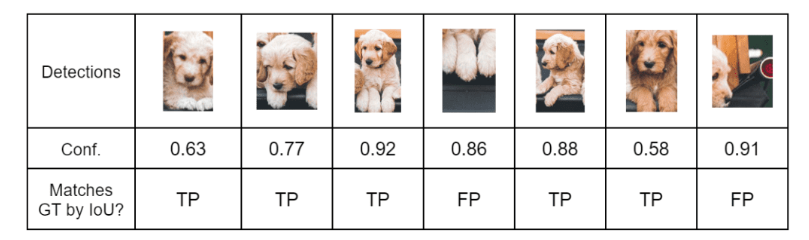
\includegraphics[width=0.85\textwidth]{images/m3_tp_fp_table.png}
    \caption{TP/FP classification table for YOLO detections: Predictions sorted by confidence; each is matched against ground truth via IoU threshold. TP = correct detection; FP = wrong detection. Used as input to compute Precision--Recall curve and mAP. (Source: CV Module 3)}
    \label{fig:m3_tp_fp}
\end{figure}

\subsubsection{YOLO Variants}

\begin{itemize}
    \item \textbf{YOLOv1 (2015)}: First version; divides image into grid; fast but less accurate for small objects.
    \item \textbf{YOLOv2 (2017)}: Added anchor boxes, batch normalization, multi-scale training.
    \item \textbf{YOLOv3 (2018)}: Feature pyramid for multi-scale detection; Darknet-53 backbone.
    \item \textbf{YOLOv4 (2020)}: CSPDarknet-53, mosaic augmentation, self-adversarial training.
    \item \textbf{YOLOv5 (2020)}: Smaller and faster; AutoAnchor optimization.
    \item \textbf{YOLOv8 (2023)}: Supports detection, segmentation, and tracking in one model.
    \item \textbf{YOLOv11 (2024)}: Pose estimation, instance segmentation, greater accuracy with fewer parameters.
\end{itemize}


\subsection{SSD (Single Shot MultiBox Detector)}

SSD is a one-stage object detector that uses multiple feature maps at different scales to detect objects of varying sizes.

\textbf{Architecture}:
\begin{enumerate}
    \item \textbf{Input}: $300 \times 300$ image.
    \item \textbf{Backbone (VGG-16)}: Extracts features (e.g., Conv4\_3 $\to$ $38 \times 38 \times 512$).
    \item \textbf{Extra Feature Layers}: Produce smaller feature maps ($19 \times 19$, $10 \times 10$, $5 \times 5$, etc.).
    \item \textbf{Prediction Layers}: Each feature map predicts bounding boxes and class probabilities using default/prior boxes.
    \item \textbf{Post-processing}: Combine predictions from all feature maps; apply NMS.
\end{enumerate}

\textbf{Key Idea}: High-resolution maps detect small objects; low-resolution maps detect large objects.


\subsection{Evaluation Metrics}

\subsubsection{IoU (Intersection over Union)}

IoU measures how well the predicted bounding box overlaps with the ground truth box:
\[
\text{IoU} = \frac{|A \cap B|}{|A \cup B|} = \frac{\text{Intersection}}{\text{Union}}
\]

Typically, IoU $> 0.5$ is considered a correct detection.

\begin{figure}[H]
    \centering
    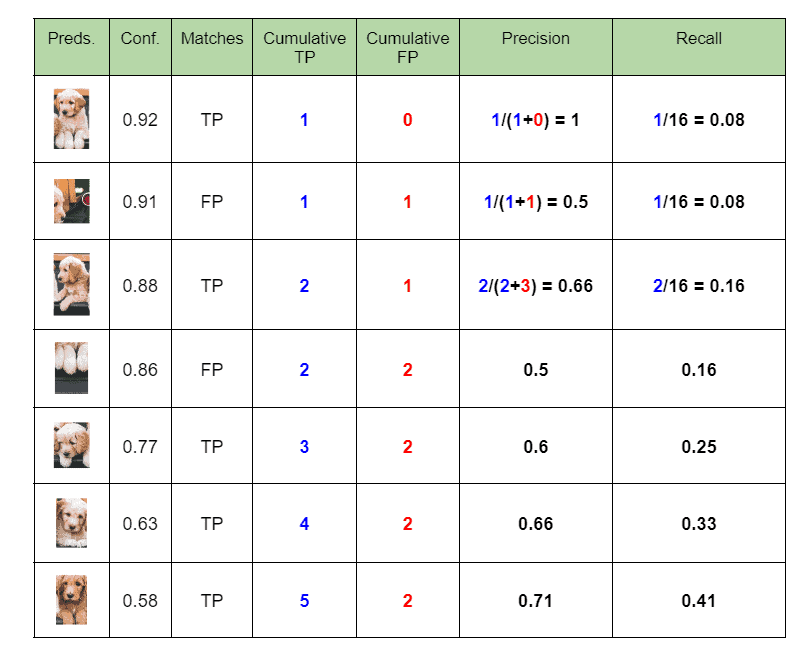
\includegraphics[width=0.85\textwidth]{images/m3_precision_recall_table.png}
    \caption{Cumulative Precision--Recall table: Detections sorted by confidence; cumulative TP and FP are tracked; Precision = TP/(TP+FP) and Recall = TP/Total GT are computed at each step to plot the Precision--Recall curve and calculate Average Precision (AP). (Source: CV Module 3)}
    \label{fig:m3_pr_table}
\end{figure}

\subsubsection{Precision and Recall}

\begin{itemize}
    \item \textbf{TP (True Positive)}: Predicted box correctly detects a real object.
    \item \textbf{FP (False Positive)}: Predicted box detects something that is not a real object.
    \item \textbf{FN (False Negative)}: Real object exists but the model failed to detect it.
\end{itemize}

\[
\text{Precision} = \frac{\text{TP}}{\text{TP} + \text{FP}}, \quad
\text{Recall} = \frac{\text{TP}}{\text{TP} + \text{FN}}
\]

\subsubsection{mAP (Mean Average Precision)}

\begin{enumerate}
    \item Sort predictions by confidence score (descending).
    \item For each prediction, compute IoU with ground truth.
    \item If IoU $\geq$ threshold $\to$ TP; else FP.
    \item After each box, calculate cumulative Precision and Recall.
    \item \textbf{AP} (Average Precision) = area under the Precision--Recall curve for one class.
    \item \textbf{mAP} = average of AP scores across all classes.
\end{enumerate}

\begin{tcolorbox}[colback=yellow!5!white,colframe=yellow!75!black,title=\textbf{Worked Example 10: IoU, Precision, Recall, and mAP}]
\textbf{Given}: An image contains 3 ground truth bicycles. A model predicts 4 bounding boxes with confidence scores: 0.95, 0.85, 0.70, 0.40. After IoU matching: Box 1 correct, Box 2 incorrect, Box 3 correct, Box 4 correct.

\textbf{Step 1 -- Cumulative TP and FP}:
\begin{itemize}
    \item After Box 1 (0.95, correct): TP=1, FP=0 $\to$ Precision=1.0, Recall=1/3=0.33
    \item After Box 2 (0.85, incorrect): TP=1, FP=1 $\to$ Precision=0.5, Recall=0.33
    \item After Box 3 (0.70, correct): TP=2, FP=1 $\to$ Precision=0.67, Recall=0.66
    \item After Box 4 (0.40, correct): TP=3, FP=1 $\to$ Precision=0.75, Recall=1.0
\end{itemize}

\textbf{Step 2 -- AP}:
\[
\text{AP} = \frac{1.0 + 0.5 + 0.67 + 0.75}{4} = 0.73
\]

\textbf{Step 3 -- mAP}: If AP for another class (bus) = 0.65:
\[
\text{mAP} = \frac{0.73 + 0.65}{2} = 0.69
\]

\textbf{Answer}: mAP = \textbf{0.69} (69\%).
\end{tcolorbox}

\subsection{Non-Maximum Suppression (NMS)}

Object detection models often predict multiple bounding boxes for the same object. NMS removes duplicates by:
\begin{enumerate}
    \item Selecting the box with the highest confidence score.
    \item Removing all other boxes of the same class with IoU $>$ threshold (typically 0.5) with the selected box.
    \item Repeating until no boxes remain.
\end{enumerate}

\textbf{When NOT to apply NMS}: If two overlapping bounding boxes refer to \textbf{different objects}, they should not be removed. In such cases, use \textbf{Soft-NMS} to reduce confidence instead of removing boxes.

\textbf{Example}: Two boxes both detect a car with IoU = 0.7 and confidence scores 0.9 and 0.6. NMS keeps the 0.9 box and removes the 0.6 box.

\begin{figure}[H]
    \centering
    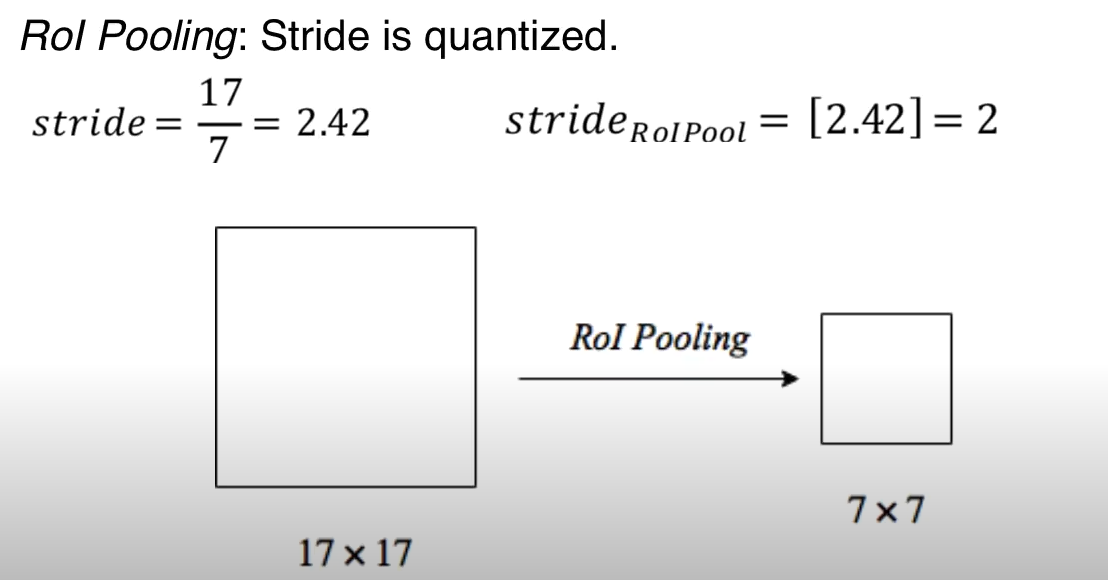
\includegraphics[width=0.85\textwidth]{images/m3_roi_pooling.png}
    \caption{RoI Pooling: A $17\times17$ feature region is quantized to stride $= \lfloor17/7\rfloor = 2$ and max-pooled to a fixed $7\times7$ output. Quantization introduces misalignment. (Source: CV Module 3)}
    \label{fig:m3_roi_pool}
\end{figure}

\begin{figure}[H]
    \centering
    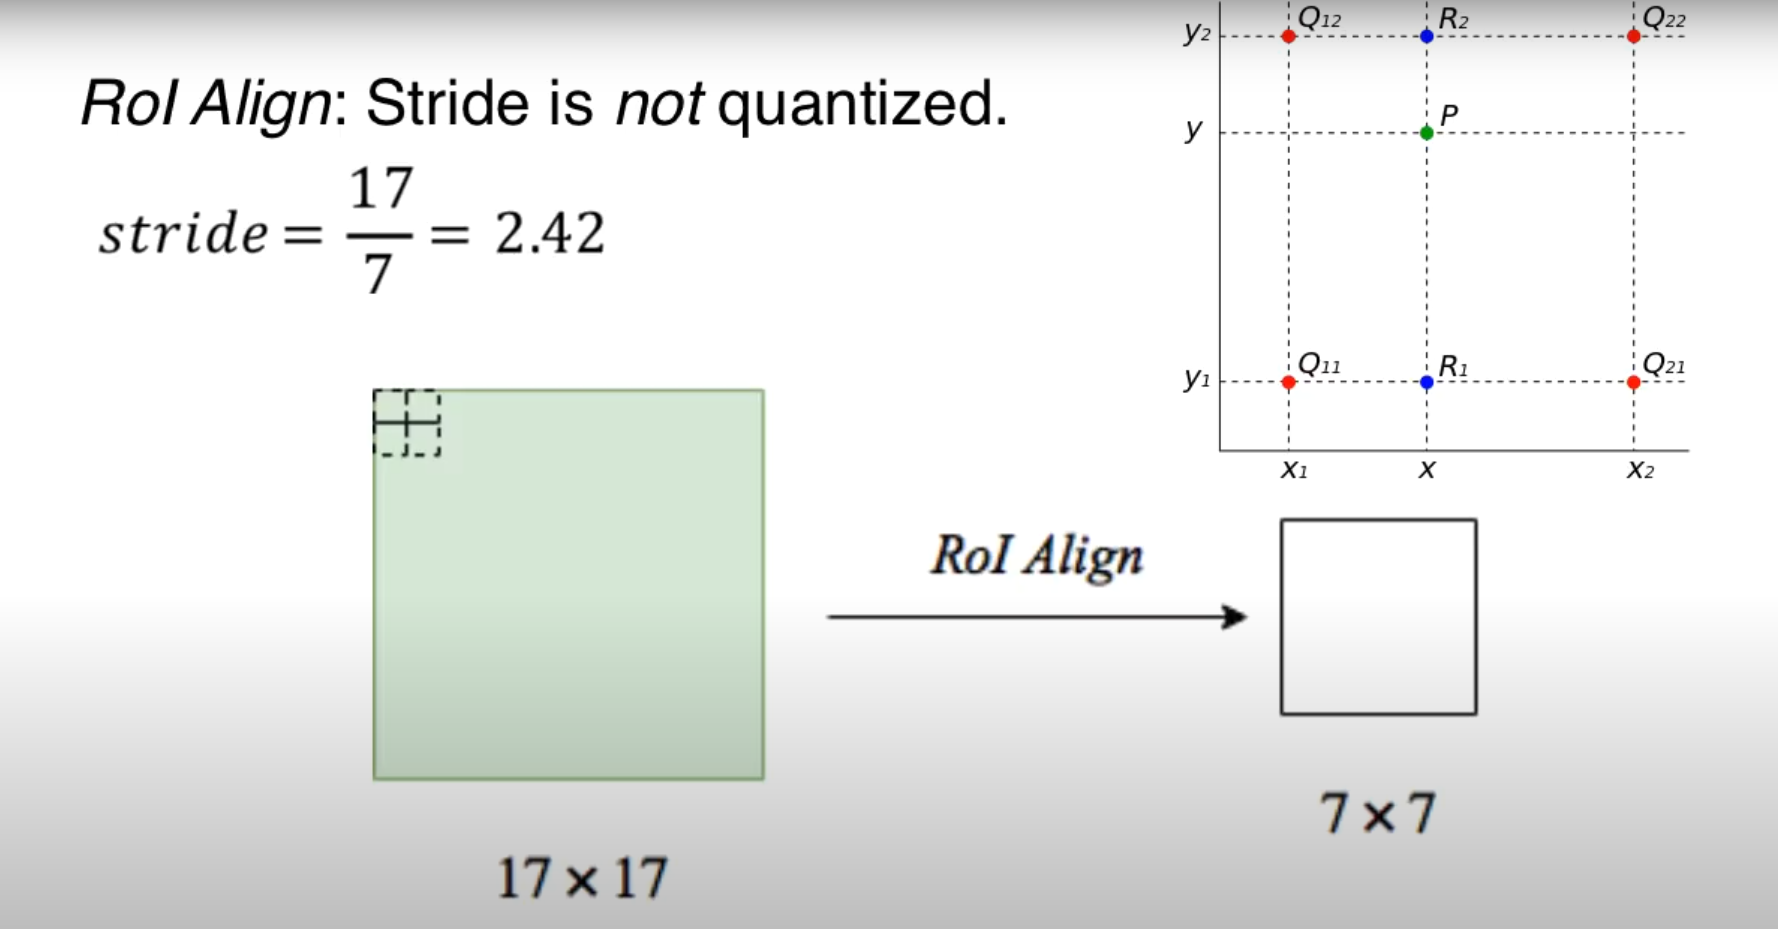
\includegraphics[width=0.85\textwidth]{images/m3_roi_align.png}
    \caption{RoI Align: Unlike RoI Pooling, the stride is NOT quantized (stride $= 17/7 = 2.42$ kept as float). Bilinear interpolation at fractional grid points (using the four nearest neighbours $Q_{11}, Q_{21}, Q_{12}, Q_{22}$) eliminates quantization misalignment, critical for Mask R-CNN pixel-level predictions. (Source: CV Module 3)}
    \label{fig:m3_roi_align}
\end{figure}

\subsection{Mask R-CNN}

\begin{figure}[H]
    \centering
    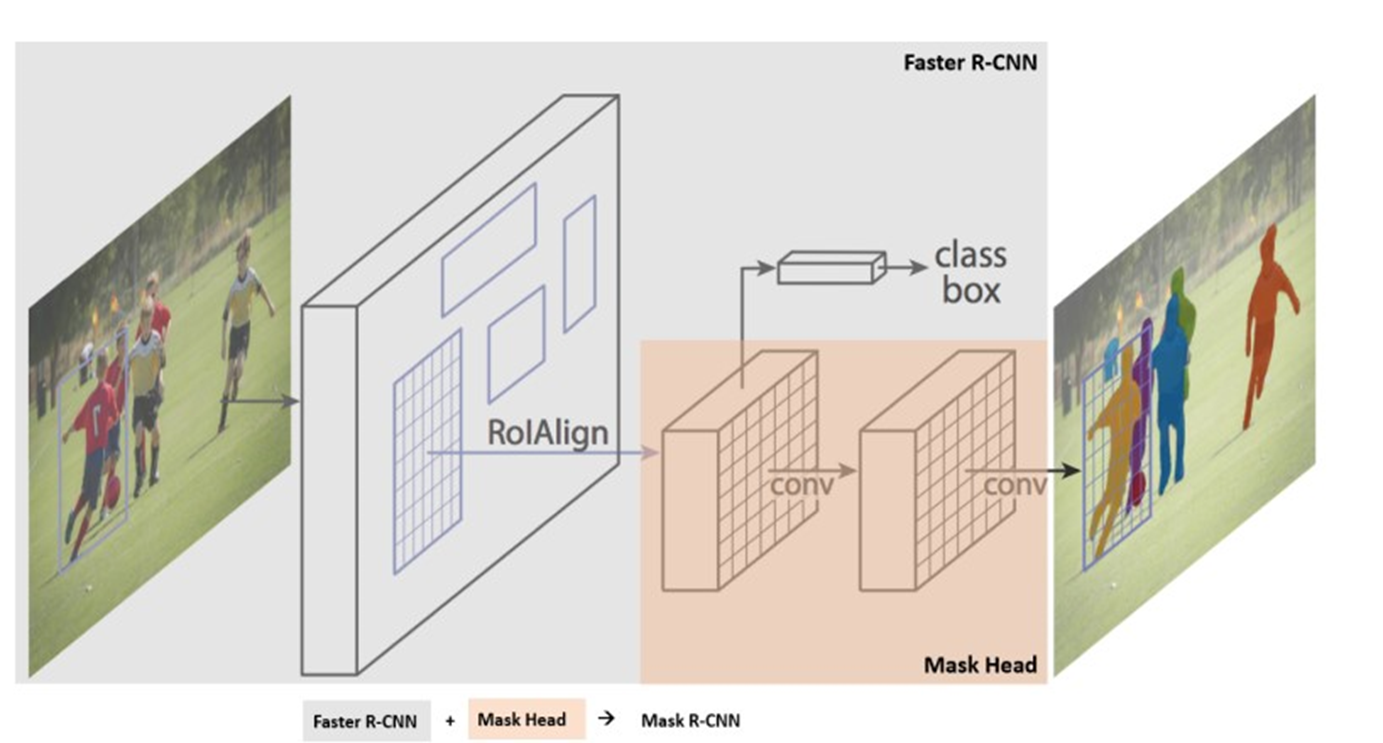
\includegraphics[width=0.85\textwidth]{images/m3_mask_rcnn_arch.png}
    \caption{Mask R-CNN = Faster R-CNN + Mask Head: Feature map $\to$ RoIAlign extracts aligned region features $\to$ two conv layers (Mask Head) predict a per-class binary mask in parallel with the existing class and box heads. Enables instance segmentation (each person gets a unique colour mask). (Source: CV Module 3)}
    \label{fig:m3_mask_rcnn}
\end{figure}

\subsection{Semantic vs.~Instance Segmentation}

\begin{figure}[H]
    \centering
    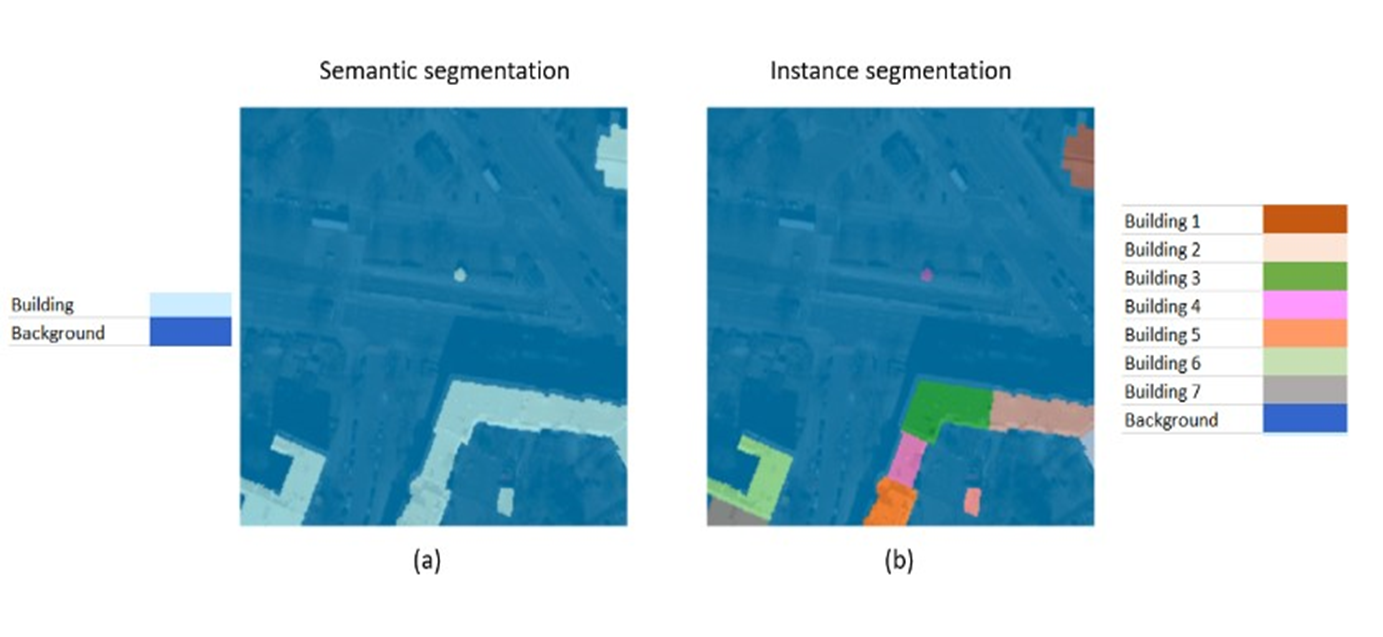
\includegraphics[width=0.85\textwidth]{images/m3_semantic_vs_instance_seg.png}
    \caption{Semantic segmentation (left) labels all pixels of the same class identically (all buildings share one colour). Instance segmentation (right) distinguishes individual instances of the same class (Building 1, Building 2, \ldots{} each get a unique colour). (Source: CV Module 3)}
    \label{fig:m3_sem_vs_inst}
\end{figure}

\subsection{Face Recognition: Siamese Networks}

\begin{figure}[H]
    \centering
    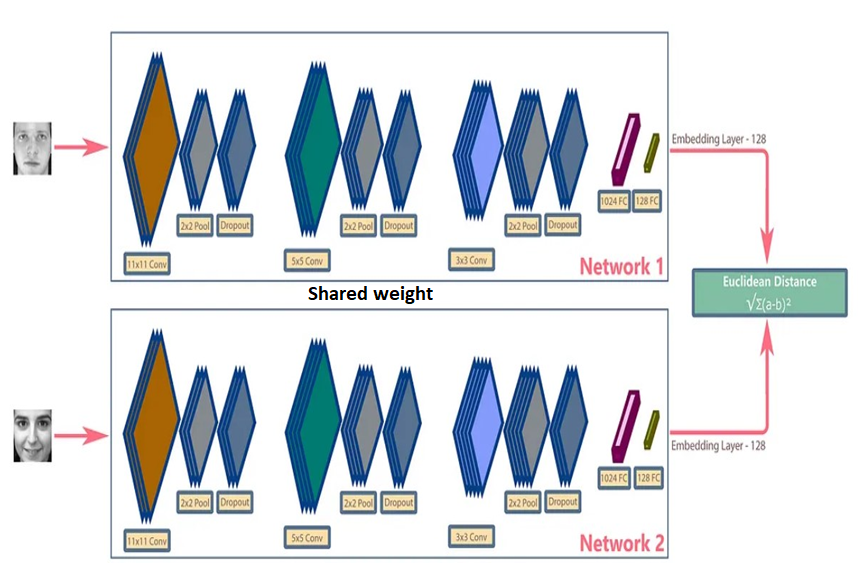
\includegraphics[width=0.85\textwidth]{images/m3_siamese_network.png}
    \caption{Siamese Network Architecture: Two identical CNNs (shared weights) process two input face images independently into 128-d embedding vectors; Euclidean distance $\sqrt{\sum(a-b)^2}$ between embeddings determines similarity. Small distance $\Rightarrow$ same person; large distance $\Rightarrow$ different person. (Source: CV Module 3)}
    \label{fig:m3_siamese}
\end{figure}

\begin{figure}[H]
    \centering
    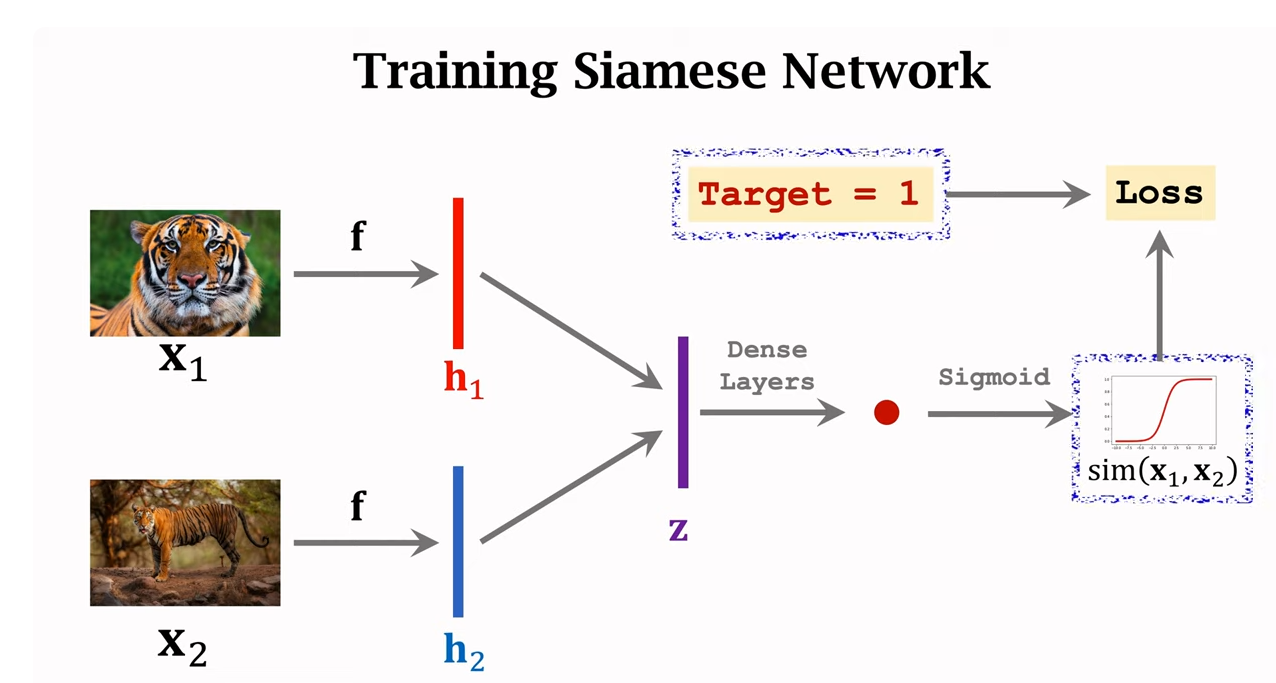
\includegraphics[width=0.85\textwidth]{images/m3_siamese_training.png}
    \caption{Training a Siamese Network: Two images ($x_1$, $x_2$) pass through shared function $f$ to produce embeddings $h_1$, $h_2$; combined via dense layers $\to$ sigmoid similarity score $\text{sim}(x_1,x_2)$; compared with target label (1 = same class) to compute loss via backpropagation. (Source: CV Module 3)}
    \label{fig:m3_siamese_train}
\end{figure}

\subsection{Zero-Shot, One-Shot, and Few-Shot Learning}

\begin{figure}[H]
    \centering
    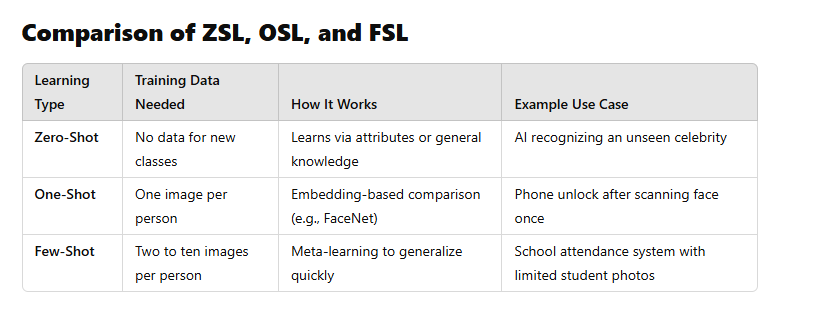
\includegraphics[width=0.85\textwidth]{images/m3_zsl_osl_fsl_table.png}
    \caption{Comparison of Zero-Shot (ZSL), One-Shot (OSL), and Few-Shot (FSL) Learning: ZSL uses attributes or general knowledge with no labelled examples; OSL uses embedding-based comparison (e.g., FaceNet) with one image per class; FSL uses meta-learning with 2--10 images per class. (Source: CV Module 3)}
    \label{fig:m3_zsl}
\end{figure}

\subsection{Loss Functions for Object Detection}

\subsubsection{Contrastive Loss}

Used in Siamese networks to learn embeddings where similar objects are close together and dissimilar objects are far apart:
\[
L = \frac{1}{2} (1 - Y) D^2 + \frac{1}{2} Y \max(0, m - D)^2
\]
where $Y = 1$ if same class, $Y = 0$ if different class, $D$ = distance between embeddings, $m$ = margin.

\subsubsection{Triplet Loss}

Used to learn discriminative features by comparing an anchor, a positive (same class), and a negative (different class):
\[
L = \max(0, D(a, p)^2 - D(a, n)^2 + \alpha)
\]
where $a$ = anchor, $p$ = positive, $n$ = negative, $\alpha$ = margin.

\begin{tcolorbox}[colback=yellow!5!white,colframe=yellow!75!black,title=\textbf{Worked Example 11: Triplet Loss Calculation}]
\textbf{Given}: Anchor embedding $a = [1, 0]$, Positive $p = [0.9, 0.1]$, Negative $n = [0.1, 0.8]$, Margin $\alpha = 0.2$.

\textbf{Step 1}: Compute Euclidean distances:
\[
D(a,p) = \sqrt{(1-0.9)^2 + (0-0.1)^2} = \sqrt{0.01 + 0.01} = \sqrt{0.02} \approx 0.141
\]
\[
D(a,n) = \sqrt{(1-0.1)^2 + (0-0.8)^2} = \sqrt{0.81 + 0.64} = \sqrt{1.45} \approx 1.204
\]

\textbf{Step 2}: Compute triplet loss:
\[
L = \max(0, 0.141^2 - 1.204^2 + 0.2) = \max(0, 0.02 - 1.45 + 0.2) = \max(0, -1.23) = 0
\]

\textbf{Interpretation}: Loss is 0 because the anchor is already much closer to the positive than to the negative. The model does not need to update.
\end{tcolorbox}

\newpage

\section{Module 4: Generative Adversarial Networks (GANs)}

\subsection{Introduction to GANs}

A \textbf{Generative Adversarial Network (GAN)} is a deep learning architecture consisting of two competing neural networks: a \textbf{Generator} and a \textbf{Discriminator}. Invented by Ian Goodfellow in 2014.

\textbf{Analogy}: Like a forger (Generator) creating fake currency and a detective (Discriminator) trying to catch the fakes. Through competition, both improve until the fakes are indistinguishable from reality.

\subsection{Core Architecture and Process}

\begin{figure}[H]
    \centering
    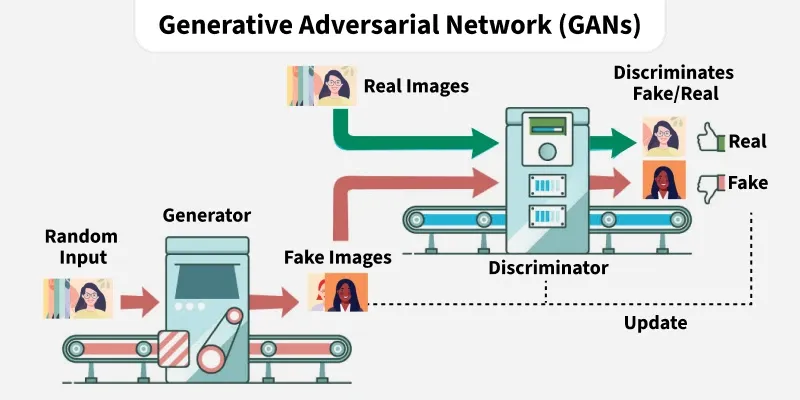
\includegraphics[width=0.85\textwidth]{images/m4_gan_overview.png}
    \caption{Generative Adversarial Network (GAN) Overview: Random input $\to$ Generator produces Fake Images; real images and fake images both enter the Discriminator which outputs Real/Fake; Discriminator loss is backpropagated to update both networks in a minimax game. (Source: CV Module 4)}
    \label{fig:m4_gan_overview}
\end{figure}

\begin{figure}[H]
    \centering
    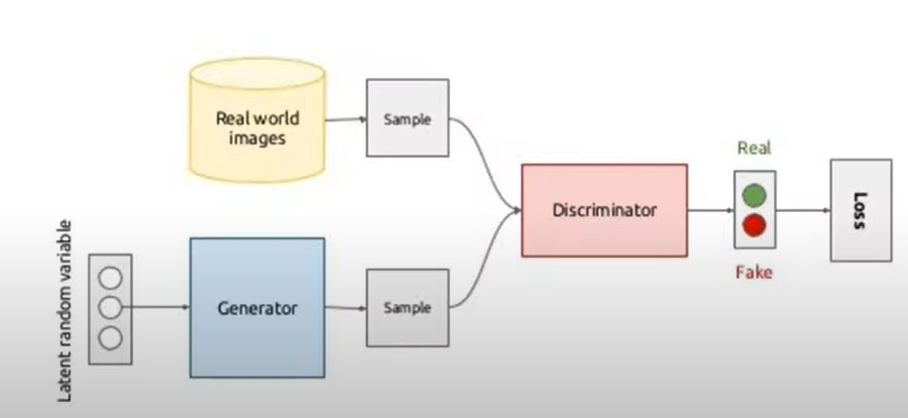
\includegraphics[width=0.85\textwidth]{images/m4_gan_block_diagram.png}
    \caption{GAN Block Diagram: Real-world images database samples real data; latent random variable $z$ fed to Generator which produces fake samples; both paths enter the Discriminator which outputs Real/Fake classification and computes a loss used for backpropagation. (Source: CV Module 4)}
    \label{fig:m4_gan_block}
\end{figure}

\begin{itemize}
    \item \textbf{Generator (G)}:
    \begin{itemize}
        \item \textbf{Input}: Random noise (latent vector).
        \item \textbf{Output}: Fake data (e.g., generated images).
        \item \textbf{Goal}: Produce data so realistic that it fools the Discriminator.
    \end{itemize}
    \item \textbf{Discriminator (D)}:
    \begin{itemize}
        \item \textbf{Input}: Real data (from the training set) and Fake data (from the Generator).
        \item \textbf{Output}: Probability score (0 = Fake, 1 = Real).
        \item \textbf{Goal}: Accurately distinguish between real and fake data.
    \end{itemize}
\end{itemize}

\begin{tcolorbox}[colback=blue!5!white,colframe=blue!75!black,title=\textbf{Training Loop (Min-Max Loss)}]
\begin{enumerate}
    \item \textbf{Noise Sampling}: Generator takes a random noise vector.
    \item \textbf{Data Generation}: Generator creates a fake image.
    \item \textbf{Discrimination}: Discriminator evaluates the fake image against a real image.
    \item \textbf{Adversarial Training}: Feedback (loss) is sent via backpropagation. The Generator updates weights to minimize the discriminator's accuracy, while the Discriminator updates weights to maximize its accuracy.
\end{enumerate}
\end{tcolorbox}

\textbf{Min-Max Objective Function}:
\[
\min_G \max_D V(D, G) = \mathbb{E}_{x \sim p_{\text{data}}} [\ln D(x)] + \mathbb{E}_{z \sim p_z} [\ln(1 - D(G(z)))]
\]

\subsection{The Role of the Noise Vector}

Why use random noise as input to the Generator?
\begin{itemize}
    \item \textbf{Generate Variety (Diversity)}: Without noise, the generator would produce the exact same output every time. Noise acts as a seed for variation.
    \item \textbf{Learn Data Distribution}: The noise maps a simple distribution (like Gaussian) into a complex, high-dimensional real-data distribution.
    \item \textbf{No Bias}: Noise lacks predefined structures, forcing the model to learn pure data patterns.
\end{itemize}

\subsection{Implicit vs. Explicit Density Estimation}

\begin{itemize}
    \item \textbf{Implicit Density (GANs)}: Learns to generate data that \textit{resembles} the real data distribution without ever explicitly calculating the exact probability distribution.
    \item \textbf{Explicit Density (VAEs - Variational Autoencoders)}: Explicitly learns and computes the probability distribution of data using likelihood (like following an exact recipe).
\end{itemize}

\subsection{Limitations of Vanilla GANs}

\begin{enumerate}
    \item \textbf{Mode Collapse}: The Generator finds a single output (or a small set of outputs) that easily fools the Discriminator and stops producing diverse samples. (e.g., generating the exact same face every time).
    \item \textbf{Training Instability}: If the Discriminator gets too strong too quickly, the Generator receives weak gradients and stops learning. If the Generator is too strong, the Discriminator fails.
    \item \textbf{Vanishing Gradients}: Saturation in the Discriminator's sigmoid activation function can halt the Generator's learning. (Solved partially using Leaky ReLU or different loss functions).
    \item \textbf{Difficult Hyperparameter Tuning}: Highly sensitive to learning rates, batch sizes, and architecture.
\end{enumerate}

\subsection{Advanced GAN Variants}

\begin{itemize}
    \item \textbf{CGAN (Conditional GAN)}: Takes an additional \textit{label} as input. The label dictates the \textit{category} (e.g., ``rose''), while the noise vector dictates the \textit{variation} (shape, color).
    \item \textbf{DCGAN (Deep Convolutional GAN)}: Replaces fully connected layers with Convolutional Neural Networks (CNNs). Uses Strided Convolutions (instead of pooling), Batch Normalization, and Leaky ReLU.
    \item \textbf{WGAN (Wasserstein GAN)}: Replaces standard divergence loss with the Wasserstein distance (Earth Mover's Distance) to measure differences between real/fake, drastically improving training stability.
    \item \textbf{ProGAN (Progressive GAN)}: Starts generating low-resolution images and progressively adds layers to increase resolution and detail.
    \item \textbf{StyleGAN}: Allows fine-grained control over the generated image's style (e.g., pose, lighting, texture).
\end{itemize}

\begin{figure}[H]
    \centering
    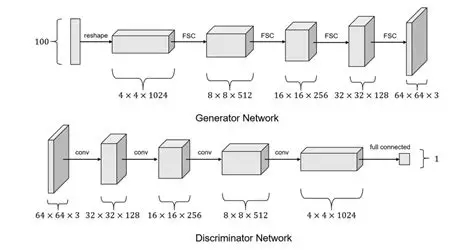
\includegraphics[width=0.85\textwidth]{images/m4_dcgan_arch.png}
    \caption{DCGAN Architecture: Generator (top) --- $100$-d noise $\to$ reshape $\to$ successive FSC (fractionally-strided conv / transposed conv) layers upsampling $4\times4\times1024 \to 64\times64\times3$. Discriminator (bottom) --- mirror of generator using strided convolutions downsampling $64\times64\times3 \to$ single real/fake score. (Source: CV Module 4)}
    \label{fig:m4_dcgan}
\end{figure}

\begin{figure}[H]
    \centering
    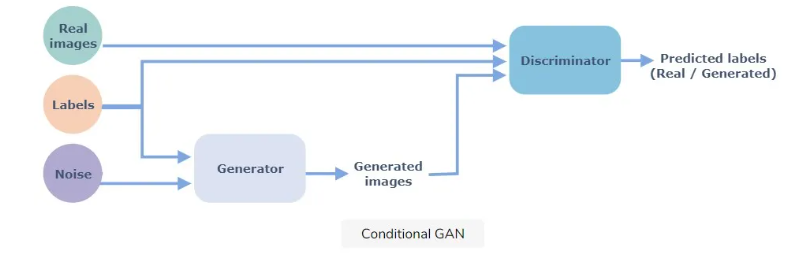
\includegraphics[width=0.85\textwidth]{images/m4_conditional_gan.png}
    \caption{Conditional GAN (CGAN): Real images, class labels, and noise are all fed to the Discriminator; noise + labels are fed to the Generator. The label conditions both networks so the generator produces images of a specific requested class. (Source: CV Module 4)}
    \label{fig:m4_cgan}
\end{figure}

\begin{figure}[H]
    \centering
    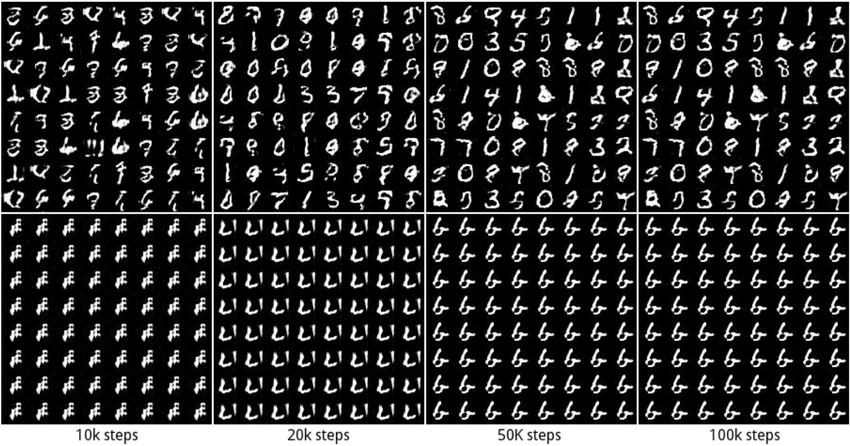
\includegraphics[width=0.85\textwidth]{images/m4_dcgan_training_steps.png}
    \caption{DCGAN Training Progress: Digit grids at 10k, 20k, 50k, and 100k training steps show how the generator improves from noise to recognisable and diverse digit images over training. (Source: CV Module 4)}
    \label{fig:m4_dcgan_train}
\end{figure}

\begin{figure}[H]
    \centering
    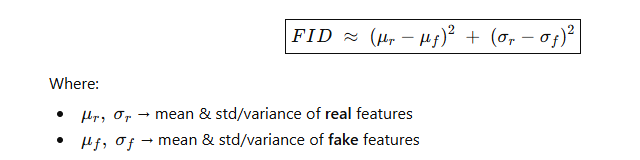
\includegraphics[width=0.85\textwidth]{images/m4_fid_formula.png}
    \caption{Fr\'{e}chet Inception Distance (FID) formula: $\text{FID} \approx (\mu_r - \mu_f)^2 + (\sigma_r - \sigma_f)^2$ where $\mu_r, \sigma_r$ are mean and std of real image features and $\mu_f, \sigma_f$ are mean and std of fake image features from an Inception network. Lower FID = better quality. (Source: CV Module 4)}
    \label{fig:m4_fid}
\end{figure}

\subsection{Solved Numericals: Module 4}

\begin{tcolorbox}[colback=blue!5!white,colframe=blue!75!black,title=\textbf{Worked Example 12: Discriminator Loss Calculation}]
\textbf{Given}:
\begin{itemize}
    \item $D(x) = 0.9$ (Discriminator's probability output for a real image)
    \item $D(G(z)) = 0.3$ (Discriminator's probability output for a fake image)
\end{itemize}

\textbf{Objective}: Calculate the Discriminator's Loss.

\textbf{Steps}:
\begin{enumerate}
    \item \textbf{Formula}: The Discriminator Loss (using natural logarithm) is defined as:
    \[ \text{Loss}_D = - [ \ln(D(x)) + \ln(1 - D(G(z))) ] \]
    \item \textbf{Substitute values}:
    \[ \text{Loss}_D = - [ \ln(0.9) + \ln(1 - 0.3) ] \]
    \[ \text{Loss}_D = - [ \ln(0.9) + \ln(0.7) ] \]
    \item \textbf{Calculate logarithms}:
    \[ \ln(0.9) \approx -0.105, \quad \ln(0.7) \approx -0.357 \]
    \item \textbf{Final calculation}:
    \[ \text{Loss}_D = - ( -0.105 - 0.357 ) = - ( -0.462 ) = 0.462 \]
\end{enumerate}
\textbf{Interpretation}: A lower loss indicates the Discriminator is doing well. 0.462 is relatively low, meaning it correctly identified the real image (0.9 is close to 1) and the fake image (0.3 is close to 0).
\end{tcolorbox}

\vspace{1em}

\begin{tcolorbox}[colback=blue!5!white,colframe=blue!75!black,title=\textbf{Worked Example 13: KL and JS Divergence}]
\textbf{Given}:
\begin{itemize}
    \item Real Distribution $P = [0.5, 0.3, 0.2]$
    \item Predicted Distribution $Q = [0.2, 0.2, 0.6]$
\end{itemize}

\textbf{Objective}: Compute Kullback-Leibler (KL) Divergence and Jensen-Shannon Divergence (JSD).

\textbf{Part 1: KL Divergence ($D_{KL}(P || M)$ and $D_{KL}(Q || M)$)}
\begin{enumerate}
    \item \textbf{Find average distribution $M$}:
    \[ M = \frac{1}{2}(P + Q) = \left[ \frac{0.5+0.2}{2}, \frac{0.3+0.2}{2}, \frac{0.2+0.6}{2} \right] = [0.35, 0.25, 0.4] \]
    \item \textbf{Compute $D_{KL}(P || M)$}:
    \[ D_{KL}(P || M) = \sum P(x) \ln\left(\frac{P(x)}{M(x)}\right) \]
    \begin{itemize}
        \item $0.5 \ln(0.5 / 0.35) = 0.5 \ln(1.428) = 0.178$
        \item $0.3 \ln(0.3 / 0.25) = 0.3 \ln(1.2) = 0.0546$
        \item $0.2 \ln(0.2 / 0.4) = 0.2 \ln(0.5) = -0.1386$
    \end{itemize}
    \[ D_{KL}(P || M) = 0.178 + 0.0546 - 0.1386 = 0.094 \]
    \item \textbf{Compute $D_{KL}(Q || M)$}:
    \[ D_{KL}(Q || M) = \sum Q(x) \ln\left(\frac{Q(x)}{M(x)}\right) \]
    \begin{itemize}
        \item $0.2 \ln(0.2 / 0.35) = -0.112$
        \item $0.2 \ln(0.2 / 0.25) = -0.0446$
        \item $0.6 \ln(0.6 / 0.4) = 0.243$
    \end{itemize}
    \[ D_{KL}(Q || M) = -0.112 - 0.0446 + 0.243 = 0.0864 \]
\end{enumerate}

\textbf{Part 2: Jensen-Shannon Divergence (JSD)}
\begin{enumerate}
    \item \textbf{Formula}:
    \[ \text{JSD}(P || Q) = \frac{1}{2} D_{KL}(P || M) + \frac{1}{2} D_{KL}(Q || M) \]
    \item \textbf{Calculate}:
    \[ \text{JSD}(P || Q) = \frac{1}{2} (0.094 + 0.0864) = \frac{0.1804}{2} = 0.0902 \]
\end{enumerate}
\textbf{Interpretation}: JSD is symmetric and always finite ($0 \le JSD \le 1$ with base 2). Here, JSD $\approx 0.0902$, indicating a low-to-moderate difference between the distributions.
\end{tcolorbox}

\newpage

\section{Module 5: Object Segmentation}

\subsection{Introduction to Segmentation}

\textbf{Image segmentation} is the process of grouping pixels with similar visual characteristics into meaningful segments. It is essentially clustering in the spatial domain.

\textbf{Resolution \& DPI}: $1024 \times 768$ resolution = 786,432 pixels. DPI (Dots Per Inch) determines physical print size/quality, while PPI (Pixels Per Inch) is for screens.

\subsection{Types of Segmentation}

\begin{itemize}
    \item \textbf{Semantic Segmentation}: Classifies every pixel into a category (e.g., all cars get the same ``car'' label). Cannot differentiate between two distinct cars next to each other.
    \item \textbf{Instance Segmentation}: Detects individual object instances. If there are two cars, they are labeled as ``Car 1'' and ``Car 2''.
    \item \textbf{Panoptic Segmentation}: Combines both. Uses the concepts of \textbf{Things} (countable objects with boundaries, like cars and people) and \textbf{Stuff} (uncountable regions without strict boundaries, like sky, grass, road).
\end{itemize}

\textbf{Things vs Stuff in Panoptic Segmentation}:
\begin{itemize}
    \item \textbf{Things}: Countable and distinct object instances with well-defined boundaries (cars, people, animals, furniture).
    \item \textbf{Stuff}: Uncountable regions without well-defined boundaries (sky, road, grass, walls).
\end{itemize}

\subsection{Convolutional Receptive Fields and Pyramids}

\begin{itemize}
    \item \textbf{Receptive Field}: The area of the input image that a neuron ``sees''. Shallow layers see small patches (high resolution, edge details). Deep layers see large regions (low resolution, strong semantic meaning).
    \item \textbf{Image Pyramid}: Manually resizing the image multiple times to detect objects at different scales (computationally expensive).
\end{itemize}

\subsection{Key Segmentation Architectures}

\subsubsection{FPN (Feature Pyramid Network)}

Solves multi-scale detection without multiple image passes.
\begin{itemize}
    \item \textbf{Bottom-Up Pathway}: Normal CNN extracting features (spatial resolution drops, semantic meaning increases).
    \item \textbf{Top-Down Pathway}: Upsamples deep, low-resolution layers.
    \item \textbf{Lateral Connections}: Combines the upsampled deep layers with corresponding shallow layers using 1x1 convolutions. Merges semantic strength with spatial detail.
\end{itemize}

\begin{figure}[H]
    \centering
    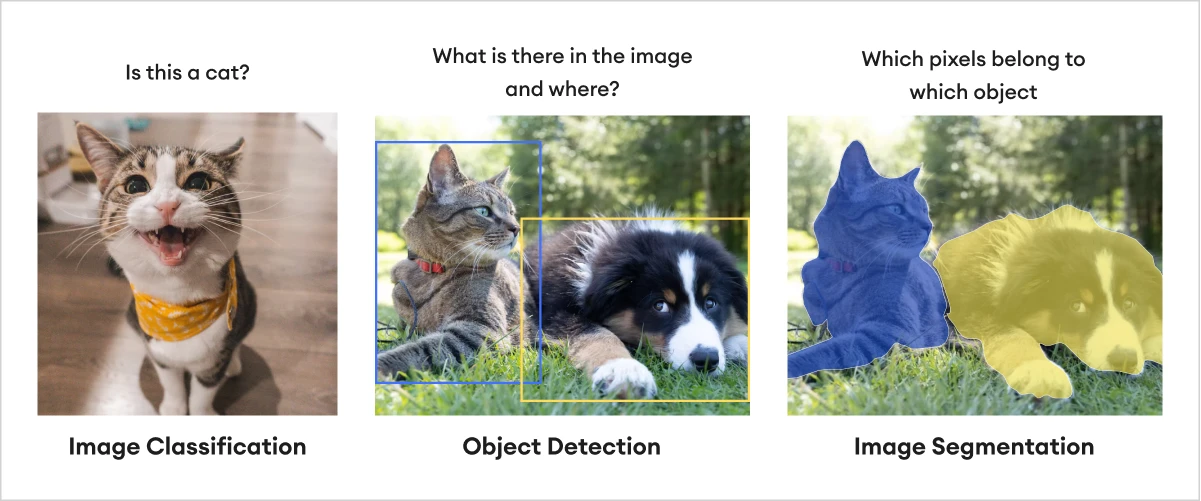
\includegraphics[width=0.85\textwidth]{images/m5_classification_detection_segmentation.png}
    \caption{Image Classification vs.~Object Detection vs.~Image Segmentation: Classification answers ``Is this a cat?''; Detection answers ``What and where?'' with bounding boxes; Segmentation answers ``Which pixels belong to which object?'' with pixel-level masks. (Source: CV Module 5)}
    \label{fig:m5_task_compare}
\end{figure}

\begin{figure}[H]
    \centering
    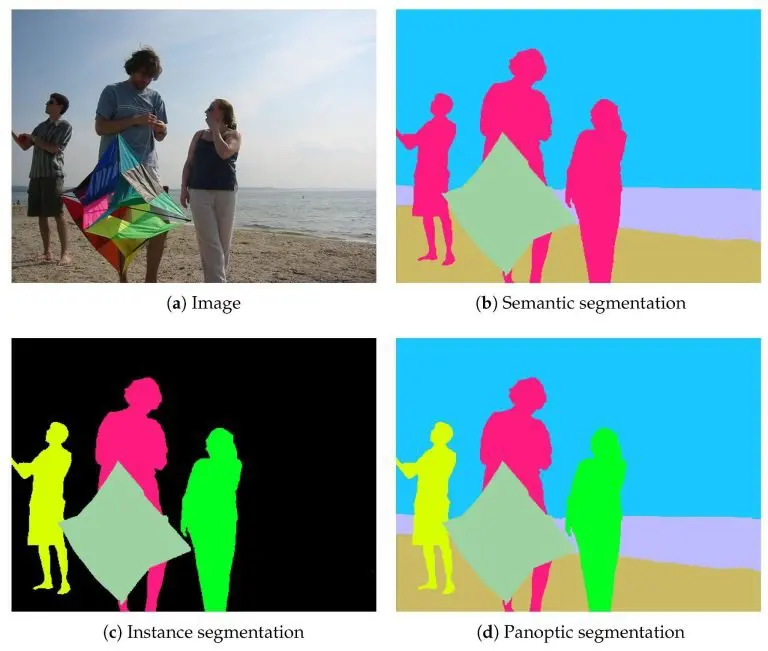
\includegraphics[width=0.85\textwidth]{images/m5_semantic_instance_panoptic.png}
    \caption{Segmentation types: (a) Original image; (b) Semantic segmentation --- all people share one class colour; (c) Instance segmentation --- each person instance gets a unique colour on black background; (d) Panoptic segmentation --- combines semantic background (sky, sand) with instance-aware foreground objects. (Source: CV Module 5)}
    \label{fig:m5_seg_types}
\end{figure}

\begin{figure}[H]
    \centering
    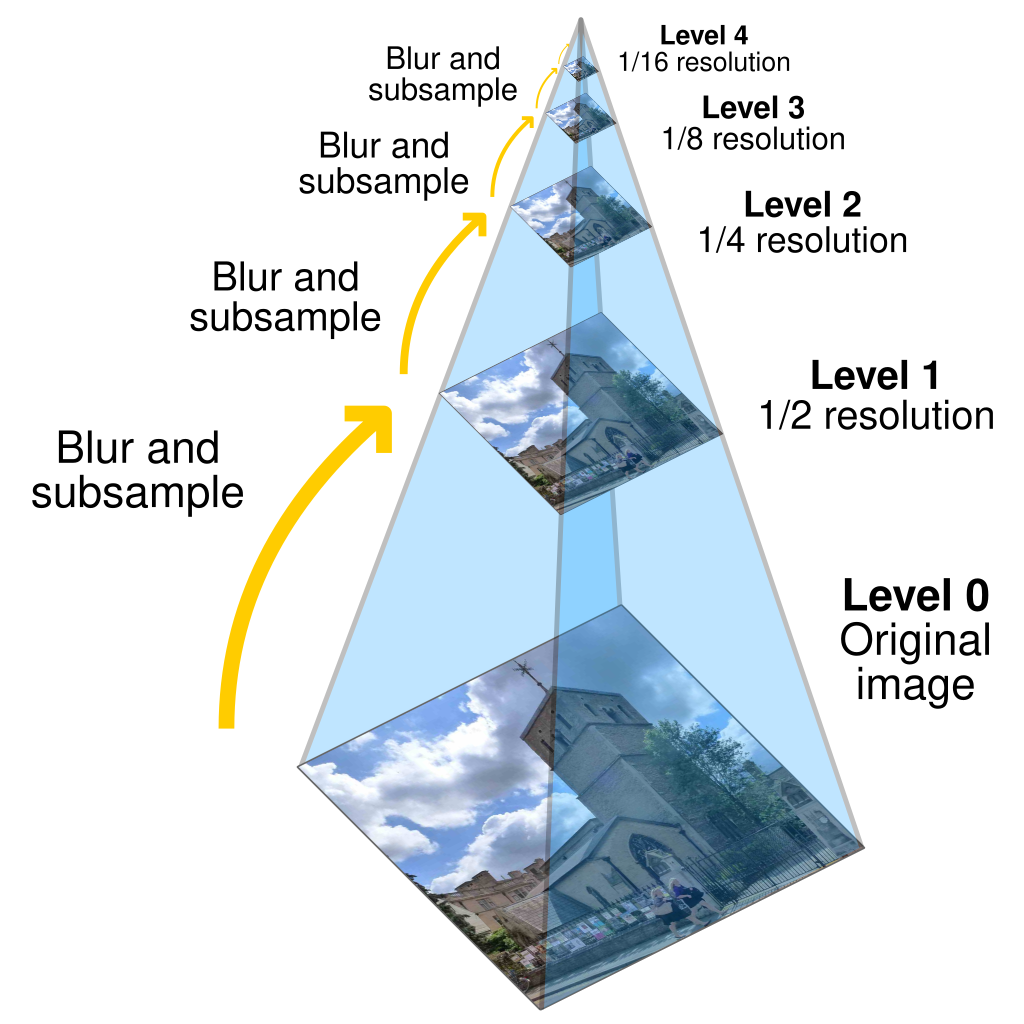
\includegraphics[width=0.5\textwidth]{images/m5_image_pyramid_levels.png}
    \caption{Image Pyramid (Gaussian Pyramid): Original image (Level 0) is progressively blurred and subsampled to produce Levels 1--4 at $1/2$, $1/4$, $1/8$, $1/16$ resolution. Used to detect objects at multiple scales. (Source: CV Module 5)}
    \label{fig:m5_pyramid}
\end{figure}

\begin{figure}[H]
    \centering
    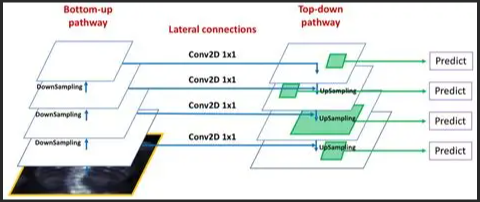
\includegraphics[width=0.85\textwidth]{images/m5_fpn_arch.png}
    \caption{Feature Pyramid Network (FPN) Architecture: Bottom-up pathway (left) --- standard CNN downsampling with increasing semantics; Top-down pathway (right) --- upsampling deep features; Lateral connections --- $1\times1$ Conv2D fuses bottom-up and top-down features at each scale; each level produces a prediction independently. (Source: CV Module 5)}
    \label{fig:m5_fpn}
\end{figure}

\subsubsection{PSPNet (Pyramid Scene Parsing Network)}

Uses a \textbf{Pyramid Pooling Module} that divides the feature map into different grid sizes ($1\times1$, $2\times2$, $3\times3$, $6\times6$) to capture local and global contexts simultaneously. These are upsampled and concatenated before final pixel-wise softmax prediction.

\begin{figure}[H]
    \centering
    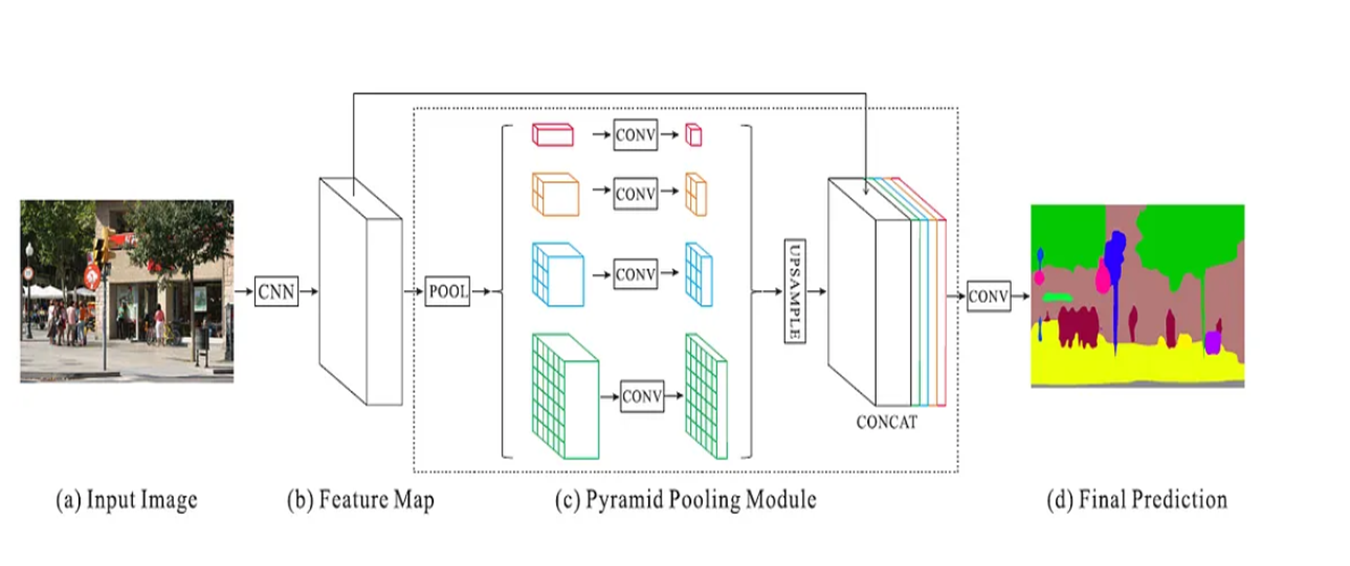
\includegraphics[width=0.85\textwidth]{images/m5_pspnet_arch.png}
    \caption{PSPNet Architecture: (a) Input image $\to$ (b) CNN feature map $\to$ (c) Pyramid Pooling Module applies pooling at $1\times1$, $2\times2$, $3\times3$, $6\times6$ grids, each followed by a $1\times1$ Conv to reduce channels; upsampled outputs are CONCATENATED with the original feature map $\to$ (d) Final $1\times1$ Conv produces pixel-wise segmentation map. (Source: CV Module 5)}
    \label{fig:m5_pspnet}
\end{figure}

\begin{figure}[H]
    \centering
    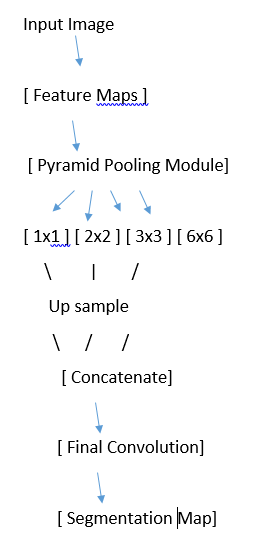
\includegraphics[width=0.6\textwidth]{images/m5_pspnet_pipeline.png}
    \caption{PSPNet Pipeline (simplified): Input Image $\to$ Feature Maps $\to$ Pyramid Pooling Module (1x1, 2x2, 3x3, 6x6 pooling) $\to$ Upsample each $\to$ Concatenate $\to$ Final Convolution $\to$ Segmentation Map. (Source: CV Module 5)}
    \label{fig:m5_pspnet_pipeline}
\end{figure}

\subsubsection{U-Net (Widely used in Medical Imaging)}

\begin{itemize}
    \item \textbf{Contracting Path (Encoder)}: Uses convolutions and pooling to capture context (reduces spatial size).
    \item \textbf{Expansive Path (Decoder)}: Uses transposed convolutions to upsample and restore spatial resolution.
    \item \textbf{Skip Connections}: Crucial feature. Bypasses the deeper layers to directly pass high-resolution spatial details (like edges/boundaries) from the encoder to the decoder, preventing the loss of localization accuracy.
\end{itemize}

\begin{figure}[H]
    \centering
    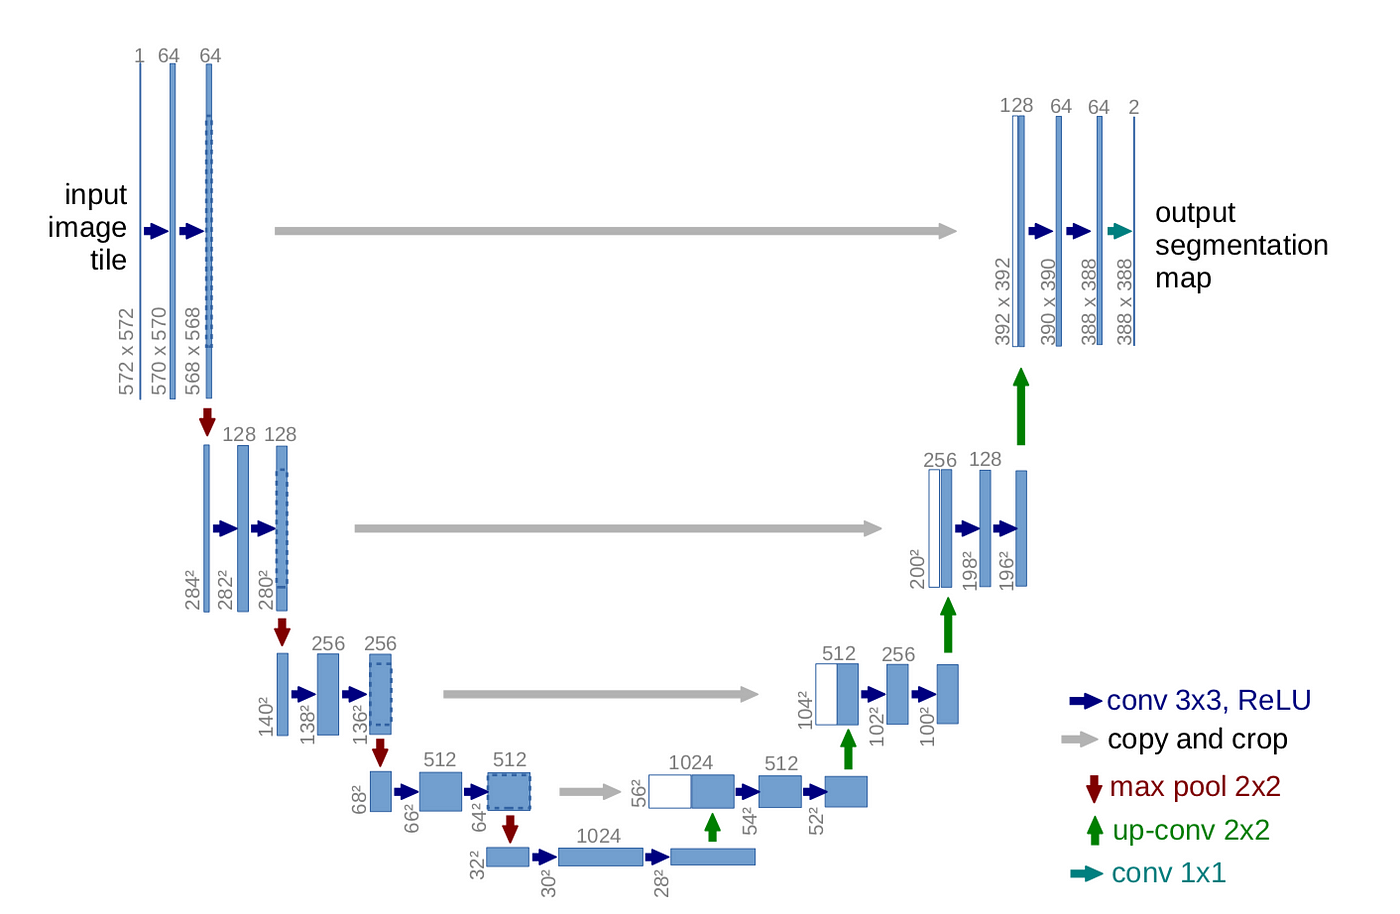
\includegraphics[width=0.85\textwidth]{images/m5_unet_arch.png}
    \caption{U-Net Architecture (original paper): Contracting path (left encoder) uses $3\times3$ conv + ReLU blocks and $2\times2$ max pooling to halve spatial size while doubling channels ($64\to128\to256\to512\to1024$). Expansive path (right decoder) uses $2\times2$ up-conv; skip connections (grey arrows) copy-and-crop encoder feature maps to matching decoder layers. Final $1\times1$ conv outputs the segmentation map. (Source: CV Module 5)}
    \label{fig:m5_unet}
\end{figure}

\begin{figure}[H]
    \centering
    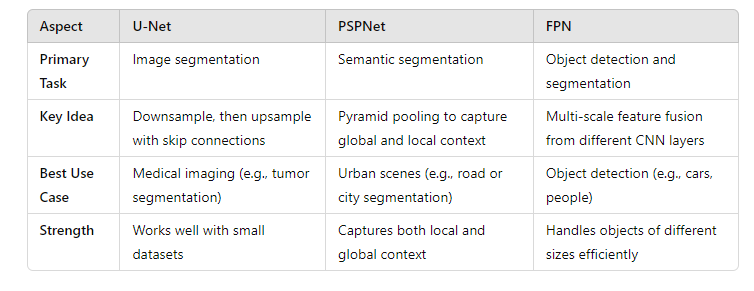
\includegraphics[width=0.85\textwidth]{images/m5_unet_pspnet_fpn_comparison.png}
    \caption{Architecture Comparison --- U-Net vs.~PSPNet vs.~FPN: U-Net excels at medical image segmentation with skip connections; PSPNet uses pyramid pooling for urban scene parsing; FPN uses multi-scale feature fusion for object detection and segmentation. (Source: CV Module 5)}
    \label{fig:m5_arch_compare}
\end{figure}

\subsection{Clustering Methods for Segmentation}

\begin{itemize}
    \item \textbf{K-Means}: Groups pixels into $K$ predefined clusters based on similarity (minimizing variance).
    \item \textbf{Mean Shift}: Does not require predefined $K$. Finds clusters by moving data points towards areas of highest density.
    \item \textbf{DBSCAN}: Density-based. Groups closely packed pixels and isolates outliers/noise. Good for irregular shapes.
    \item \textbf{Agglomerative Hierarchical}: Builds a hierarchy by merging smaller clusters into larger ones. Relies on \textbf{Linkage Criteria}: Single (shortest distance), Complete (longest distance), Average, or Centroid.
\end{itemize}

\subsection{Distance Metrics}

\begin{itemize}
    \item \textbf{Euclidean}: $d = \sqrt{\sum (x_i - y_i)^2}$ --- Straight-line distance (Pythagorean).
    \item \textbf{Manhattan}: $d = \sum |x_i - y_i|$ --- Grid-like distance (sum of absolute differences).
    \item \textbf{Cosine Similarity}: $\cos(\theta) = \frac{A \cdot B}{||A|| \cdot ||B||}$ --- Measures the angle between vectors (ignores magnitude).
    \item \textbf{Minkowski}: Generalized distance formula containing Euclidean and Manhattan.
    \item \textbf{Jaccard Index / Sorensen-Dice}: Measures overlap/similarity between two sets.
\end{itemize}

\subsection{Solved Numericals: Module 5}

\begin{tcolorbox}[colback=gray!5!white,colframe=black!75!black,title=\textbf{Worked Example 14: Bilinear Interpolation (Upsampling)}]
\textbf{Given}:
A low-resolution $2 \times 2$ grid with the following corner pixel values that we wish to upsample into a $4 \times 4$ grid:
\begin{itemize}
    \item Top-left: 10 \quad Top-right: 20
    \item Bottom-left: 30 \quad Bottom-right: 40
\end{itemize}

\textbf{Objective}: Estimate the inner pixel values using bilinear interpolation.

\textbf{Steps}:
\begin{enumerate}
    \item \textbf{Horizontal Interpolation (Rows)}: We have 3 intervals to span between the edges.
    \begin{itemize}
        \item Top Row (10 to 20): Step size = $(20 - 10) / 3 = 3.33$.
        \item Values: $10 \rightarrow 13.3 \rightarrow 16.7 \rightarrow 20$.
        \item Bottom Row (30 to 40): Step size = $(40 - 30) / 3 = 3.33$.
        \item Values: $30 \rightarrow 33.3 \rightarrow 36.7 \rightarrow 40$.
    \end{itemize}

    \item \textbf{Vertical Interpolation (Columns)}: Now interpolate the middle columns vertically. The step size is $(Bottom - Top) / 3$.
    \begin{itemize}
        \item Column 2 (13.3 to 33.3): Step size = $(33.3 - 13.3) / 3 = 6.67$.
        \item Values: $13.3 \rightarrow 20.0 \rightarrow 26.7 \rightarrow 33.3$.
        \item Column 3 (16.7 to 36.7): Step size = $(36.7 - 16.7) / 3 = 6.67$.
        \item Values: $16.7 \rightarrow 23.3 \rightarrow 30.0 \rightarrow 36.7$.
    \end{itemize}
\end{enumerate}

\textbf{Interpretation}:
The resulting $4 \times 4$ interpolated image matrix is smoothly transitioned:
\begin{center}
\begin{tabular}{|c|c|c|c|}
\hline
10.0 & 13.3 & 16.7 & 20.0 \\ \hline
16.7 & 20.0 & 23.3 & 26.7 \\ \hline
23.3 & 26.7 & 30.0 & 33.3 \\ \hline
30.0 & 33.3 & 36.7 & 40.0 \\ \hline
\end{tabular}
\end{center}
\end{tcolorbox}

\vspace{1em}

\begin{tcolorbox}[colback=gray!5!white,colframe=black!75!black,title=\textbf{Worked Example 15: IoU and Dice Coefficient}]
\textbf{Given}:
In an image segmentation task, we have the Ground Truth mask ($A$) and the Model's Predicted mask ($B$):
\begin{itemize}
    \item Ground Truth area ($|A|$) = 50 pixels
    \item Predicted area ($|B|$) = 60 pixels
    \item Intersection (correctly predicted pixels, $|A \cap B|$) = 40 pixels
\end{itemize}

\textbf{Objective}: Calculate the Intersection over Union (IoU) and the Dice Coefficient.

\textbf{Steps}:
\begin{enumerate}
    \item \textbf{Intersection over Union (IoU)}:
    \[ \text{Union } |A \cup B| = |A| + |B| - |A \cap B| \]
    \[ |A \cup B| = 50 + 60 - 40 = 70 \text{ pixels} \]
    \[ \text{IoU} = \frac{|A \cap B|}{|A \cup B|} = \frac{40}{70} \approx 0.571 \text{ (or 57.1\%)} \]

    \item \textbf{Dice Coefficient (F1 Score)}:
    \[ \text{Dice} = \frac{2 |A \cap B|}{|A| + |B|} \]
    \[ \text{Dice} = \frac{2 \times 40}{50 + 60} = \frac{80}{110} \approx 0.727 \text{ (or 72.7\%)} \]
\end{enumerate}

\textbf{Interpretation}: Both metrics evaluate segmentation accuracy. IoU penalizes false positives and false negatives more heavily than Dice, which is why IoU (0.57) is lower than Dice (0.72).
\end{tcolorbox}

\newpage

\section{Module 6: Action Recognition and Object Tracking}

\subsection{Video Understanding Basics}

\begin{itemize}
    \item \textbf{Video vs. Image}: An image has only spatial information (width, height). A video adds a \textbf{temporal} dimension ($x, y, t$).
    \item \textbf{Why Temporal Matters}: A single frame of a person with hands together could be praying, clapping, or resting. A sequence of frames defines the action.
    \item \textbf{Action Recognition}: ``What is happening?'' (e.g., running, fighting).
    \item \textbf{Object Tracking}: ``Where is it happening over time?'' (Locating an object continuously across frames).
\end{itemize}

\textbf{Real-world pipeline}: Detection $\to$ Tracking $\to$ Action Recognition $\to$ Decision.

\subsection{Motion Capture and Modeling}

\begin{itemize}
    \item \textbf{Marker-based}: Uses reflective markers on joints and infrared cameras. Highly accurate, used in biomechanics and animation.
    \item \textbf{Markerless}: Uses AI/Pose-estimation (e.g., OpenPose, MoveNet) to detect joints from standard video. Non-invasive.
    \item \textbf{Kinematic Models (How things move, ignoring force)}:
    \begin{enumerate}
        \item \textbf{Point Mass Model}: Treats object as a single point. Ignores shape, size, and rotation.
        \item \textbf{Rigid Body Model}: Accounts for shape and rotation, assuming the object doesn't deform.
        \item \textbf{Articulated Body Model}: Multiple rigid bodies connected by joints (e.g., a human body or robotic arm).
    \end{enumerate}
    \item \textbf{Dynamic Models}: Examines \textit{why} things move, analyzing mass, forces, and torques.
\end{itemize}

\subsection{Optical Flow}

\begin{figure}[H]
    \centering
    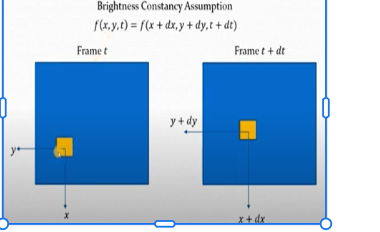
\includegraphics[width=0.7\textwidth]{images/m6_brightness_constancy.png}
    \caption{Brightness Constancy Assumption: A pixel at $(x,y)$ in frame $t$ moves to $(x+dx, y+dy)$ in frame $t+dt$ but its intensity remains constant: $f(x,y,t) = f(x+dx,y+dy,t+dt)$. This constraint underlies all optical flow methods. (Source: CV Module 6)}
    \label{fig:m6_bright_const}
\end{figure}

\textbf{Definition}: The pattern of apparent motion of image objects between two consecutive frames caused by the movement of object or camera.

\textbf{Brightness Constancy Assumption}: The intensity (color/brightness) of a pixel representing a moving object remains constant between frames; only its position ($x,y$) changes.
\[
I_x u + I_y v + I_t = 0
\]
where $I_x, I_y$ are spatial gradients, $I_t$ is temporal gradient, and $(u,v)$ is the optical flow vector.

\textbf{The Aperture Problem}: Viewing motion through a small region makes it impossible to determine the true direction of motion along an edge. Therefore, a single pixel is not enough to calculate optical flow (we have 1 equation but 2 unknowns: $u$ and $v$).

\textbf{Solutions}:
\begin{itemize}
    \item \textbf{Lucas-Kanade Method}: Assumes \textit{Local Motion Consistency} (nearby pixels in a small window move in the same way). Produces \textbf{Sparse Optical Flow} (only tracks key feature points/corners).
    \item \textbf{Horn-Schunck Method}: Assumes \textit{Global Smoothness} (motion changes smoothly across the entire image). Produces \textbf{Dense Optical Flow} (calculates motion vectors for every single pixel).
\end{itemize}

\begin{figure}[H]
    \centering
    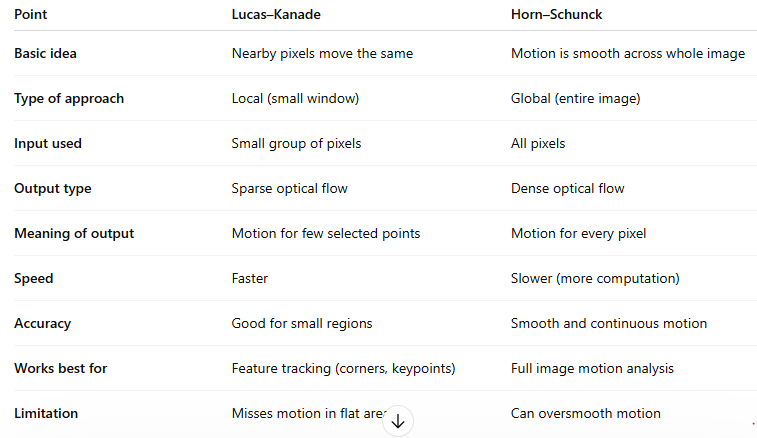
\includegraphics[width=0.85\textwidth]{images/m6_lk_vs_hs_table.png}
    \caption{Lucas-Kanade vs.~Horn-Schunck Comparison: LK is local (small window), produces sparse flow, faster, good for corners; HS is global (entire image), produces dense flow, slower, smooth and continuous. (Source: CV Module 6)}
    \label{fig:m6_lk_vs_hs}
\end{figure}

\subsection{Tracking Methods}

\begin{itemize}
    \item \textbf{Kalman Filter}: A predictive model that estimates an object's future position based on its past trajectory and updates the prediction using new measurements. Fast and efficient for linear motion.
    \begin{itemize}
        \item \textbf{Prediction}: Estimate next state based on current state and motion model.
        \item \textbf{Update}: Correct prediction using actual measurement.
        \item Works best when motion is predictable (linear/Gaussian).
    \end{itemize}
    \item \textbf{Particle Filter}: Used for complex, non-linear motion tracking. Represents the state distribution with a set of weighted particles.
\end{itemize}

\begin{tcolorbox}[colback=green!5!white,colframe=green!50!black,title=\textbf{Case Study: CCTV Surveillance System}]
\textbf{Scenario}: A camera monitors a shopping mall to ensure safety and security.

\textbf{Q1: How will the system follow a person across frames?}
\begin{itemize}
    \item \textbf{Detect}: Identify the person in the initial frame using object detection.
    \item \textbf{Track}: Estimate the person's position in subsequent frames based on appearance and motion models.
    \item \textbf{Update}: Continuously update the person's location vector as they move.
\end{itemize}

\textbf{Q2: How will the system detect suspicious behavior (e.g., fighting)?}
\begin{itemize}
    \item \textbf{Analyze}: Monitor the sequence of spatio-temporal movements across consecutive frames.
    \item \textbf{Identify}: Detect unusual or abnormal motion patterns that deviate from normal walking behavior.
    \item \textbf{Classify}: Use an action recognition classifier to tag the abnormal movement sequence as ``fighting''.
\end{itemize}
\end{tcolorbox}

\subsection{3D Vision and Depth Estimation}

\begin{itemize}
    \item \textbf{Stereo Vision}: Uses two cameras (Left and Right) to estimate depth, mimicking human eyes.
    \item \textbf{Stereo Matching}: Finding the exact same physical point in both the left and right images.
    \item \textbf{Disparity}: The difference in the pixel coordinates of the same point in the two images.
    \item \textbf{Depth Calculation}: Depth is \textbf{inversely proportional} to disparity.
    \begin{itemize}
        \item \textit{Large disparity = Object is close.}
        \item \textit{Small disparity = Object is far away.}
    \end{itemize}
\end{itemize}

\begin{center}
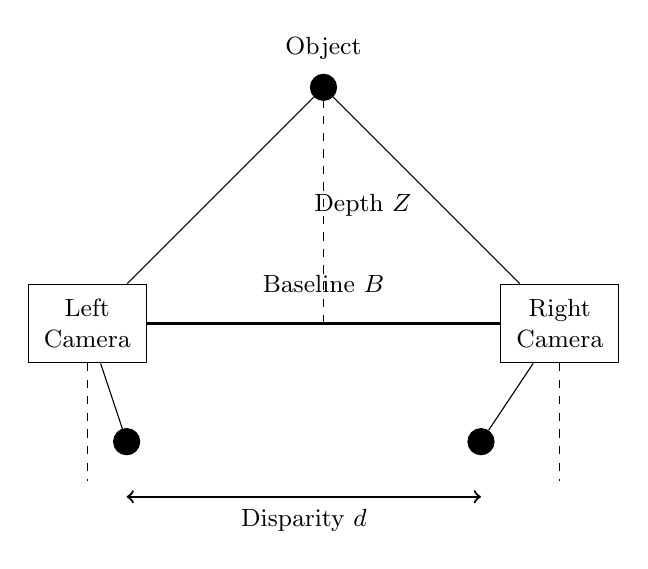
\begin{tikzpicture}[
    node distance=1.5cm,
    cam/.style={rectangle, draw, minimum width=1.5cm, minimum height=1cm, font=\small, align=center},
    point/.style={circle, draw, fill=black, minimum size=0.1cm},
    arrow/.style={->, >=stealth, thick}
]
% Cameras
\node[cam] (left) at (0,0) {Left\\Camera};
\node[cam] (right) at (6,0) {Right\\Camera};

% Baseline
\draw[thick] (left) -- (right);
\node[font=\small] at (3, 0.5) {Baseline $B$};

% Object
\node[point] (obj) at (3, 3) {};
\node[font=\small] at (3, 3.5) {Object};

% Lines of sight
\draw (left) -- (obj);
\draw (right) -- (obj);

% Image planes
\draw[dashed] (0, -0.5) -- (0, -2);
\draw[dashed] (6, -0.5) -- (6, -2);

% Image points
\node[point] (il) at (0.5, -1.5) {};
\node[point] (ir) at (5, -1.5) {};

\draw (left) -- (il);
\draw (right) -- (ir);

% Disparity
\draw[<->, thick] (0.5, -2.2) -- (5, -2.2);
\node[font=\small] at (2.75, -2.5) {Disparity $d$};

% Depth label
\draw[dashed] (3, 0) -- (3, 3);
\node[font=\small] at (3.5, 1.5) {Depth $Z$};

\end{tikzpicture}
\end{center}
\captionof{figure}{Stereo Vision Triangulation: Two cameras separated by baseline $B$ observe the same object. Disparity $d = x_L - x_R$ is inversely proportional to depth $Z$.}

\subsection{Solved Numericals: Module 6}

\begin{tcolorbox}[colback=orange!5!white,colframe=orange!75!black,title=\textbf{Worked Example 16: Optical Flow (Brightness Constancy)}]
\textbf{Given}:
A tracking system observes a pixel moving between two consecutive frames. The image gradients at the pixel are calculated as follows:
\begin{itemize}
    \item Spatial gradient in X-direction ($I_x$) = 2
    \item Spatial gradient in Y-direction ($I_y$) = 3
    \item Temporal gradient ($I_t$) = -12
\end{itemize}
It is known that the object is moving \textbf{purely horizontally} (meaning the vertical velocity component $v = 0$).

\textbf{Objective}: Find the horizontal velocity $u$ of the pixel.

\textbf{Steps}:
\begin{enumerate}
    \item \textbf{Formula}: State the Brightness Constancy Equation:
    \[ I_x u + I_y v + I_t = 0 \]
    \item \textbf{Substitute values}:
    \[ (2)u + (3)(0) + (-12) = 0 \]
    \item \textbf{Solve for $u$}:
    \[ 2u - 12 = 0 \implies 2u = 12 \implies u = 6 \]
\end{enumerate}

\textbf{Interpretation}: The optical flow vector is $(u,v) = (6, 0)$. This means the pixel moved 6 pixels to the right between the two frames.
\end{tcolorbox}

\vspace{1em}

\begin{tcolorbox}[colback=orange!5!white,colframe=orange!75!black,title=\textbf{Worked Example 17: Depth Estimation using Stereo Vision}]
\textbf{Given}:
A stereo vision system has two parallel cameras:
\begin{itemize}
    \item Focal length ($f$) = 50 mm
    \item Baseline distance between cameras ($B$) = 120 mm
    \item An object is detected at $x_L = 400$ in the left image and $x_R = 390$ in the right image (in pixels).
    \item Sensor pixel size = $0.01$ mm/pixel
\end{itemize}

\textbf{Objective}: Calculate the depth ($Z$) of the object from the cameras.

\textbf{Steps}:
\begin{enumerate}
    \item \textbf{Calculate Disparity in pixels}:
    \[ d_{\text{pixels}} = x_L - x_R = 400 - 390 = 10 \text{ pixels} \]
    \item \textbf{Convert Disparity to Physical Units (mm)}:
    \[ d = d_{\text{pixels}} \times \text{pixel size} = 10 \times 0.01 = 0.1 \text{ mm} \]
    \item \textbf{Calculate Depth using Triangulation Formula}:
    \[ Z = \frac{f \cdot B}{d} \]
    \[ Z = \frac{50 \text{ mm} \times 120 \text{ mm}}{0.1 \text{ mm}} \]
    \[ Z = \frac{6000}{0.1} = 60{,}000 \text{ mm} \]
    \item \textbf{Convert to standard units}:
    \[ 60{,}000 \text{ mm} = 60 \text{ meters} \]
\end{enumerate}

\textbf{Interpretation}: The object is 60 meters away from the stereo camera setup. This demonstrates the inverse relationship: a small disparity ($0.1$ mm) corresponds to a large depth ($60$ m).
\end{tcolorbox}

\newpage

\section*{Appendix: Quick Reference Tables}

\subsection*{Numerical Inventory}
\begin{center}
\begin{tabular}{|c|l|c|}
\hline
\textbf{Module} & \textbf{Worked Example} & \textbf{Concept} \\
\hline
1 & WE 1 & Image Memory Calculation \\
1 & WE 2 & Sampling and Quantization \\
1 & WE 3 & DCT Coefficient Energy Compaction \\
1 & WE 4 & Morphological Opening and Closing \\
2 & WE 5 & Chain Code Extraction \\
2 & WE 6 & Iterative Global Thresholding \\
2 & WE 7 & Otsu's Method \\
2 & WE 8 & Hough Transform Line Detection \\
3 & WE 9 & Two-Stage vs One-Stage Comparison \\
3 & WE 10 & IoU, Precision, Recall, and mAP \\
3 & WE 11 & Triplet Loss Calculation \\
4 & WE 12 & Discriminator Loss Calculation \\
4 & WE 13 & KL and JS Divergence \\
5 & WE 14 & Bilinear Interpolation \\
5 & WE 15 & IoU and Dice Coefficient \\
6 & WE 16 & Optical Flow (Brightness Constancy) \\
6 & WE 17 & Depth Estimation (Stereo Vision) \\
\hline
\end{tabular}
\end{center}

\subsection*{TikZ Diagram Inventory}
\begin{center}
\begin{tabular}{|c|l|}
\hline
\textbf{Module} & \textbf{Diagram} \\
\hline
1 & Image Acquisition Pipeline \\
1 & Morphological Operations Concept \\
2 & 8-Directional Freeman Chain Code \\
3 & R-CNN Evolution (R-CNN / Fast R-CNN / Faster R-CNN) \\
3 & YOLO Grid-Based Detection \\
4 & GAN Architecture (Generator + Discriminator) \\
4 & DCGAN Generator Architecture \\
5 & FPN Architecture (Bottom-Up + Top-Down + Lateral) \\
5 & U-Net Encoder-Decoder with Skip Connections \\
6 & Stereo Vision Triangulation \\
\hline
\end{tabular}
\end{center}

\end{document}
